%%%%%%%%%%%%%%%%%%%%%%%%%%%%%%%%%%%%%%%%%%%%%%%%%%%%%%%%%%%%%
%%  Document Type											%
%%%%%%%%%%%%%%%%%%%%%%%%%%%%%%%%%%%%%%%%%%%%%%%%%%%%%%%%%%%%%

% \documentclass[cleanfoot,12pt]{asme2ej}
\documentclass[review]{elsarticle}

%% Set margins 	--------------------------------------------
\usepackage{geometry}
\geometry{letterpaper, portrait, lmargin = 1.0in, rmargin = 1.0in, tmargin=1.0in, bmargin = 1.0in}

%%%%%%%%%%%%%%%%%%%%%%%%%%%%%%%%%%%%%%%%%%%%%%%%%%%%%%%%%%%%%
%%  Package Used											%
%%%%%%%%%%%%%%%%%%%%%%%%%%%%%%%%%%%%%%%%%%%%%%%%%%%%%%%%%%%%%

%-----------------------------------------------------------
%	Topography
%-----------------------------------------------------------
\usepackage{microtype}

\usepackage{setspace} %allow double spacing text
%-----------------------------------------------------------


%-----------------------------------------------------------
%	Important equation editing packages
%-----------------------------------------------------------
\usepackage{amssymb,amsmath,mathtools,commath}
\DeclareMathAlphabet\mathbfcal{OMS}{cmsy}{b}{n}	% Bolded caligraphy font
\usepackage{subdepth} 	% Fix the alignment of subscripts in equations
\allowdisplaybreaks
%-----------------------------------------------------------

%-----------------------------------------------------------
%	For making tables
%-----------------------------------------------------------
\usepackage[table]{xcolor}
\definecolor{Gray}{gray}{0.9}
%-----------------------------------------------------------

%-----------------------------------------------------------
%	For formating citations and hyperlinking
%-----------------------------------------------------------
\usepackage[breaklinks=true]{hyperref}
\usepackage{breakcites}
\usepackage{lineno}
% \modulolinenumbers[5]
%-----------------------------------------------------------

%-----------------------------------------------------------
%	Editing sections and appendix
%-----------------------------------------------------------
\usepackage[titletoc,title]{appendix} 	% Allows the use of appendices
\usepackage[section]{placeins}			% Force figures to be within 
										%	the sections
%-----------------------------------------------------------



%%%%%%%%%%%%%%%%%%%%%%%%%%%%%%%%%%%%%%%%%%%%%%%%%%%%%%%%%%%%%
%%  Nomenclature ASME template does not create nomenclatures%
%%. specified in the Journal format							% 
%%%%%%%%%%%%%%%%%%%%%%%%%%%%%%%%%%%%%%%%%%%%%%%%%%%%%%%%%%%%%

\usepackage{nomencl}
\makenomenclature
\renewcommand{\nomname}{Nomenclature}
%-----------------------------------------------------------
%	Nomenclature
%-----------------------------------------------------------
%% This code creates the groups
%-----------------------------------------------------------
\usepackage{etoolbox}
\renewcommand\nomgroup[1]{%
  \item[\bfseries
  \ifstrequal{#1}{K}{Key Terms}{%
  \ifstrequal{#1}{S}{Symbols}}%
]}
\apptocmd{\thebibliography}{\raggedright}{}{}
%-----------------------------------------------------------
%% This code creates quotes
%-----------------------------------------------------------
\AtBeginEnvironment{quote}{\singlespacing\small}
%-----------------------------------------------------------


%%%%%%%%%%%%%%%%%%%%%%%%%%%%%%%%%%%%%%%%%%%%%%%%%%%%%%%%%%%%%
%%  Making the custom header for specifying the Journal	in	%
%%. accordance to the ASME Journal format specified			%
%%%%%%%%%%%%%%%%%%%%%%%%%%%%%%%%%%%%%%%%%%%%%%%%%%%%%%%%%%%%%
\usepackage{fancyhdr}
%-----------------------------------------------------------
%	The settings are below
%-----------------------------------------------------------
\renewcommand{\headrulewidth}{0pt}	% No horizontal line as 
%	specified
\setlength{\headheight}{13.6pt}		% Adjustment for header 
%	size
\pagestyle{fancy}
\fancyhf{}
\cfoot{\thepage}

%%%%%%%%%%%%%%%%%%%%%%%%%%%%%%%%%%%%%%%%%%%%%%%%%%%%%%%%%%%%%
%%  Pagination as required by the Journal but not included	%
%%. in the Document Class									%
%%%%%%%%%%%%%%%%%%%%%%%%%%%%%%%%%%%%%%%%%%%%%%%%%%%%%%%%%%%%%

% \pagenumbering{arabic}

%%%%%%%%%%%%%%%%%%%%%%%%%%%%%%%%%%%%%%%%%%%%%%%%%%%%%%%%%%%%%
%%  User defined hyphenation								%
%%%%%%%%%%%%%%%%%%%%%%%%%%%%%%%%%%%%%%%%%%%%%%%%%%%%%%%%%%%%%

% \hyphenation{cross-link-ed}

    
    


%%%%%%%%%%%%%%%%%%%%%%%%%%%%%%%%%%%%%%%%%%%%%%%%%%%%%%%%%%%%%
%%	Begin Document											%
%%%%%%%%%%%%%%%%%%%%%%%%%%%%%%%%%%%%%%%%%%%%%%%%%%%%%%%%%%%%%

\begin{document}





% %%%%%%%%%%%%%%%%%%%%%%%%%%%%%%%%%%%%%%%%%%%%%%%%%%%%%%%%%%%%%
% %%  About the Journal and Authors for ASME Journal			%
% %%%%%%%%%%%%%%%%%%%%%%%%%%%%%%%%%%%%%%%%%%%%%%%%%%%%%%%%%%%%%

% %-------	Article Title	-------%
% \title{A Computationally Efficient Material Model for the Effective Response of Planar Soft Tissues}
% %-------	Journal Name	-------%
% \lhead{\it\small Journal of the Mechanical Behavior of Biomedical Materials}
% %-------	Authors and Affiliations	-------%
% %	Affiliations needs to start with a commented line for proper spacing
% \author{Will Zhang
% 	\affiliation{%
% 	Willerson Center for Cardiovascular Modeling and Simulation\\
%     Institute for Computational Engineering and Sciences\\
%     Department of Biomedical Engineering\\
%     University of Texas at Austin\\
%     Austin, TX 78712-0027, U.S.A.\\
%     Email: wilwiz@utexas.edu   
%     }
% }
% \author{Rana Zakerzadeh
% 	\affiliation{%
%     Willerson Center for Cardiovascular Modeling and Simulation\\
%     Institute for Computational Engineering and Sciences\\
%     University of Texas at Austin\\
%     Austin, TX 78712-0027, U.S.A.\\
%     Email: rana.zakerzadeh@utexas.edu
% 	}
% }            
% \author{Wenbo Zhang
% 	\affiliation{%
%     	Willerson Center for Cardiovascular Modeling and Simulation\\
%         Institute for Computational Engineering and Sciences\\
%         University of Texas at Austin\\
%         Austin, TX 78712-0027, U.S.A.\\
%         Email: wenbo@ices.utexas.edu
% 		}
% 	}
% \author{Michael S. Sacks\thanks{Address all correspondence to this author.}
%     \affiliation{%W. A. “Tex” Moncrief, Jr. Simulation-Based Engineering Science Chair\\
%     Willerson Center for Cardiovascular Modeling and Simulation\\
%     Institute for Computational Engineering and Sciences\\
%     Department of Biomedical Engineering\\
%     The University of Texas at Austin\\
%     201 East 24th Street, ACES 5.438\\
%     1 University Station, C0200\\
%     Austin, TX 78712-0027, U.S.A.\\
%     Email: msacks@ices.utexas.edu
% 	}
% }
% \maketitle
% \doublespacing
% \bibliographystyle{asmems4}
% %-----------------------------------------------------------
% %	Abstract
% %-----------------------------------------------------------

% \begin{abstract}
% %%%%%%%%%%%%%%%%%%%%%%%%%%%%%%%%%%%%%%%%%%%%%%%%%%%%%%%%%%%%%
%%  Abstract												%
%%%%%%%%%%%%%%%%%%%%%%%%%%%%%%%%%%%%%%%%%%%%%%%%%%%%%%%%%%%%%
	One of the most crucial aspects of organ and system biomechanical simulations that seek to predict the outcomes of disease, injury, and surgical interventions is the underlying tissue constitutive model. Current soft tissue constitutive modeling approaches have become increasingly complex, often utilizing meso- and multi-scale methods for greater predictive capability and linking to the underlying mechanisms. However, such modeling approaches are associated with substantial computational costs. One solution to this problem is to use effective constitutive models, which reproduces the essential responses, but not the underlying mechanisms. Effective constitutive models can be implemented in place of meso- and multi-scale models in numerical simulations, but derive their responses from homogenizing the responses of the underlying meso- or multi-scale models. An robust effective constitutive model can thus drastically speed up simulations for a wide range of meso- and multi-scale models. However, there is no general consensus on how to develop and implement a single effective constitutive model form for a wide range of soft tissue responses. In the present study, we developed a robust effective constitutive model form, which can fully reproduce the response of a wide range of planar soft tissue responses, along with methods for fast-convergent parameter estimation. We evaluated this approach and demonstrated that it is able to handle materials of widely varying degrees of anisotropy, such as exogenously cross-linked bovine pericardium and aortic valve leaflet. Furthermore, we demonstrated the performance of this effective constitutive model in facilitating the finite element simulation of heart valves. This effective constitutive model approach has shown significant potential to improving the computational efficiency and numerical robustness of multi-scale and meso-scale modeling approaches, facilitate the application of inverse modeling, and simulations of growth and remodeling of soft tissues and organs.






% \end{abstract}
% %%%%%%%%%%%%%%%%%%%%%%%%%%%%%%%%%%%%%%%%%%%%%%%%%%%%%%%%%%%%%






%%%%%%%%%%%%%%%%%%%%%%%%%%%%%%%%%%%%%%%%%%%%%%%%%%%%%%%%%%%%%
%%  About the Journal and Authors for Elsevier Journals		%
%%%%%%%%%%%%%%%%%%%%%%%%%%%%%%%%%%%%%%%%%%%%%%%%%%%%%%%%%%%%%

%-------	Journal Name	-------%
\journal{Journal of the Mechanical Behavior of Biomedical Materials}

%-------	Bibliography Style	-------%
\bibliographystyle{elsarticle-num}

\begin{frontmatter}
%-------	Article Title	-------%
\title{A Material Modeling Approach for the Effective Response of Planar Soft Tissues for Efficient Computational Simulations}


%-------	Authors and Affiliations	-------%
\author[1]{Will Zhang}
\ead{willwiz@utexas.edu}


\author[1]{Rana Zakerzadeh}        
\ead{ranaz@ices.utexas.edu}        
        
        
\author[1]{Wenbo Zhang}
\ead{wenbo@ices.utexas.edu}

\author[1]{Michael S. Sacks\corref{mycorrespondingauthor}}
\cortext[mycorrespondingauthor]{Principal corresponding author:\\%
	\-\hspace{5ex} Michael S. Sacks, Ph.D.\\
	\-\hspace{5ex} W. A. “Tex” Moncrief, Jr. Simulation-Based Engineering Science Chair\\
	\-\hspace{5ex} Professor of Biomedical Engineering\\
	\-\hspace{5ex} Institute for Computational Engineering and Sciences (ICES)\\
	\-\hspace{5ex} The University of Texas at Austin\\
	\-\hspace{5ex} 201 East 24th Street, ACES 5.438\\
	\-\hspace{5ex} 1 University Station, C0200\\
	\-\hspace{5ex} Austin, TX 78712-0027, U.S.A.}
\ead{msacks@ices.utexas.edu}

\address[1]{
	Willerson Center for Cardiovascular Modeling and Simulation\\
    Institute for Computational Engineering and Sciences\\
    Department of Biomedical Engineering\\
    The University of Texas at Austin\\
    Austin, TX 78712-0027, U.S.A.
}



%-----------------------------------------------------------
%	Abstract
%-----------------------------------------------------------
\begin{abstract}
%%%%%%%%%%%%%%%%%%%%%%%%%%%%%%%%%%%%%%%%%%%%%%%%%%%%%%%%%%%%%
%%  Abstract												%
%%%%%%%%%%%%%%%%%%%%%%%%%%%%%%%%%%%%%%%%%%%%%%%%%%%%%%%%%%%%%
	One of the most crucial aspects of organ and system biomechanical simulations that seek to predict the outcomes of disease, injury, and surgical interventions is the underlying tissue constitutive model. Current soft tissue constitutive modeling approaches have become increasingly complex, often utilizing meso- and multi-scale methods for greater predictive capability and linking to the underlying mechanisms. However, such modeling approaches are associated with substantial computational costs. One solution to this problem is to use effective constitutive models, which reproduces the essential responses, but not the underlying mechanisms. Effective constitutive models can be implemented in place of meso- and multi-scale models in numerical simulations, but derive their responses from homogenizing the responses of the underlying meso- or multi-scale models. An robust effective constitutive model can thus drastically speed up simulations for a wide range of meso- and multi-scale models. However, there is no general consensus on how to develop and implement a single effective constitutive model form for a wide range of soft tissue responses. In the present study, we developed a robust effective constitutive model form, which can fully reproduce the response of a wide range of planar soft tissue responses, along with methods for fast-convergent parameter estimation. We evaluated this approach and demonstrated that it is able to handle materials of widely varying degrees of anisotropy, such as exogenously cross-linked bovine pericardium and aortic valve leaflet. Furthermore, we demonstrated the performance of this effective constitutive model in facilitating the finite element simulation of heart valves. This effective constitutive model approach has shown significant potential to improving the computational efficiency and numerical robustness of multi-scale and meso-scale modeling approaches, facilitate the application of inverse modeling, and simulations of growth and remodeling of soft tissues and organs.






\end{abstract}

\begin{keyword}
soft tissue mechanics\sep constitutive model\sep optimal design\sep phenomenological\sep optimization
\end{keyword}

\end{frontmatter}

\doublespacing


\linenumbers



\newpage

%-----------------------------------------------------------
%	Introduction
%-----------------------------------------------------------

%%%%%%%%%%%%%%%%%%%%%%%%%%%%%%%%%%%%%%%%%%%%%%%%%%%%%%%%%%%%%
%%  Introduction											%
%%%%%%%%%%%%%%%%%%%%%%%%%%%%%%%%%%%%%%%%%%%%%%%%%%%%%%%%%%%%%

\section{Introduction}

%-------	Computational approaches	-------%
	Computational studies of organs and bioprosthetic devices have become increasingly popular for predicting the outcomes of diseases, injuries, and surgical interventions. Such applications include the simulation of aneurysm growth \cite{rissland_abdominal_2009,ramault_comparison_2011,hoi_effects_2004,volokh_model_2008}, blood flow \cite{olufsen_numerical_2000,perktold_computer_1995,pries_blood_1990,oshima_finite_2001,bagchi_mesoscale_2007}, and natural or bioprosthetic heart valves \cite{zakerzadeh_computational_2017, soares_biomechanical_2016, kamensky_immersogeometric_2015, aggarwal_vivo_2016, nobili_numerical_2008, cheng_three_2004}. One of the most important components of predictive simulations is an accurate constitutive model that can predict the mechanical behavior of the soft tissues and biomaterials involved. Such tissues exhibit nonlinear anisotropic behaviors, often resulting in highly specific forms for different tissue types. In addition, these constitutive models are often extended to model growth, remodeling, pathology, fatigue, trauma and other time evolving processes. As such, complex constitutive models are often developed to take advantage the structure to function relationship to predict how the response of the material will evolve, utilizing physical models of the tissue microstructure, multi-scale approaches, and/or molecular dynamics. Not surprisingly, constitutive models are becoming exceeding complex, and the computational costs are becoming a hindrance to more complex numerical simulations. 


%-------	structural modeling	-------%
	One example of such approach are meso-scale structural approaches for soft tissue modeling \cite{lanir_constitutive_1983}. This class of soft tissue models homogenize the tissues at the meso-scale, where the simplified models of the mechanical response of collagen, elastin and other fibers are integrated with tissue microstructure \cite{kassab_structure_2016}. This type of constitutive model has been shown to be able to accurately represent the mechanical behaviors of many tissues including valvular tissues \cite{zhang_meso_2016, rego_mitral_2016}, pericardium \cite{zhang_modeling_2017}, myocardium \cite{avazmohammadi_novel_2017}, and elastomeric scaffolds \cite{d.amore_large_2016}. Recently,
we have extended these models to include interaction terms \cite{zhang_modeling_2017} \cite{avazmohammadi_novel_2017}, which require multiple integrals to accurately compute the strain energy of fiber interactions. 




%-------	multi-scale modeling	-------%
    In a broader context, multi-scale approaches utilize fundamental mechanisms at the micro-scale to derived the response of a material at the macro-scale. Often, multi-scale modeling begins at the molecular level, where the molecular structure of the constituents of the material and the physical laws governing their interactions are well known and well-studied in chemistry and physics. At this level, molecular dynamics can be used to determine the mechanical response of constituent proteins. This can be upscaled further for quaternary protein structures using coarse grain methods. This response is then integrated with higher level structures of the tissue to determine the response at even larger scales. Homogenization is thus critical in multi-scale modeling to simplify and smooth over the heterogeneities in the response of the downscale models to improve the efficient of simulations at a higher scale. This process is repeated until reaching the macro-level. Examples using this approach is the modeling of collagenous tissues by Buehler \textit{et al.} \cite{buehler_atomistic_2006, buehler_nanomechanics_2008} and intermediate filament of cells by Qin \textit{et al.} \cite{qin_multi_2010}. 
    
    
    However, numerical simulations using this approach is also quite costly, can only be used for simulating the response of the material, and cannot be easily incorporated into inverse modeling and time-dependent frameworks. Even the resulting computational cost of meso-scale structural approaches is five magnitudes higher than conventional phenomenological approaches. For more detailed cell or molecular level information, which are important for better understanding cellular environments and growth and remodeling, the exceedingly high computational cost of multi-scale approaches makes it difficult to be directly implemented in computational simulations. As such, the multi-scale models used in simulations need to be simplified.

%-------	modeling material behavior	-------%
    It is for this reason that many types of phenomenological models with computationally efficient forms, such as the generalized Fung type \cite{fung_biomechanics_1993}, Holzapfel-Gasser-Ogden \cite{holzapfel_new_2000}, generalized Ogden \cite{ogden_large_1972}, generalized Rivlin \cite{rivlin_large_1951}, and Humphrey models \cite{may-newman_constitutive_1998}, are popular for numerical simulations. These models utilize constitutive modeling approaches which do not take into account of the underlying mechanisms, thus can only match the mechanical response in the limited range of experimental data utilized for parameter estimation. Furthermore, the mechanical data used and parameter estimation are done in an optimal manner. This makes reaching optimal parameters inconsistent due to high covariance often found between parameters. This is demonstrated in Sun and Sacks \cite{sun_biaxial_2003} for modeling pericardium under high in-plane shear. Here, it was shown that fitting only a subset of the loading paths acquired from biaxial mechanical testing cannot predict the remaining unfitted loading paths. Yet for \textit{in vivo} simulations, these constitutive models are often derived from incomplete data while being asked to predict the mechanical response under non-physiological and often unpredictable ranges of deformation. As the parameters of such models have no physical meaning, it is often difficult to not possible to extend them for time dependent processes such as growth and remodeling, or even averaged to produce a population representative. As such, accurate simulations often still require detailed mechanism based models. 
    

%-------	effective model	-------%
    To address these problems, an approach which can taking advantage of mechanisms and predictive capabilities of micro-models (meso-scale, multi-scale, or other complex constitutive models) and the numerical efficiency of phenomenological approaches for simulations at the macro-scale is very beneficial. An effective constitutive model, based on phenomenological approaches, can be used to accurately reproduce the responses of a wide range of tissues using the same form, acting as an intermediate step between micro-models for material behavior and organ-level numerical simulations (Fig. \ref{fig:simulationframework}A). For each iteration of the simulation, whether forward, inverse, or time-evolving, the effective constitutive model is first fit to the micro-model(s) to determine the model parameters, then it is used to performed the actual numerical simulation. Subsequent updates to the evolving material properties, geometry and boundary conditions are then performed (Fig. \ref{fig:simulationframework}B). This makes the effective constitutive models especially useful for the final upscaling step of multi-scale models, increasing their efficiency. However, developing a generalized effective constitutive model is not straight forward. In addition to the issues described above, no specific constitutive model has yet been developed that is able to capture the material response of a wide range of soft tissue responses. Typically, a different constitutive model is used for each soft tissue type. These issues remain to be reconciled if effective constitutive models are to be used to reliably and fully reproduce the response of micro-models in computational simulations. 
    
    Thus, we hereby develop an effective constitutive model for planar soft tissues, and a parameter estimation approach for rapidly determining the model parameters from the micro-model. Planar constitutive models is a good starting point, applicable to a wide range of soft tissues such as arteries, skin, heart valve, cells, vocal folds, bladder wall, synovial membrane, cornea, and cranial membrane. For the form of the effective constitutive model, we require the following characteristics:
\begin{enumerate}
    \item Widely applicable in that it is able to faithfully reproduce a wide range of tissue responses
    \item Low computational cost, efficient, and numerically robust
    \item Allows for fast and accurate convergence during parameter estimation for upscaling micro-models, thus having the minimal number of and minimally covariant model parameters
    \item Easy to implement, no integrations or functions without closed-form expressions
\end{enumerate}
Using meso-scale structural models as an example, we will examine the ability of the effective constitutive model to fit the mechanical response of micro-models for a wide range of deformations, examine the speed and convergence of parameter estimation, and demonstrate the use of the effective constitutive model to facilitate the simulation of heart valves with a wide range of material properties.
    
%%%%%%%%%%%%%%%%%%%%%%%%%%%%%%%%%%%%%%%%%%%%%%%%%%%%%%%%%%%%
%-------------------	begin FIGURE 	-------------------%
\begin{figure}
\centering
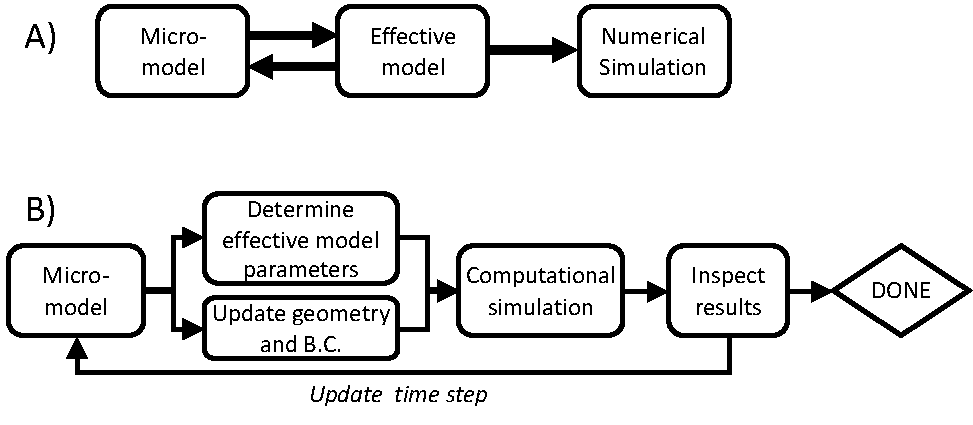
\includegraphics[width=6.5in]{Figures/simulationframework}
\caption{Proposed frame work for using an effective constitutive model to improve the efficiency of using complex meso- or multi-scale models (micro-models) in numerical simulations. Here, A) effective constitutive models act as an intermediate step between micro-models and numerical simulations, where micro-models inform the changes to the effective constitutive model while the effective constitutive model for the simulation. B) An example of how this may be implemented for time-evolving is shown.}
\label{fig:simulationframework}
\end{figure}
%-------------------	 end FIGURE 	-------------------%
%%%%%%%%%%%%%%%%%%%%%%%%%%%%%%%%%%%%%%%%%%%%%%%%%%%%%%%%%%%%
    
    
    
    
    
    
    
    


%-----------------------------------------------------------
%	Constitutive Modeling
%-----------------------------------------------------------

%-------------------	kinematics		-------------------%
%%%%%%%%%%%%%%%%%%%%%%%%%%%%%%%%%%%%%%%%%%%%%%%%%%%%%%%%%%%%%
%%	Constitutive model form									%
%%%%%%%%%%%%%%%%%%%%%%%%%%%%%%%%%%%%%%%%%%%%%%%%%%%%%%%%%%%%%

\section{Effective constitutive model formulation}

%-----------------------------------------------------------
%	Kinematics
%-----------------------------------------------------------
\subsection{Kinematic considerations}
	
	To formulate any soft tissue constitutive model, the choice for kinematic basis is the first step. The choice of kinematic basis has significant impact on the constitutive model form, model parameter covariance, number of parameters necessary and even the quality of fit for parameter estimation. There are two categories for selecting the kinematic basis.
	
\begin{enumerate}
\item Invariants
\item Finite deformation strain tensors
\end{enumerate}

\subsubsection{Invariants} \label{sec:invariants}
%-------	Possible invariants	-------%
	Using invariants is a common choice, which are scalar functions of the right or left Cauchy Green tensor which are independent of rigid body motion. Each invariant describes a facet of deformation: isotropic, volumetric strain, anisotropic, or interactions between them. The breadth of choices, allows for more freedom in selecting a combination of invariants for constitutive models that best describes the mechanisms in the tissue. The three isotropic invariants of the right Cauchy Green tensor are $I_1 = Tr(\mathbf{C})$, $I_2 = \frac{1}{2}\left( Tr(\mathbf{C})^2 - Tr(\mathbf{C}^2)\right)$, $I_3 = \det(\mathbf{C})$. The extension for anisotropic materials is summarized by Holzapfel \cite{holzapfel_nonlinear_2000}. The usual starting point is $I_4 = \mathbf{m}\cdot \mathbf{C} \mathbf{m}$, where $\mathbf{m}$ is a unit vector for material axis, or the preferred direction, most commonly that of the constituent fibers, such as collagen and elastin. Other pseudo invariants include $I_5 = \mathbf{m}\cdot \mathbf{C}^2 \mathbf{m}$, $I_6$ and $I_7$ which are equivalent of $I_4$ and $I_5$ for another family of fibers along some $\mathbf{n}$, $I_8 = \mathbf{m}\cdot\mathbf{C}\mathbf{n}$ and $I_9 = (\mathbf{m}\cdot\mathbf{n})^2$ can be used to describe the interaction between these two fiber families \cite{sacks_novel_2016}\cite{avazmohammadi_novel_2017}, etc. Optimal choice for the invariants can help with parameter estimation by reducing the number of parameters needed. 


%-------	Why traditional invariants are not suitable	-------%	
	However, the use of invariants do not lend itself to creating a single generalized form. For example, there is no specific set of invariants and pseudo invariants that can cover all forms of material behavior of interactions. Including all such invariants, will only lead to an unmanageable number of parameters. One example is when modeling the effects of fiber rotation in tissues with widely distributed fiber orientations. This is one of the most difficult behavior to model using phenomenological approaches. Fiber rotation manifests as coupling interactions between axial stretches in the mechanical response of soft tissues. Invariant based models cannot easily reproduce this effect. One approach is to use the Driessen model \cite{driessen_structural_2005}, where additional fiber families are added until it can match the response of the soft tissue. However, this significantly increases computational costs and requires two additional parameters for each additional fiber family. The number of fiber families needed and their orientations also cannot be generalized. Further extensions to this approach is to incorporate the fiber orientation distribution directly, such as in meso-scale structural approaches \cite{sacks_incorporation_2003a, fata_insights_2014, zhang_meso_2016}. However, this also increases the complexity and computational cost of the model, which defeats the point of phenomenological approaches entirely. Adding coupling invariants such as $I_8$ and $I_9$ are also an option. However, the inherent similarities between these invariants makes it difficult to incorporate them all in a generalized constitutive model form. 
    
    
    
\subsubsection{Conventional finite deformation strain tensors} \label{sec:straintensor}

	The components of strain tensors, such as the Green-Lagrange, $\mathbf{E}$, right Cauchy-Green, $\mathbf{C}$, left Cauchy-Green, $\mathbf{B}$, or the right stretch, $\mathbf{U}$ can be used directly in the constitutive model. One example using strain tensor components is the commonly used generalized Fung model \cite{fung_biomechanics_1993}. The effects of choice of strain tensor is not entirely clearly. Specifically, $\mathbf{U}$ scales linear with the deformation, whereas $\mathbf{E}$, $\mathbf{C}$, and $\mathbf{B}$ scales quadratically with the deformation. Functionally, these tensors behave very similarly. For example, $\mathbf{E}$ is just $\mathbf{C}$ scaled by $1/2$. More often than not, the choice is to simply default to $\mathbf{E}$, which leads to a simple mathematical form for the stress-strain relationship and the elasticity tensor. Although, it is common to use the componential of $\mathbf{E}$ directly, it can be helpful express them with respect to the material axis, $\left[\mathbf{E}\right]_{\mathbf{m}_0,\mathbf{n}_0}$, so that it is not dependent on the specimen orientation or the coordinate system. That is 
\begin{equation} \label{eqn:greenstrain}
E_m = \mathbf{m}_0\cdot\mathbf{E}\mathbf{m}_0, \quad E_n = \mathbf{n}_0\cdot\mathbf{E}\mathbf{n}_0, \quad E_{\phi} = \mathbf{m}_0\cdot\mathbf{E}\mathbf{n}_0,
\end{equation} 
should be used to formulate the constitutive model.

%-------	Hencky strains		-------%

    One additional strain basis we have considered is the Hencky strains, which is the logarithmic strain calculated from the upper triangular decomposition of the deformation gradient tensor with respect to the material axis as described in Criscione \textit{et al.} \cite{criscione_experimentally_2003a} and then further expanded on by Srinivasa \cite{srinivasa_use_2012} and Freed \cite{freed_logarithmic_2015, freed_conjugate_2017, erel_stress/strain_2017}. This has the following number of advantages: (1) The decomposed strains are easy to interpret physically, (2) it results in an extremely simple mathematical form the Cauchy stress, (3) the logarithmic strains are beneficial when dealing with experimental errors in reference configurations, and (4) It is expected to be slightly less correlated in comparison to the Green Lagrange strains. The Hencky strains have the greatest in difference compared to the Green-Lagrange strains, and are thus a good choice for comparing the strain bases.
    
    
%%%%%%%%%%%%%%%%%%%%%%%%%%%%%%%%%%%%%%%%%%%%%%%%%%%%%%%%%%%%
%-------------------	begin FIGURE 	-------------------%
\begin{figure}
\centering
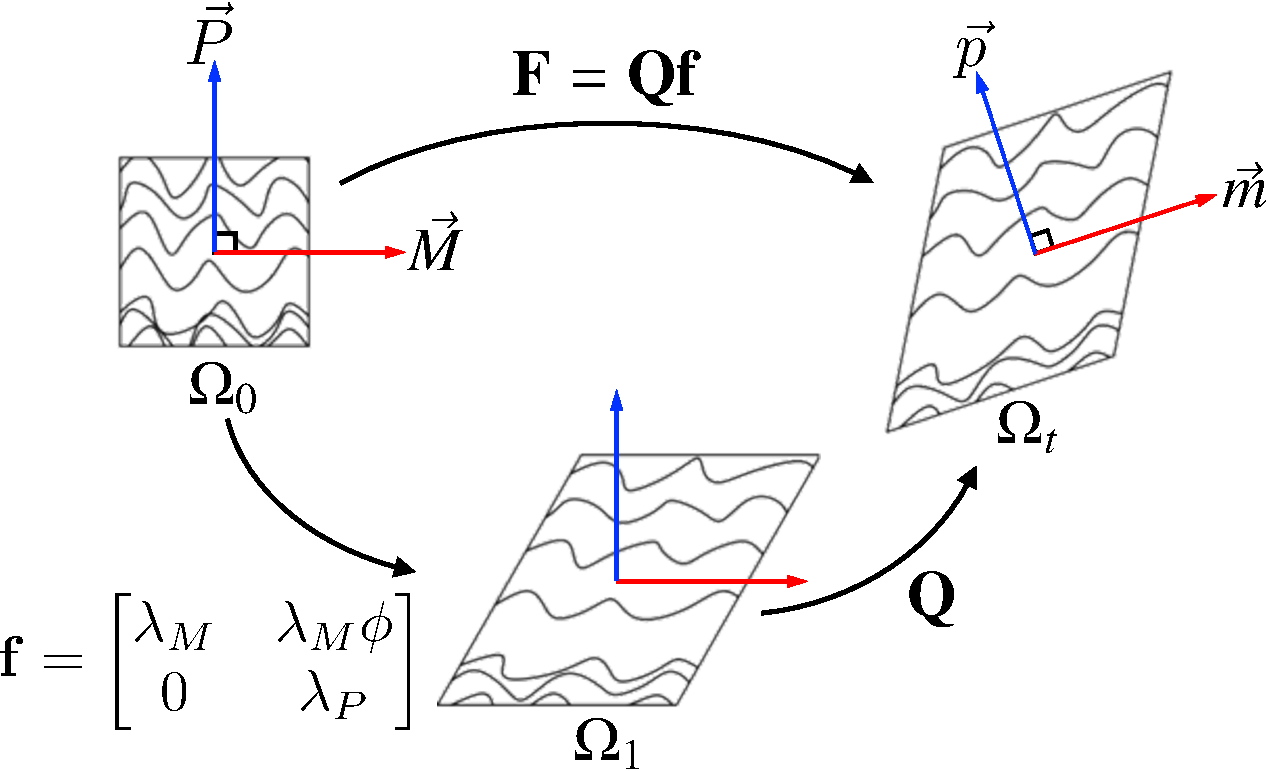
\includegraphics[width=5in]{Figures/henckykinematics}
\caption{The upper triangular decomposition of the deformation gradient tensor with respect the preferred material axis of soft tissues, whose components are used to define the Hencky strains.}
\label{fig:henckykinematics}
\end{figure}
%-------------------	 end FIGURE 	-------------------%
%%%%%%%%%%%%%%%%%%%%%%%%%%%%%%%%%%%%%%%%%%%%%%%%%%%%%%%%%%%%
    
    
    The Hencky strains can be formulated as followed. Briefly, the upper triangular decomposition, $\mathbf{f}$, when expressed with respect to the material axis of the tissue is given by
%==========================================================%
%-------------------	begin EQUATION 	-------------------%
\begin{equation}
\begin{aligned}
\left[\mathbf{f}\right]_{\mathbf{m}_0,\mathbf{n}_0} = \begin{bmatrix}
\lambda_m 	& \lambda_m\phi \\
0			& \lambda_n
\end{bmatrix}.
\end{aligned}\label{eqn:uppertriangulardecomposition}
\end{equation}
%-------------------	 end EQUATION 	-------------------%
%==========================================================%
Here, $\mathbf{m}_0$ is the material axis in the referential configuration, which is generally the preferred direction of the fibers embedded in the tissue, $\mathbf{n}_0$ is the direction perpendicular to $\mathbf{m}_0$, $\mathbf{m}_t$ is the material axis in the deformed configuration, $\mathbf{n}_t$ is the direction perpendicular to $\mathbf{m}_t$, $\lambda_m$ and $\lambda_n$ are the stretches along these axes respectively, and $\phi$ is the angle of shear between $\mathbf{m}_0$ and $\mathbf{n}_0$. The corresponding deformation gradient tensor can thus be expressed as 
%==========================================================%
%-------------------	begin EQUATION 	-------------------%
\begin{equation}
\begin{aligned}
\mathbf{F} = \lambda_m\mathbf{m}_t\otimes\mathbf{m}_0 + \lambda_m\phi\mathbf{m}_t\otimes\mathbf{n}_0 + \lambda_n\mathbf{n}_t\otimes\mathbf{n}_0.
\end{aligned}
\end{equation}
%-------------------	 end EQUATION 	-------------------%
%==========================================================%
The Hencky strains ($\gamma_1, \gamma_2, \gamma_3$), which are functions of the components of $\mathbf{f}$, can be determined using, 
%==========================================================%
%-------------------	begin EQUATION 	-------------------%
\begin{subequations}\label{eqn:henckystrains}
\begin{align}
\gamma_1 &= \log(\lambda_m), &	\gamma_2 &= \log(\lambda_n), 	& \gamma_3 &= \phi	\\
\lambda_m &= \mathbf{m}_t\cdot\mathbf{F}\mathbf{m}_0, &	\lambda_n &= \mathbf{n}_t\cdot\mathbf{F}\mathbf{n}_0,	&	\phi &= \left(\mathbf{m}_t\cdot\mathbf{F}\mathbf{m}_0\right)^{-1}\mathbf{m}_t\cdot\mathbf{F}\mathbf{n}_0.
\end{align}
\end{subequations}
%-------------------	 end EQUATION 	-------------------%
%==========================================================%
    
    
%-------	Hencky vs. Green-Lagrange strain	-------%

	We are most interested in the difference between Green-Lagrange and the Hencky strains for the formulation of the effective constitutive model (Summary Table \ref{tb:greenvshencky}). Firstly, as stated above , Hencky strains lead to a very convenient form for the Cauchy stresses,
%==========================================================%
%-------------------	begin EQUATION 	-------------------%
\begin{equation}\label{eqn:cauchystressform}
\mathbf{T}	= \frac{1}{J} \dpd{\Psi}{\gamma_1} \mathbf{m}_t\otimes\mathbf{m}_t 
			+ \frac{1}{J} \dpd{\Psi}{\gamma_2} \mathbf{n}_t\otimes\mathbf{n}_t 
			+ \frac{\lambda_n}{J\lambda_m} \dpd{\Psi}{\gamma_3} \left(\mathbf{m}_t\otimes\mathbf{n}_t + \mathbf{n}_t\otimes\mathbf{m}_t \right).
%\\
%\dpd{\Psi}{\gamma_1} 	= J \mathbf{m}\cdot\mathbf{T}\mathbf{m}, \quad 
%\dpd{\Psi}{\gamma_2} 	= J \mathbf{s}\cdot\mathbf{T}\mathbf{s}, \quad 
%\dpd{\Psi}{\gamma_3} 	= J \frac{\lambda_m}{\lambda_n}\mathbf{m}\cdot\mathbf{T}\mathbf{s}.
\end{equation}
%-------------------	 end EQUATION 	-------------------%
%==========================================================%
where $\Psi$ is the strain energy density function.
In comparison, the 2nd Piola Kirchhoff stress with Green-Lagrange strains is,
%==========================================================%
%-------------------	begin EQUATION 	-------------------%
\begin{equation} \label{eqn:2ndpkstressform}
\mathbf{S} = \dpd{\Psi}{E_m}\mathbf{m}_0\otimes\mathbf{m}_0
+ \dpd{\Psi}{E_n}\mathbf{n}_0\otimes\mathbf{n}_0 
+ \frac{1}{2}\dpd{\Psi}{E_{\phi}}\left(\mathbf{m}_0\otimes\mathbf{n}_0 + \mathbf{n}_0\otimes\mathbf{m}_0\right),
\end{equation}
%-------------------	 end EQUATION 	-------------------%
%==========================================================%
with the Cauchy stress obtained from push forward, $\mathbf{T} = (1/J) \mathbf{F}\mathbf{S}\mathbf{F}^\mathsf{T}$. Expressing the Green-Lagrange strain with respect to the material axis, ${E_m, E_n, E_\phi}$, is preferred, so that the model parameters are invariant with respect to rigid body motion and changes in the reference coordinate system. There isn't a significant advantage to either strain measure here. However, we do note that the partial derivative of Green-Lagrange strain, $\pd{\mathbf{E}}{\mathbf{C}}$ (Eqn. \ref{eqn:partialgreens}), is much simpler than that of the Hencky strains, $\pd{\gamma}{\mathbf{C}}$ (Eqn. \ref{eqn:henckyderivatives}). As a result, the elasticity tensor, $\mathbb{C} = C_{ijkl}$, for the Hencky strain is much more complex (see Appendix \ref{sec:elasticitytensor}). 

	One other aspect is the difference in correlation between model parameters when using Green-Lagrange strain, $\{E_m, E_n, E_\phi\}$ vs. using Hencky strains $\{\gamma_1, \gamma_2, \gamma_3 \}$. For example, using the for form of the generalized Fung model,
%==========================================================%
%-------------------	begin EQUATION 	-------------------%
\begin{subequations} \label{eqn:generalizedfungmodel}
\begin{align}
\Psi 	&= c_0 \left(e^{Q} - 1\right),\notag \\
\mathrm{with}	\qquad	Q	&= b_1 E_m^2 + b_2 E_n^2 + b_3 E_\phi^2 + 2 b_4 E_m E_n + 2 b_5 E_mE_\phi + 2 b_6 E_nE_\phi	\label{eqn:generalizedfungmodela} \\ 
\mathrm{or}		\qquad	Q	&= b_1 \gamma_1^2 + b_2 \gamma_2^2 + b_3 \gamma_3^2 + 2 b_4 \gamma_1\gamma_2 + 2 b_5 \gamma_1\gamma_3 + 2 b_6 \gamma_2\gamma_3	\label{eqn:generalizedfungmodelb} 
\end{align}
\end{subequations}
%-------------------	 end EQUATION 	-------------------%
%==========================================================%
we compared these two strain basis by computing the correlation matrix between the parameters $b_1$ to $b_6$ for the mechanical data acquired from an exogenously cross-linked bovine pericardium specimen \cite{sun_response_2004} (Appendix \ref{sec:parametercorrelation}). The only difference is that we replaced Green Lagrange strain, $E_m$, $E_n$, $E_\phi$ (Eqn. \ref{eqn:generalizedfungmodela}), with the corresponding Hencky strains $\gamma_1$, $\gamma_2$, $\gamma_3$ (Eqn. \ref{eqn:generalizedfungmodelb}) in the model. The correlation between the parameters are mostly similar in both cases, but the Hencky strains come on top with slightly lower correlations, and the determinant of the correlation matrix is higher, $9.38\times10^{-3}$, in comparison to using the Green Lagrange strains, $7.13\times10^{-3}$, (Fig. \ref{fig:gvsecorrelation}, Appendix \ref{sec:parametercorrelation} Table \ref{tb:correlationE} \& \ref{tb:correlationG}). 



%%%%%%%%%%%%%%%%%%%%%%%%%%%%%%%%%%%%%%%%%%%%%%%%%%%%%%%%%%%%
%-------------------	begin FIGURE 	-------------------%
\begin{figure}
\centering
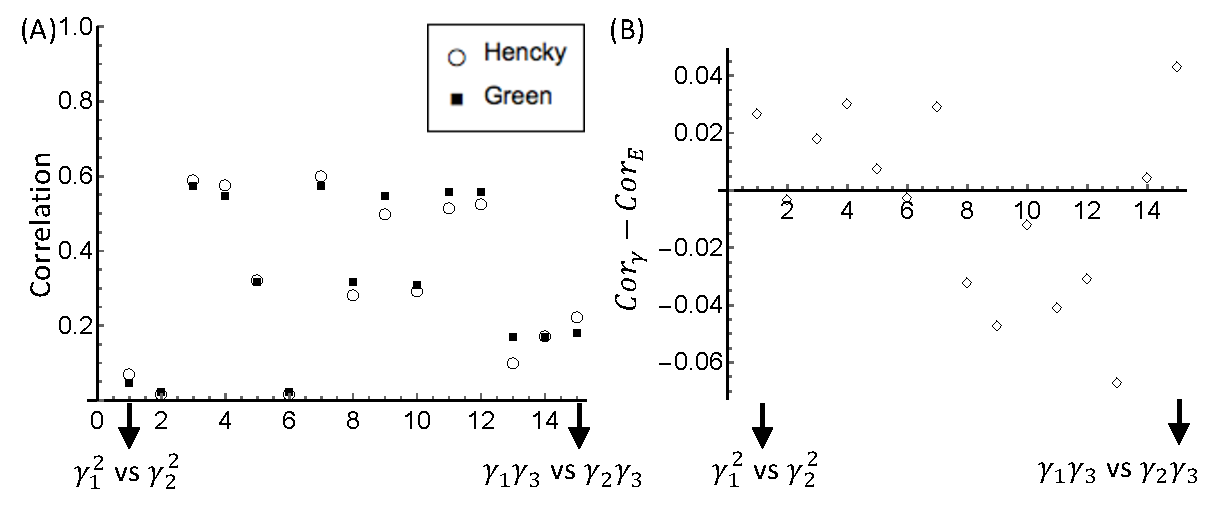
\includegraphics[width=6.5in]{Figures/gvsecorrelation}
\caption{(A) The correlation between parameters pairs in the generalized Fung model when using Green-Lagrange vs Hencky strains. (B) The difference in correlation between each pair of parameters, which is very small but with the Hencky strains being lower overall.}
\label{fig:gvsecorrelation}
\end{figure}
%-------------------	 end FIGURE 	-------------------%
%%%%%%%%%%%%%%%%%%%%%%%%%%%%%%%%%%%%%%%%%%%%%%%%%%%%%%%%%%%%

    
    The last and most important difference between Green-Lagrange and Hencky strains is that they handle compression very differently. Models using Hencky strains tend to increase exponentially under compression, in comparison to models using the Green-Lagrange strains, which only increase mildly with compression. We illustrated this again using the generalized Fung model (Eqn. \ref{eqn:generalizedfungmodel}), with Green-Lagrange or Hencky strain as the input variable (Fig. \ref{fig:gvsecompression}). The reason for this is actually fairly simple, Green-Lagrange strain maps deformations from $\mathbf{E}: [0,\infty] \rightarrow [-1/2,\infty]$, while Hencky strains maps deformations from $\mathbf{\gamma}: [0,\infty] \rightarrow [-\infty,\infty]$, drastically increasing the magnitude of the same strain value under compression. This is problematic, as soft tissues generally behaves very differently under compression than extension. For example, collagen fibers are the most important structural bearing component of most soft tissue. They straighten under extension, which significantly increases the stiffness of the tissue, but buckle and crimp under compression, which does not play a significant role in load bearing \cite{soares_mathematical_2017}. \emph{The behavior of Green-Lagrange strain tensor matches more closely to that of soft tissues}. Due to all factors considered (Table \ref{tb:greenvshencky}), we proceed to use the Green-Lagrange strain tensor as the best kinematic basis to formulate the effective constitutive model. 
    
    
%%%%%%%%%%%%%%%%%%%%%%%%%%%%%%%%%%%%%%%%%%%%%%%%%%%%%%%%%%%%
%-------------------	begin FIGURE 	-------------------%
\begin{figure}
\centering
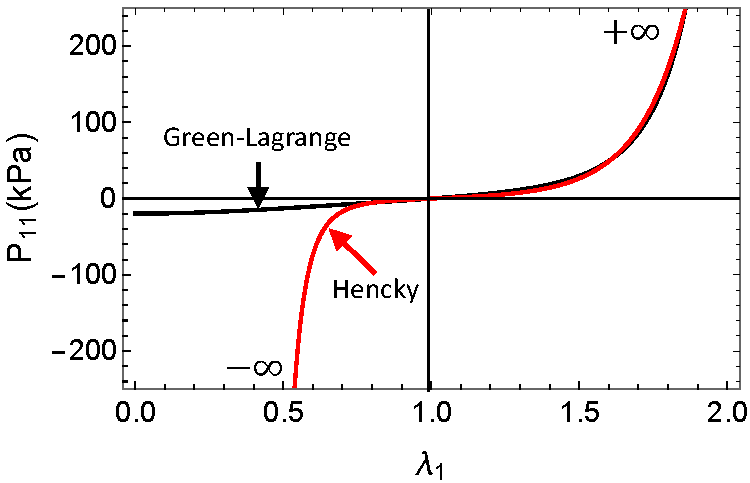
\includegraphics[width=3.25in]{Figures/gvsecompression}
\caption{The response of a generalized Fung model when using Green-Lagrange (Black) vs Hencky strains(Red). Both models are able to match extensional response nearly perfectly with respect to each other, but drastically differ in response under compression.}
\label{fig:gvsecompression}
\end{figure}
%-------------------	 end FIGURE 	-------------------%
%%%%%%%%%%%%%%%%%%%%%%%%%%%%%%%%%%%%%%%%%%%%%%%%%%%%%%%%%%%%


	





%----------------------------------------------------------%
%-------------------	begin TABLE 	-------------------%
\begin{table}
\caption{The difference between using the Green-Lagrange strain tensor versus the Hencky strains to formulate constitutive models. \textbf{Bold} text indicates key advantages and \textit{Italic} text indicate key disadvantages.}
\begin{center}
\label{tb:greenvshencky}
\begin{tabular}{|p{0.9in}|p{2.4in}|p{2.4in}|}
\hline
\rowcolor{Gray}
\multicolumn{1}{|>{\centering\arraybackslash}m{0.9in}|}{Characteristics} 
	& \multicolumn{1}{|>{\centering\arraybackslash}m{2.4in}|}{\textbf{Green-Lagrange strain}} 
    & \multicolumn{1}{|>{\centering\arraybackslash}m{2.4in}|}{\textbf{Hencky strain}}\\
\hline
General & Most commonly used in modeling	& \textbf{Easy to interpret physically} \\
\hline
Stress 	& Even simpler form for the 2nd Piola Kirchhoff stress 
\begin{equation*}
\begin{aligned}
\mathbf{S} =& \dpd{\Psi}{E_m}\mathbf{m}_0\otimes\mathbf{m}_0 + \dpd{\Psi}{E_n}\mathbf{n}_0\otimes\mathbf{n}_0 \\&+ \frac{1}{2}\dpd{\Psi}{E_{\phi}}\left(\mathbf{m}_0\otimes\mathbf{n}_0+\mathbf{n}_0\otimes\mathbf{m}_0\right)
\end{aligned}
\end{equation*}
\normalsize
	& Simple form for the Cauchy stress	%\footnotesize
\begin{equation*}
\begin{aligned}
\mathbf{T} =& \dpd{\Psi}{\gamma_{1}}\mathbf{m}_t\otimes\mathbf{m}_t + \dpd{\Psi}{\gamma_{2}}\mathbf{n}_t\otimes\mathbf{n}_t \\ &+ \frac{\lambda_n}{\lambda_m}\dpd{\Psi}{\gamma_{3}}\left(\mathbf{m}_t\otimes\mathbf{n}_t+\mathbf{n}_t\otimes\mathbf{m}_t\right)
\end{aligned}
\end{equation*}
\normalsize
\\
\hline
\multicolumn{1}{|>{\raggedright}m{0.9in}|}{Elasticity tensor} & \textbf{Much simpler form for the elasticity tensor}
	& \textit{The equations for the elasticity tensor is extremely long} \\
\hline
\multicolumn{1}{|>{\raggedright}m{0.9in}|}{Parameter covariance} 	& 	& \textbf{Modestly less correlation between parameters} \\
\hline
\multicolumn{1}{|>{\raggedright}m{0.9in}|}{Response under compression}	&	\textbf{Modest changes in stress under compression, behaves much more similar to soft tissues due to collagen fiber crimp}
	& \textit{Behaves badly under large compression} \begin{itemize}
	\item Log scaling cause the strain energy to increase exponentially with compression
	\end{itemize}\\
\hline
\end{tabular}
\end{center}
\end{table}
%-------------------	 end TABLE 		-------------------%
%----------------------------------------------------------%

	














%---------------	generalized model form	---------------%
%-----------------------------------------------------------
%	Model formulation
%-----------------------------------------------------------
\subsection{Effective constitutive model form}
\subsubsection{Choosing the family of forms for effective constitutive model}

	To select the specific form, we will take the following key aspects into consideration:
\begin{enumerate}
\item Ability to accurately reproduce the response of a wide range of soft tissues and a wide range of deformations using the same form
\item Minimal number of parameters necessary
\item Minimal covariance between parameters
\item Minimal number of and computational cost of the constraints for convexity
\item Minimal computational demand
\end{enumerate}

    Using phenomenological approaches is necessary due to computational cost. The form of phenomenogical models for soft tissues generally falls into three families. The first family is composed of a summation of polynomials, 
%==========================================================%
%-------------------	begin EQUATION 	-------------------%
\begin{equation}
\begin{aligned}
\Psi	&= \sum_i\sum_j\sum_k c_{ijk}E_m^i E_n^j E_\phi^k. 
\end{aligned} \label{eqn:polynomialmodelform}
\end{equation}
%-------------------	 end EQUATION 	-------------------%
%==========================================================%
We will refer to this family as the polynomial series approach. The second family is composed of separated exponential functions of individual or combinations of invariants or strains used, for example by Vito \textit{et al.} \cite{vito_mechanical_1980},
%==========================================================%
%-------------------	begin EQUATION 	-------------------%
\begin{align}\label{eqn:vitomodelforms}
\Psi 	&= \sum_i\sum_j\sum_k c_{ijk} e^{b_{ijk}E_m^i E_n^j E_\phi^k}.
\end{align}
%-------------------	 end EQUATION 	-------------------%
%==========================================================%
We will refer to this family as the separated exponential approach. The final family is exponential models composed of a single exponential function of the sum of polynomials,
%==========================================================%
%-------------------	begin EQUATION 	-------------------%
\begin{equation}
\begin{aligned}\label{eqn:exponentialmodelform}
\Psi 	&= c_0 \left(e^{Q} - 1\right) \\
Q		&= \sum_i\sum_j\sum_k b_{ijk}E_m^i E_n^j E_\phi^k.
\end{aligned}
\end{equation}
%-------------------	 end EQUATION 	-------------------%
%==========================================================%
and we will refer to this family as the single exponential approach. 


\subsubsection{Generalized effective constitutive model form determination} \label{sec:possibleforms}

	Each approach (Eqn. \ref{eqn:polynomialmodelform}-\ref{eqn:exponentialmodelform}) has its own advantages and disadvantages. Polynomial series approach has the most flexibility. With sufficient number of terms, it can match any response perfectly, like Taylor series expansion. However, this family also requires large number of parameters, making parameter estimation and enforcing convexity very difficult. Polynomial series family is only convex in a specific range, extrapolating outside of this region is extremely unreliable. Even enforcing ellipticity and convexity inside of this region is actually much more costly than parameter estimation itself. The constrained optimization problem is not well pose. There are too many constraints and parameters that result in many local minima near or just outside of constrained region. No specific set of parameters are necessarily correct or better, but the objective function values are very similar. This leads to slow convergence and difficulties for most gradient based algorithms. As such, the polynomial series approach is not suitable for the effective constitutive model due to the slow parameter estimation. 


	The separated exponential approach generally suffers from the same issues as the polynomial series. This model form behaves like polynomial series with variable exponents, i.e. $c_1e^{b_1E_m} = c_1y^{b_1}$, where $y =e^{E_m}$. The advantage of this family of models is that similar and highly covariant terms such as $c_1 E_m + c_2 E_m^2 + c_3 E_m^3 ...$ can be avoided, reducing the number of parameters needed. However, like the polynomial series family, coupling terms such as $c_4 e^{b_4 E_m E_n}$ are not convex or elliptical functions, resulting in the same issues for parameter estimation and enforcing convexity. The number of parameters required to fully reproduce the mechanical response is still quite large. Moreover, for the same number of parameters, the separated exponential form is woefully insufficient at reproducing the mechanical response of soft tissues in comparison to the single exponential approach. As such, the advantages gained is actually quite minimal. 
    
    
    The single exponential approach has substantial parameter covariance, but is extremely effective at reproducing the response of soft tissues using a small number of parameters, is computationally efficient, and is easy to enforce convexity for. Because exponential function is monotonically increasing, enforcing convexity and ellipticity only requires the polynomial $Q$ to be convex and elliptical. This is the best balance for our goals (end of Section \ref{sec:straintensor}), and is thus our choice for the effective constitutive model. The first step is of course to examine the generalized Fung model (Eqn. \ref{eqn:exponentialmodelform}). We find that the generalized Fung model is not able to fully reproduce the mechanical response of pericardium and aortic valve tissues, it can only do so in a limited range. Although this is enough for most numerical simulations, where the deformations are generally limited to the physiologic range, it is not always sufficient for predicting the mechanical response when organs undergo significant changes in geometry, causing the deformations to change drastically. The easiest way to visualize this is through contour plots of the strain energy function (Fig. \ref{fig:strainenergycontours}). The mechanical response of soft tissues general has hyperelliptical contours (Fig. \ref{fig:strainenergycontours}A), whereas the generalized Fung model always has precisely elliptical contours (Fig. \ref{fig:strainenergycontours}B), which has some advantages. Ellipticity and convexity is very easy to guarantee, and the elasticity tensor and behavior at small strains is easy to derive. However, when the range of deformation is sufficiently large, the contours of the generalized Fung model essentially stretches and rotates to match the soft tissue to the best of its abilities (Fig. \ref{fig:strainenergycontours}B), but is not able to fully reproduce the resulting tissue response. It can only serve as an approximation.  


%%%%%%%%%%%%%%%%%%%%%%%%%%%%%%%%%%%%%%%%%%%%%%%%%%%%%%%%%%%%
%-------------------	begin FIGURE 	-------------------%
\begin{figure}
\centering
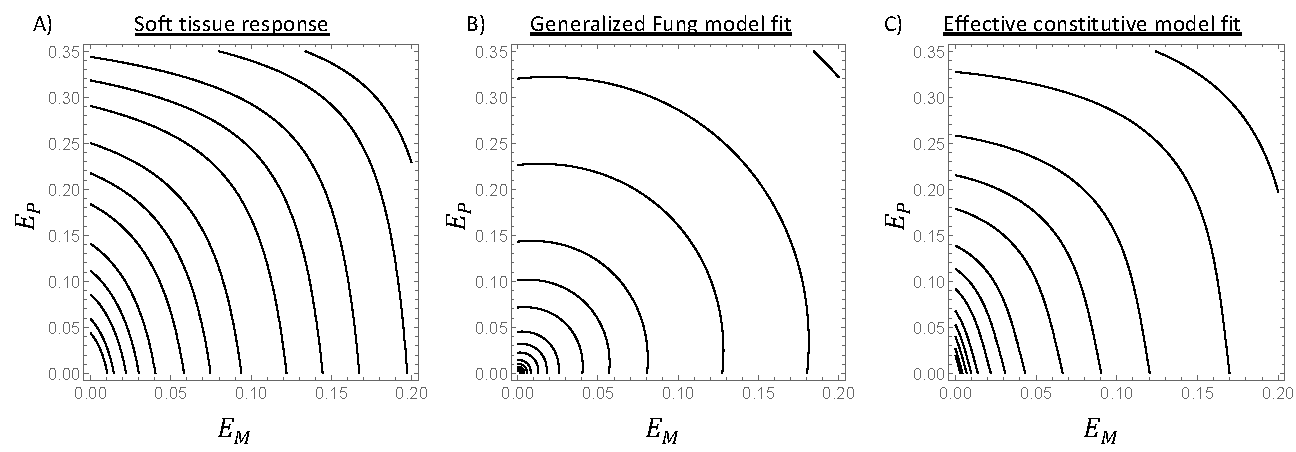
\includegraphics[width=6.5in]{Figures/strainenergycontours}
\caption{The contour plots of strain energy (kPa) of A) a bovine pericardial specimen using a meso-scale structural model \cite{zhang_modeling_2017}, B) best fit using the generalized Fung model (Eqn. \ref{eqn:generalizedfungmodel}), and C) best fit using the effective constitutive model we develop from herein showing the necessity of extending existence phenomenological model form.}
\label{fig:strainenergycontours}
\end{figure}
%-------------------	 end FIGURE 	-------------------%
%%%%%%%%%%%%%%%%%%%%%%%%%%%%%%%%%%%%%%%%%%%%%%%%%%%%%%%%%%%%

\subsubsection{Final effective material model form} \label{sec:finalform}

	Thus, for our effective constitutive model, we extended the polynomial $Q$ one step further, allowing hyperellipticity of the strain energy density function (Fig. \ref{fig:strainenergycontours}C). For the additional terms to include, we move up to the next even powers, up to the quartic terms (exponents $i+j+k\leq4$) (Eqn. \ref{eqn:exponentialmodelform}), as odd numbered powers do not yield elliptical functions. 
% The most generalized form possible is 
% %==========================================================%
% %-------------------	begin EQUATION 	-------------------%
% \begin{equation}
% \begin{aligned}\label{eqn:fullgeneralizeexponentialform}
% \Psi 	&= c_0 \left(e^{Q} - 1\right) \\
% Q		&= \sum_i\sum_j\sum_k b_{ijk} E_m^i E_n^j E_\phi^k, \quad  {i+j+k\leq4}.
% \end{aligned}
% \end{equation}
% %-------------------	 end EQUATION 	-------------------%
% %==========================================================%   
There is a total of 34 possible terms in Q. Not all terms are required or even admissible. Specifically, the following constraints are enforced on the model:
      
      \underline{Constraint 1}: \underline{The stress must be zero in the reference configuration}. Given that the stress is the gradient of $\Psi$, where is $\Psi^\prime = c_0 Q^\prime e^Q$, all terms that is non-zero in $Q^\prime$ at zero strain must be zero. This corresponds to all $i+j+k = 1$ terms, leaving 31 terms remaining. 
      
      \underline{Constraint 2}: \underline{The response must be elliptic}, that is the line joining any two point along the strain energy function surface must have positive curvature. Keeping in mind that the generalized Fung model (Eqn. \ref{eqn:exponentialmodelform}) is already close to being sufficient as reproducing the response of many soft tissues we tested. We only want to extend this to be able to reproduce a wide range of soft tissue responses. Furthermore, in considerations of limiting the number of parameters, reducing parameter correlation, non-elliptical terms making constrained optimization much more difficult, and that the non-elliptical terms must be small, we choose to forgo all $i+j+k = 3$ terms, leaving 21 terms remaining. 
      
      \underline{Constraint 3}: \underline{Response must be independent of the direction of shear}. Since we decompose the Green-Lagrange strain relative to the material axis, this creates a plane of symmetry in the soft tissue response for the direction of shear. Thus, the value of $E_\phi$ can only have even powers, $k = 2,4$. The following terms are thus necessarily zero: $E_m^3E_\phi$, $E_m^2E_nE_\phi$, $E_mE_n^2E_\phi$, $E_n^3E_\phi$, $E_mE_\phi^3$, $E_nE_\phi^3$, $E_mE_\phi$, and $E_nE_\phi$. 
      
The final form of the effective constitutive model is thus
%==========================================================%
%-------------------	begin EQUATION 	-------------------%
\begin{equation}
\begin{aligned}\label{eqn:generalizeexponentialform}
\Psi	=& c_0 \left(e^{Q} - 1\right) \\
Q		=& b_1 E_m^2 + b_2 E_n^2 + b_3 E_\phi^2 + b_4 E_m E_n + b_5 E_m^4 + b_6 E_n^4 + b_7 E_m^3 E_n + b_8 E_m^2 E_n^2 + b_9 E_m E_n^3	\\
	&+ b_{10} E_\phi^4 + b_{11} E_m^2E_\phi^2 + b_{12} E_n^2 E_\phi^2 + b_{13} E_m E_n E_\phi^2.
\end{aligned}
\end{equation}
%-------------------	 end EQUATION 	-------------------%
%==========================================================%








%-----------------------------------------------------------
%	Model convexity
%-----------------------------------------------------------
\subsubsection{Convexity and ellipticity}

	Perhaps the biggest advantage of the single exponential approach models is the convenience for enforcing ellipticity and convexity. Because ellipticity and convexity are preserved by monotonically increase functions, such as $e^x$, we only have to enforce ellipticity and convexity of $Q$ (Eqn. \ref{eqn:generalizeexponentialform}). Sylvester's criterion \cite{gilbert_positive_1991}, is the most convenient for constraints in this scenario, which is given by 
%==========================================================%
%-------------------	begin EQUATION 	-------------------%
\begin{equation}\label{eqn:convexitycriteria}
\begin{aligned}
\dpd[2]{Q}{E_m} \geq 0, \quad
\det
\begin{bmatrix}
\dpd[2]{Q}{E_m} & \dmd{Q}{2}{E_m}{}{E_n}{}\\
\dmd{Q}{2}{E_m}{}{E_n}{} & \dpd[2]{Q}{E_n}\\
\end{bmatrix} \geq0, \quad
\det
\begin{bmatrix}
\dpd[2]{Q}{E_m} & \dmd{Q}{2}{E_m}{}{E_n}{} & \dmd{Q}{2}{E_m}{}{E_\phi}{}\\
\dmd{Q}{2}{E_m}{}{E_n}{} & \dpd[2]{Q}{E_n} & \dmd{Q}{2}{E_n}{}{E_\phi}{}\\
\dmd{Q}{2}{E_m}{}{E_\phi}{} & \dmd{Q}{2}{E_n}{}{E_\phi}{} & \dpd[2]{Q}{E_\phi} \\
\end{bmatrix} \geq0.
\end{aligned}
\end{equation}
%-------------------	 end EQUATION 	-------------------%
%==========================================================%
\emph{This condition is also equivalent of strict convexity \cite{ball_strict_1980}}, so both conditions will be satisfied. For the generalized Fung model (Eqn. \ref{eqn:exponentialmodelform}), this simply required that $b_1>0$, $b_1b_2-b_4>0$, and $b_3(b_1b_2 - b_4^2) - b_5(b_2b_5 - b_4b_6) - b_6(b_1b_6 - b_4b5)>0$. Convexity and ellipticity for the effective constitutive model is also simple to enforce. The non-convex region start from a point along the respective axis for each component $E_m$, $E_n$, and $E_\phi$, then spreads out in the shape of a fan as the strain increases depending on which specific coupling terms, such as $E_m^3 E_n$ and $E_m E_n^3$ are present (Fig. \ref{fig:convexitybehavior}). As long as the effective constitutive model is convex on the largest value along the $E_m$, $E_n$, and $E_\phi$ axis respectively, then the effective constitutive model is convex over the entire range. For example, the effective constitutive model is convex if the maximum point on the $E_m$-axis is convex for $E_m^3 E_n$ (Fig. \ref{fig:convexitybehavior}A) or if the maximum point on the $E_n$-axis is convex for $E_m E_n^3$ (Fig. \ref{fig:convexitybehavior}B). Thus, assuming an upper limit of $E_m < 1$, $E_n < 1$, and $E_\phi < 1$, the following constraints on the parameters are sufficient to guarantee convexity and ellipticity,
%==========================================================%
%-------------------	begin EQUATION 	-------------------%
\begin{equation} \label{eqn:effmodelconstraints}
\begin{aligned}
b_1, b_2,b_3,b_5,b_6,b_{10} \geq 0	\\
4(b_1 + 6 b_5) (b_2 + b_8) - (b_4 + 3 b_7)^2 \geq 0		\\
4(b_2 + 6 b_6) (b_1 + b_8) - (b_4 + 3 b_9)^2 \geq 0 	\\
4(b_1 + b_{11}) (b_2 + b_{12}) - (b_{13} + b_4)^2 \geq 0 	\\
b_3+b_{11} \geq 0	\\
b_3+b_{12} \geq 0.	\\
\end{aligned}
\end{equation}
%-------------------	 end EQUATION 	-------------------%
%==========================================================%


%%%%%%%%%%%%%%%%%%%%%%%%%%%%%%%%%%%%%%%%%%%%%%%%%%%%%%%%%%%%
%-------------------	begin FIGURE 	-------------------%
\begin{figure}
\centering
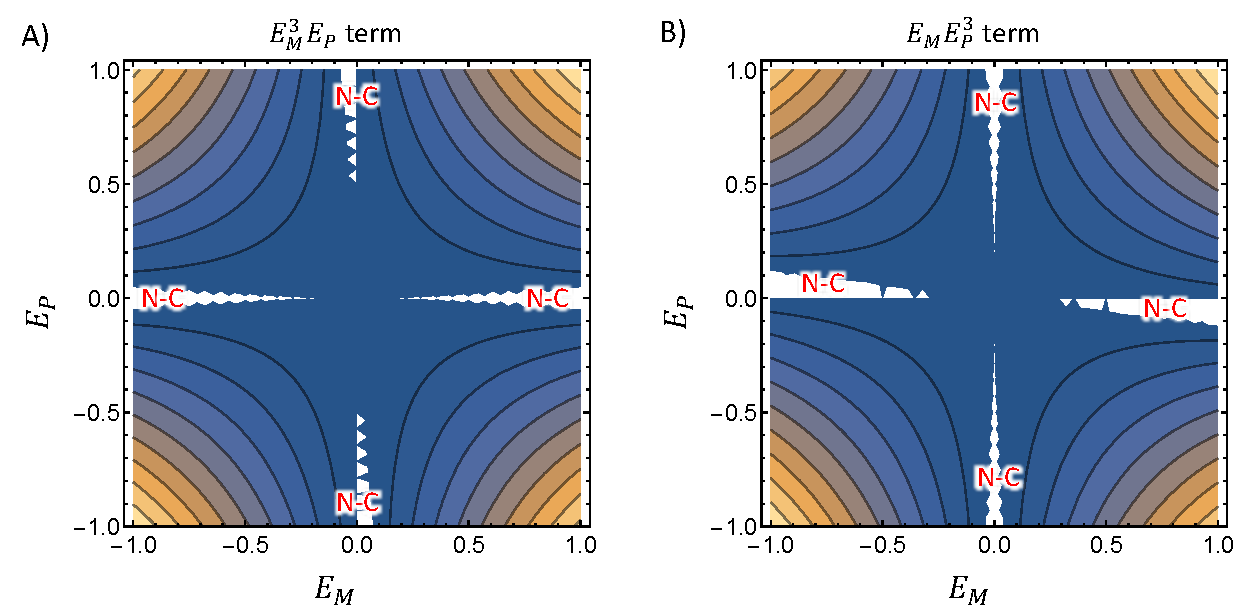
\includegraphics[width=6.5in]{Figures/convexitybehavior}
\caption{The criteria for ellipticity (Eqn. \ref{eqn:convexitycriteria}) plotted against the components of the Green-Lagrange strain for A) when including the $E_m^3E_n$ term and B) $E_mE_n^3$ term. The white regions are not convex (N-C), which start at a point along the axes and spreads out as the strain increases.}
\label{fig:convexitybehavior}
\end{figure}
%-------------------	 end FIGURE 	-------------------%
%%%%%%%%%%%%%%%%%%%%%%%%%%%%%%%%%%%%%%%%%%%%%%%%%%%%%%%%%%%%














%-------------------	scaling			-------------------%
%-----------------------------------------------------------
%	Model scaling for parameter estimation
%-----------------------------------------------------------
\subsection{Model scaling method to improve parameters correlation for parameter estimation} \label{sec:modelscaling}

%-----------------------------------------------------------
%	Computational approaches	
\subsubsection{Parameter correlation for exponential type models}

	One challenging problem with model parameter determination is covariance between the parameters during parameter estimation. Covariance explains how two parameters influence the response of the model and how they will be updated during parameter estimation. High parameter covariance results in both slow convergence and poor reliability and reproducibility of the material parameters. When scaled by the variance of the two parameters, this becomes the correlation between the parameters, with an absolute value between $0$ and $1$. Correlation equal to $1$ implies that two parameters have the exact same effect on the model response, and are thus indistinguishable during parameter estimation. The covariance issue for constitutive models with an exponential function is well described by Aggarwal \cite{aggarwal_inverse_2015, aggarwal_improved_2017}. These constitutive models with exponential functions have a long valley like region in the objective function space. Inside this valley, significantly different parameters produce similar objective function values. This present several problems. 1) It's difficult to compare model parameters between different specimens, because drastically different parameters can produce similar responses. As such, average or representative specimen has little real meaning, and each specimen needs to be fitted individually for simulations. 2) Once trapped in the valley, the convergence of gradient based optimization algorithms becomes excruciatingly slow due to the small gradients while within this valley. 3) The covariance between parameters are extremely large, decreasing the accuracy or in other word increasing the confidence interval of parameters obtaining. 
    
    Aggarwal \textit{et al.} suggested two improvements to alleviate this problem \cite{aggarwal_improved_2017}. These improvements are 1) modifying the modulus parameter $A$ to $e^{a}$, straightening the shape of the valley, and 2) introduce the log-norm for the objective function, improving the gradient along the valley. These modifications have been shown to be effective. However, this is not always ideal. The logarithmic norm suggested faces some issues when fitting stresses or strains, which may be negative and thus becomes undefined. Although this may be alleviated by forgoing data points with negative strains or stresses, but the model may still produce negative values during parameter estimation. Other methods can be used to discard negative values or to take the norm of such values, but these approaches create discontinuities in the gradient of the objective function, causing convergence problems during parameter estimation. Clearly, additional improvements can still be made. 


%-----------------------------------------------------------
%	Scaling method
\subsubsection{Model scaling method}

	We begin by examining the fundamental reason for the high parameter covariance. For this, we will use the 1-D case as an example,
%==========================================================%
%-------------------	begin EQUATION 	-------------------%
\begin{equation}
\begin{aligned}
\Psi &= A \left(e^{B \epsilon} - 1\right) \\
\mathcal{F} &= \sum_i \left(\Psi(\epsilon_i) - \Psi_i \right)^2,
\end{aligned}
\end{equation}
%-------------------	 end EQUATION 	-------------------%
%==========================================================%
where $\Psi$ is the strain energy of our model, $\epsilon$ is some invariant that is a function of the strain, $\epsilon_i$ and $\Psi_i$ are simulated data, and $\mathcal{F}$ is our objective function for parameter estimation. The parameters $A$ and $B$ have different purposes: $A$ is like a modulus, linearly increasing the stiffness of the material, while $B$ modifies the shape of the response, controlling the nonlinearity of the material. However, practically, the two parameters have nearly the same effect on the mechanical response, increasing $A$ increases the stiffness (Fig. \ref{fig:scalingapproach}A) and increasing $B$ also increases the stiffness (Fig. \ref{fig:scalingapproach}B). This is the reason for the high correlation between the parameters (Fig. \ref{fig:scalingapproach}), 0.9979.


%%%%%%%%%%%%%%%%%%%%%%%%%%%%%%%%%%%%%%%%%%%%%%%%%%%%%%%%%%%%
%-------------------	begin FIGURE 	-------------------%
\begin{figure}
\centering
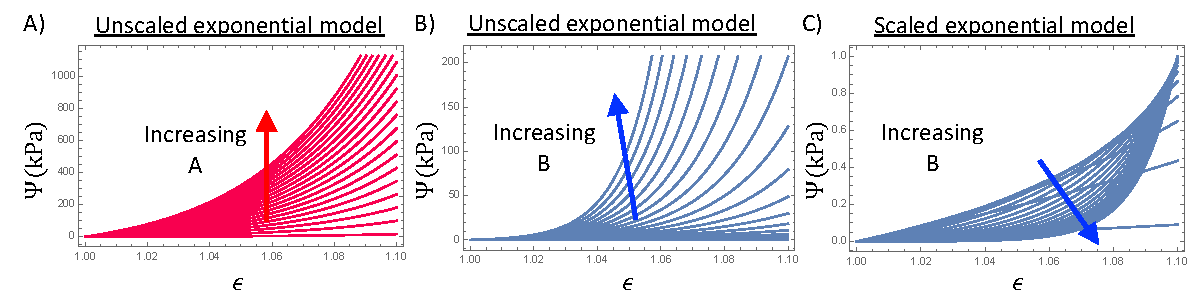
\includegraphics[width=6.5in]{Figures/scalingapproach}
\caption{A)The effect of increasing the values of the modulus $A$ on exponential type models. B) The effect of increasing the values of exponent $B$ on exponential type models, which is very similar to the modulus $A$. C) The effect of increasing the values of parameter $B$ after applying the proposed scaling, increasing the values of parameter $A$ remains the same as in A).}
\label{fig:scalingapproach}
\end{figure}
%-------------------	 end FIGURE 	-------------------%
%%%%%%%%%%%%%%%%%%%%%%%%%%%%%%%%%%%%%%%%%%%%%%%%%%%%%%%%%%%%


	To address this problem, we introduce a scaling term to normalize the exponential part of the model, preventing increasing $B$ from increasing the value of the strain energy as a whole, allowing it to only control the curvature. For this, we will use a value $\epsilon_{max}$, which represents the data point with the maximum strain energy value used for parameter estimation, which is also the point where the strain energy stays the same with changes in $B$. The scaled form is thus given by
%==========================================================%
%-------------------	begin EQUATION 	-------------------%
\begin{equation}
\begin{aligned}
\Psi = \Psi_s = \bar{A} \left[e^{-B\epsilon_{max}} \left( e^{B\epsilon} - 1\right)\right],\label{eqn:scaledmodel1D}
\end{aligned}
\end{equation}
%-------------------	 end EQUATION 	-------------------%
%==========================================================%
where $\bar{A}$ is the scaled version of the modulus $A$. This scaling keeps the exponential part of the model, $e^{-B\epsilon_{max}} ( e^{B\epsilon} - 1)$, at approximately the same value of 1.0 at $\epsilon_{max}$, regardless of the changes in the values of the parameter $B$ (Fig. \ref{fig:scalingapproach}C). This effect is not exact for values of $B < 5$ due to the $-1$ needed to set the strain energy to 0 in the referential configuration, but is nonetheless sufficient for our goal: decoupling the modulus increasing effect of the parameter $A$ from the curvature increasing effect of parameter $B$. Indeed, we found this approach to be successful. We examined the contour plot of the objective function with respect to each of the 4 cases in Aggarwal's work \cite{aggarwal_improved_2017}, with the standard objective function, with $A=e^{a}$, with log-norm, and with $A=e^{a}$ and the log-norm, for both the case without scaling and with scaling (Fig. \ref{fig:objfunctionsurfaces}). First, correlation between the parameters do not change with $A=e^{a}$. The log-norm improves the correlation from 0.9979 to 0.9063(Table \ref{tb:ABcorrelation}), which significantly improves the objective function surface (Fig. \ref{fig:objfunctionsurfaces}). On the other hand, our scaling method improves the correlation from 0.9979 to 0.6186, more significant than using the log-norm. Interestingly, combining scaling and the log-norm has the adverse effect, increasing the correlation back from 0.6186 to 0.8592. This is a result of essentially linearizing the relation between $A$ and $B$, i.e. from $Ae^{B\epsilon}$ to $Log(A)+B\epsilon$, causing the relationship between $A$ and $B$ to go from modulus and nonlinearity to baseline and modulus. Clearly, \emph{the most optimal parameter estimation approach is to use scaling method with no other modifications}. 
    
    
%%%%%%%%%%%%%%%%%%%%%%%%%%%%%%%%%%%%%%%%%%%%%%%%%%%%%%%%%%%%
%-------------------	begin FIGURE 	-------------------%
\begin{figure}
\centering
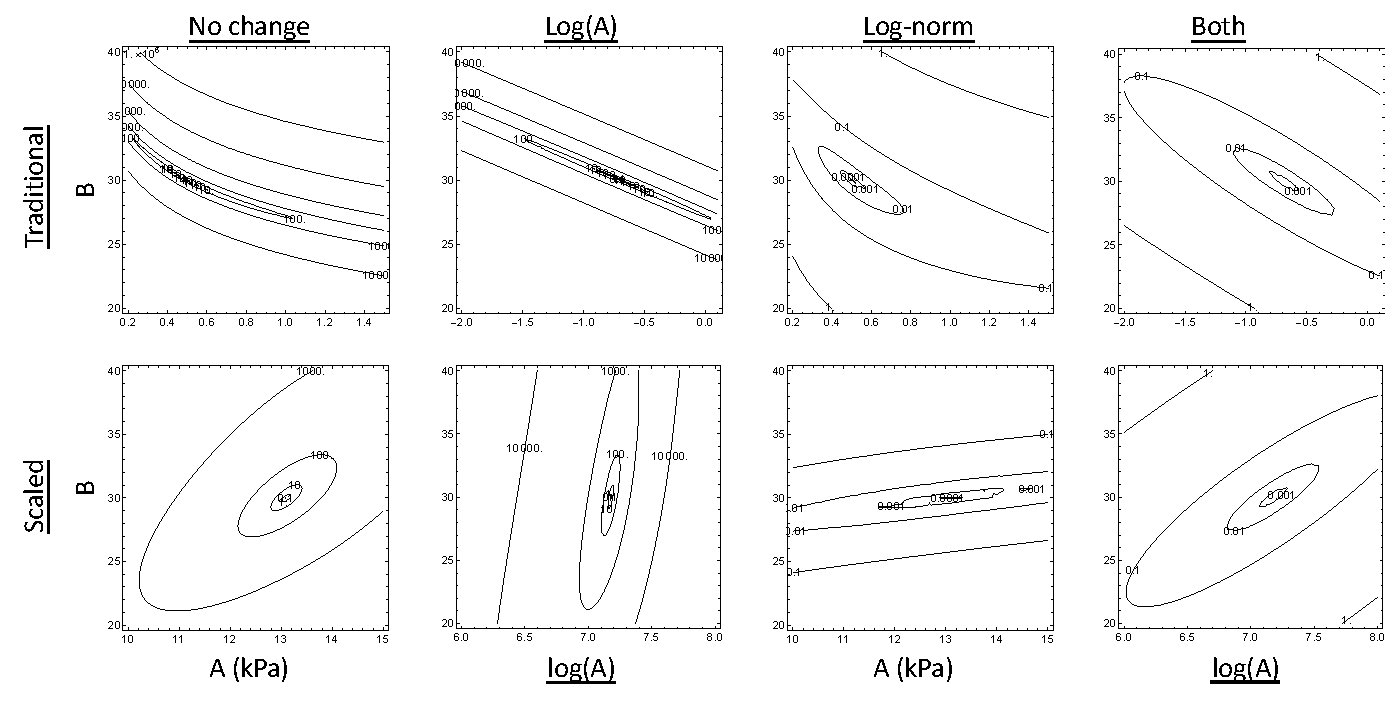
\includegraphics[width=6.5in]{Figures/objfunctionsurfaces}
\caption{(Top) The objective function surface for the traditional unscaled exponential models and (Bottom) objective function surface after scaling. From Left to Right are: the unchanged surface, the surface after changing $A$ to $e^{a}$, using the log-norm for the objective function, and applying both changes. The scaled form with no other changes behaves the best.}
\label{fig:objfunctionsurfaces}
\end{figure} 
%-------------------	 end FIGURE 	-------------------%
%%%%%%%%%%%%%%%%%%%%%%%%%%%%%%%%%%%%%%%%%%%%%%%%%%%%%%%%%%%%


%----------------------------------------------------------%
%-------------------	begin TABLE 	-------------------%
\begin{table}
\caption{The correlation between model parameter when using Hencky strains}
\begin{center}
\label{tb:ABcorrelation}
\begin{tabular}{|l|rrrr|}
\hline
			& No change	& $\log(A)$	& $\log$-norm	& Both \\
\hline
Traditional	& -0.9979	& -0.9979	& -0.9063		& -0.9063 \\
Scaled 		& 0.6186	& 0.6186	& 0.8592		& 0.8592 \\
\hline
\end{tabular}
\end{center}
\end{table}
%-------------------	 end TABLE 		-------------------%
%----------------------------------------------------------%



%-----------------------------------------------------------
%	Relation to unscaled form
% \subsubsection{Relation to unscaled model}

    By design, the value of the exponential parameters $B$ does not change by using the scaling method. Since the scaling term does not depend on the input strain, it acts as a modification to the modulus $A$ while keeping the exponential term the same. This also implies that the relationship between the unscaled modulus $A$ and the scaled modulus $\bar{A}$ is
%==========================================================%
%-------------------	begin EQUATION 	-------------------%
\begin{equation}
\begin{aligned}
A = \bar{A} e^{-B\epsilon_{max}},
\end{aligned}
\end{equation}
%-------------------	 end EQUATION 	-------------------%
%==========================================================%
making finding the actual unscaled parameters a simple task. One other benefit of this scaling approach is that the value of $\bar{A}$ is extremely straight forward and intuitive, it is the strain energy of the model at $\epsilon_{max}$. As a result, the value of $\bar{A}$ can be determined \textit{a priori}, or at the very least very easy to make an initial guess for. This will in turn also help to make parameter estimation faster and more accurate, leaving only the parameter $B$ to be determined. 


%-----------------------------------------------------------
%	Extension to multi-variable form
\subsubsection{Extension to multiple variables}

	Extending this method to multiple variables is very simple. For $\Psi_{eff}$ (Eqn. \ref{eqn:finalmodelform}), the input variables become $\mathbf{\epsilon} = \{E_m, E_n, E_\phi\}$, and $\mathbf{\epsilon}_{max} = \{E_m^{max},E_n^{max},E_\phi^{max}\}$. Determining the values for $\mathbf{\epsilon}_{max}$ depends on the form of the objective function. Using the most common case as the example, which is the sum of the squares of the differences in the 2nd Piola Kirchhoff stress,
%==========================================================%
%-------------------	begin EQUATION 	-------------------%
\begin{equation}
\begin{aligned}
\mathcal{F} = \sum_i \left(S_{11}(\epsilon_i) - \hat{S}_{11}^i\right)^2 + \left(S_{12}(\mathbf{\epsilon}_i) - \hat{S}_{12}^i\right)^2 + \left(S_{22}(\epsilon_i) - \hat{S}_{22}^i\right)^2,
\end{aligned}
\end{equation}
%-------------------	 end EQUATION 	-------------------%
%==========================================================%
$\mathbf{\epsilon}_{max}$ is the data point $\mathbf{\epsilon}_i$ which maximizes $\left(\hat{S}_{11}^i\right)^2 + \left(\hat{S}_{12}^i\right)^2 + \left(\hat{S}_{22}^i\right)^2$. 
Thus, we also introduce a $Q_{max}$ such that,
%==========================================================%
%-------------------	begin EQUATION 	-------------------%
\begin{equation} \label{eqn:finalexponentialmodelformscaled}
\begin{aligned}
\Psi_{eff} 	=& c_0 \left(e^{Q} - 1\right) + \Psi_\mathrm{mat} - p\left(\mathrm{J}-1\right) \\
            =& c_0^\prime e^{-Q_{max}}\left(e^{Q} - 1\right)	
	+ \frac{\eta_M}{2} \left( \frac{1}{\alpha}\left( I_1 -3\right)^{\alpha} + \frac{r}{\beta} \left( I_1 -3\right)^{\beta} \right) - p\left(\mathrm{J}-1\right)\\
Q		=& b_1 E_m^2 + b_2 E_n^2 + b_4 E_m E_n + b_5 E_m^4 + b_6 E_n^4 +
b_9 E_m E_m^3 + b_{10} E_n^4 + b_{11} E_m^2E_\phi^2 + b_{12} E_n^2 E_\phi^2 	\\
Q_{max}	=& b_1 (E_m^{max})^2 + b_2 (E_n^{max})^2 + b_4 E_m^{max} E_n^{max} + b_5 (E_m^{max})^4 + b_6 (E_n^{max})^4 +
b_9 E_m^{max} (E_m^{max})^3 	\\
		&+ b_{10} (E_n^{max})^4 + b_{11} (E_m^{max})^2(E_\phi^{max})^2 + b_{12} (E_n^{max})^2 (E_\phi^{max})^2,
\end{aligned}
\end{equation}
%-------------------	 end EQUATION 	-------------------%
%==========================================================%
where parameter estimation will be done for $c_0^\prime$ instead of $c_0$. Computing the response functions and the stresses, or even the elasticity tensor remains very simple, only requiring multiplying each term by $e^{-Q_{max}}$. Thus, this scaling method is a very simple and easy to implement method of improving the speed and convergence for the parameter estimation of exponential type models. 





%---------------	optimal loading path	---------------%
%-----------------------------------------------------------
%	Optimal loading paths
%-----------------------------------------------------------
\subsection{Optimal \textit{in silico} loading paths for parameter estimation}\label{sec:optimaldesign}

	Another technique for improving the parameter estimation process for determining $\Psi_{eff}$ from respective micro-models is establishing optimal loading paths. An example is the work of Avazmohammadi \cite{Avazmohammadi2017b}, where optimal experimental design is used to 1) minimize the amount of data necessary and 2) improve model parameter covariance for parameter estimation. Just like one of the most important question to ask before performing any mechanical testing is how much and what kind of data is necessary, we should also be selective with our choice of sampling points for parameter estimation. Theory for optimal design of experiment is a well-studied and documented \cite{lanir_optimal_1996, zhu_d_2014}. Vast majority of the methods for optimal design uses D-optimality as the design variable,
%==========================================================%
%-------------------	begin EQUATION 	-------------------%
\begin{equation}\label{eqn:doptimality}
\begin{aligned}
D = \det(\mathbfcal{I}), \quad \mathbfcal{I} = \mathbf{J}^\mathsf{T}\mathbf{J} \quad \mathrm{or} \quad \mathbfcal{I} = \mathbfcal{H},	\\
\mathrm{where} \ J_{ij} = \dpd{f_i}{\xi_j}, \quad \mathcal{H}_{ij} = \dmd{\mathcal{F}}{2}{\xi_i}{}{\xi_j}{},
\end{aligned}
\end{equation}
%-------------------	 end EQUATION 	-------------------%
%==========================================================% 
where $\mathbf{\xi}$ is a vector of model parameters, $\mathbfcal{I}$, the information matrix, can be computed from the derivatives of the objective function $\mathcal{F}$, where $f$ is the model evaluated at each data point, or $\mathbfcal{I}$ can be computed from the Hessian of the objective function, $\mathbfcal{H}$ (Appendix \ref{sec:parametercorrelation}). D-optimality, as the determinant of the information or the hessian matrix at best fit, offers the best representation of both parameter accuracy (parameter covariance or correlation) and precision (parameter variance) at the same time.

    
    The first and foremost step is to establish the parameterization for loading paths so they can be optimized. This is especially important and not straight a forward choice, as the number of loading paths required is not yet established. Another troubling this issue is that because the number of data points are discrete values, the D-optimality is typically not differentiable with respect to the control parameters. For the sake of time spent during optimization, the number of data points is to be kept at the minimal number necessary, thus exacerbating the issue of differentiability. Even worse is perhaps that the optimum is significantly better than the surrounding values, with non-optimal values essentially to zero. Unless the initial guess is near the optimum, optimization is very difficult. This of course means that conventional gradient algorithms are not practical for optimal design, requiring the need for Monte Carlo, random search or divide and conquer strategies, which are much more time consuming. 
    

%%%%%%%%%%%%%%%%%%%%%%%%%%%%%%%%%%%%%%%%%%%%%%%%%%%%%%%%%%%%
%-------------------	begin FIGURE 	-------------------%
\begin{figure}
\centering
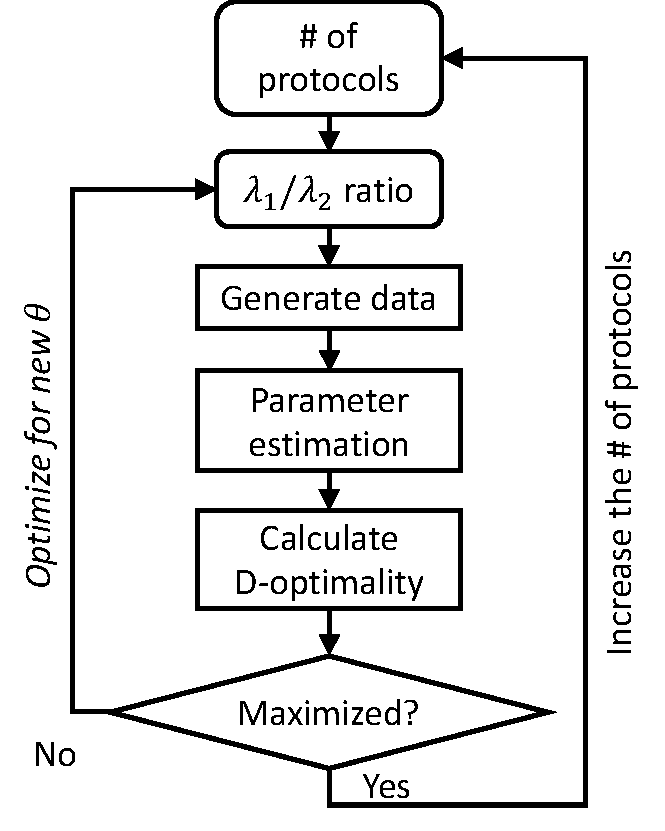
\includegraphics[width=3.25in]{Figures/optimaldesign}
\caption{Our approach for optimizing for the optimal loading paths for parameter estimation.}
\label{fig:optimaldesign}
\end{figure}
%-------------------	 end FIGURE 	-------------------%
%%%%%%%%%%%%%%%%%%%%%%%%%%%%%%%%%%%%%%%%%%%%%%%%%%%%%%%%%%%%

    
    We define loading paths based on the following conditions: 
\begin{enumerate}
\item The number of loading paths necessary
\item The number of variables needed to define a loading path and thus need to be iterated over
\item Possible application to mechanical testing of tissues.
\end{enumerate} 
Starting with planar extensions only, we chose a loading path as data points which shares the same stretch ratio, $\lambda_1/\lambda_2$, which is the same definition used for biaxial mechanical testing. This only requires one constant to be defined for each loading path and the resulting fan shape covers the largest range of deformation with the least number of data points. Next, with the total number of loading paths ranging from 1 to 6, we found 1) the total number of loading paths necessary before the benefit for adding additional loading paths is minimized and 2) the optimal ratio of the stretches for each of the individual loading path in the set (Fig. \ref{fig:optimaldesign}). Next the shear component is added. For each loading path, a parameter $\kappa_1$ for the maximum shear value reached is added to the same optimization framework (Fig. \ref{fig:optimaldesign}). For this case, we constrained the shear to be $0<\kappa_1<0.2$. Only the positive values of $\kappa_1$ is allowed due to the material symmetry. Furthermore, the optimal planar extensions loading paths are always incorporated into the dataset as a constant.



    

% %-----------------------------------------------------------
% %	Inverse parameter estimation
% %-----------------------------------------------------------
% \subsection{Inverse process for determining the parameter of high order models}

% 	The most crucial remaining question is whether the material parameters of complex downscale models can still be recovered from the response using the effective model. This is crucial for simulating time-dependent processes, which often requires recovering the material parameters of the downscale models to determine how the structural or material properties of the material parameters will change with time. For this, we compared the structural model parameter in two cases: 1) fitting the structural model to the experimental data, 2) fitting the effective model parameters to the experimental data, then fit the structural model to the response of the effective model. 
    
% %%%%%%%%%%%%%%%%%%%%%%%%%%%%%%%%%%%%%%%%%%%%%%%%%%%%%%%%%%%%
% %-------------------	begin FIGURE 	-------------------%
% \begin{figure}
% \centering
% \includegraphics[width=3.25in]{Figures/forwardinverseparameterestimation}
% \caption{Our approach testing how well the effective constitutive model can fully reproduce the mechanical response of soft tissues, and whether we can still recover the structural model parameter from the effective constitutive model.}
% \label{fig:forwardinverseparameterestimation}
% \end{figure}
% %-------------------	 end FIGURE 	-------------------%
% %%%%%%%%%%%%%%%%%%%%%%%%%%%%%%%%%%%%%%%%%%%%%%%%%%%%%%%%%%%%

%-------------------	application		-------------------%
%%%%%%%%%%%%%%%%%%%%%%%%%%%%%%%%%%%%%%%%%%%%%%%%%%%%%%%%%%%%%
%%  Model Applications										%
%%%%%%%%%%%%%%%%%%%%%%%%%%%%%%%%%%%%%%%%%%%%%%%%%%%%%%%%%%%%%

%-----------------------------------------------------------
%	Use of structural constitutive models
%-----------------------------------------------------------
\subsection{Example application for planar soft tissues}

	The example we use to test the our approach (Fig. \ref{fig:simulationframework}) is the exogenously cross-linked structural model presented in Zhang and Sacks \cite{zhang_modeling_2017}. This meso-scale structural model is computationally expensive due to integration over the collagen fiber architecture but have been shown to be able to accurately reproduce the mechanical response of a variety of soft tissues, such as mitral valve leaflets \cite{zhang_meso_2016}, ovine pulmonary artery \cite{fata_insights_2014}, myocardium \cite{avazmohammadi_novel_2017}, and exogenously cross-linked bovine pericaridium \cite{sacks_novel_2016}, and can be used to simulate the time evolving properties of bioprosthetic heart valves. To briefly summarize, this model is composed of 3 components: collagen, $\Psi_\mathrm{col}$, matrix, $\Psi_\mathrm{mat}$, and interactions, $\Psi_\mathrm{int}$. 
%==========================================================%
%-------------------	begin EQUATION 	-------------------%
\begin{equation}
\Psi 	= \Psi_\mathrm{col} + \Psi_\mathrm{mat} + \Psi_\mathrm{int} \label{eqn:structuralmodelcomponents}
\end{equation}
%-------------------	 end EQUATION 	-------------------%
%==========================================================%
The matrix term, $\Psi_\mathrm{mat}$, is a modified version of the Yeoh model that is more linear in 2nd Piola Kirchhoff stress and stretch, 
%==========================================================%
%-------------------	begin EQUATION 	-------------------%
\begin{equation}\label{eqn:matrixmodel}
\begin{aligned}
\Psi_\mathrm{mat} = &\frac{\eta_M}{2} \left[ \frac{1}{a}\left( I_1 -3\right)^{a} + \frac{r}{b} \left( I_1 -3\right)^{b} \right], \\
&\text{with } 1<a<b, ab <2, 0 \leq r.
\end{aligned}
\end{equation}
%-------------------	 end EQUATION 	-------------------%
%==========================================================%
This model contains four parameters: $\eta_M$ is the modulus parameter corresponding to the same parameter in the Neo Hookean model, $a$, $b$, and $r$ are the shape parameters, where $a$ and $b$ control the shape of the two terms, while $r$ is the weight between the two terms. In general, $a \approx 1$, $b \approx 1.87$ and $r \approx 15$ can be treated as constants. 


	The response of collagen fibers is integration over all collagen fibers architecture, their orientation and crimp. The fiber orientations is described by a beta distribution function and fiber crimp is described by a beta distribution function of the stretches needed to straighten the fibers, the slack stretch $\lambda_s$. These are referred to as the orientation distribution function (ODF), $\Gamma$, and the recruitment distribution function (RDF), $D$, respectively, with the form given in Zhang and Sacks \cite{zhang_meso_2016, zhang_modeling_2017, sacks_novel_2016}. The response of the collagen fibers is given by the sum of all fiber with respect the ODF and RDF describing the orientation and crimp of each fiber respectively,
%==========================================================%
%-------------------	begin EQUATION 	-------------------%
\begin{equation} \label{eqn:collagen}
\begin{aligned}
\Psi_\mathrm{col} =& \phi_\mathrm{col} \eta_C \int\displaylimits_\theta \Gamma(\theta) 
\int\displaylimits_1^{\lambda_\theta} D\left(\lambda_s \right) \left( \frac{\lambda_\theta}{\lambda_s} - 1\right)^2 \mathrm{d}\lambda_s \mathrm{d}\theta,
\end{aligned}
\end{equation}
%-------------------	 end equation 	-------------------%
%----------------------------------------------------------%
where $\eta_C$ is the modulus of the collagen fibers, $\lambda_\theta = \sqrt{\mathbf{n}_\theta \cdot \mathbf{C}\mathbf{n}_\theta}$ is the stretch of the ensemble of collagen fiber with the same orientation, and $\lambda_\mathrm{\theta}/\lambda_s$ is the true stretch of the collagen fibers after they are straightened \cite{zhang_meso_2016}. Similarly, the response of the interaction term is given by integration over pairs of fibers based on their orientation and crimp, which contains a quadruple integral. 
%==========================================================%
%-------------------	begin EQUATION 	-------------------%
\begin{equation}
\Psi_\mathrm{int} = \frac{\eta_I}{2} \int\displaylimits_\alpha \int\displaylimits_\beta \Gamma(\alpha) \Gamma(\beta) \int\displaylimits_1^{\lambda_\alpha} \int\displaylimits_1^{\lambda_\beta} D\left( x_\alpha \right) D\left( x_\beta \right) \left( \frac{\lambda_\alpha \lambda_\beta}{x_\alpha x_\beta} - 1\right)^2 \,\mathrm{d}x_\alpha \,\mathrm{d}x_\beta \,\mathrm{d}\alpha \,\mathrm{d}\beta.
\end{equation}
%-------------------	 end EQUATION 	-------------------%
%==========================================================%
For clarity of presentation, the slack stretches, $\lambda_s$, are replaced by $x_\alpha$ and $x_\beta$ for fiber oriented along the angle $\alpha$ and $\beta$ respectively. Only one parameter, the modulus $\eta_I$, is used to account for all interactions, with the same $\Gamma$ and $D$ already given above. 

The second Piola Kirchhoff stress of all three components of the full model (Eqn. \ref{eqn:structuralmodelcomponents}), $\mathbf{S}=2\frac{\partial\Psi}{\partial\mathbf{C}}$, is 
%==========================================================%
%-------------------	begin EQUATION 	-------------------%
\begin{equation} \label{eqn:fullcollagen}
\begin{aligned}
\mathbf{S} = & \phi_\mathrm{col} \eta_C \int\displaylimits_\theta \Gamma(\theta)\left\lbrace 
\int\displaylimits_1^{\lambda_\theta} \frac{D\left( x \right)}{x} \left( \frac{1}{x}- \frac{1}{\lambda_\theta}\right) \mathrm{d}x \right\rbrace \mathbf{n}_\theta\otimes\mathbf{n}_\theta \mathrm{d}\theta \\
+ & \phi_\mathrm{col} \eta_I \int\displaylimits_\alpha \int\displaylimits_\beta \Gamma \left(\alpha \right) \Gamma \left( \beta \right) \\
& \times \left[ \left\lbrace 
\int\displaylimits_1^{\lambda_\alpha} \int\displaylimits_1^{\lambda_\beta} 
\frac{2 \lambda_\beta D(x_\alpha) D(x_\beta)}{x_\alpha x_\beta} 
\left( \frac{\lambda_\alpha}{x_\alpha} \frac{\lambda_\beta}{x_\beta} - 1\right) \mathrm{d}x_\alpha \, \mathrm{d}x_\beta 
+\int\displaylimits_1^{\lambda_\beta} D(x_\beta) \left( \frac{\lambda_\beta}{x_\beta} -1  \right)^2 \mathrm{d}x_\beta \right\rbrace \right.  \frac{\mathbf{n}_\alpha \otimes \mathbf{n}_\alpha}{\lambda_\alpha}  \\
& + \left. \left\lbrace
\int\displaylimits_1^{\lambda_\alpha} \int\displaylimits_1^{\lambda_\beta} 
\frac{2 \lambda_\alpha D(x_\alpha) D(x_\beta)}{x_\alpha x_\beta} 
\left( \frac{\lambda_\alpha}{x_\alpha} \frac{\lambda_\beta}{x_\beta} - 1\right) \mathrm{d}x_\alpha \, \mathrm{d}x_\beta 
+ \int\displaylimits_1^{\lambda_\alpha} D(x_\alpha) \left( \frac{\lambda_\alpha}{x_\alpha} -1  \right)^2 \mathrm{d}x_\alpha \right\rbrace \frac{\mathbf{n}_\beta \otimes \mathbf{n}_\beta}{\lambda_\beta}  \right] \mathrm{d}\alpha \, \mathrm{d}\beta\\
+ & \phi_\mathrm{mat} \eta_M \left[\left(\left( I_1 - 3\right)^{a - 1} + r \left( I_1 - 3\right)^{b - 1}\right) \left( \mathbf{I} - C_{33}\mathbf{C}^{-1}\right)  \right],\\
\end{aligned}
\end{equation}
%-------------------	 end EQUATION 	-------------------%
%==========================================================%
where $\phi_\mathrm{col}$ and $\phi_\mathrm{mat}$ are the mass fraction of collagen and matrix respectively. 
    
	Although very accurate and predictive, this model is not only computationally expensive, numerical integration results in a significant decrease in numerical precision when the number of quadrature point is insufficient. This can create a number of issues for convergence during parameter optimization. Thus, the implementation of this model is complicated by a constant balance between computational cost and numerical robustness during optimization. Using $\Psi_{eff}$ (Eqn. \ref{eqn:finalexponentialmodelformscaled}) is a solution to these issues. Furthermore, some modifications can be made to reduce the form of the model if necessary based on how well each term captures the behavior of the respective material (see Appendix \ref{sec:specificform}).
    
    
    



	











%---------------	parameter estimation	---------------%
%-----------------------------------------------------------
%	Parameter estimation
%-----------------------------------------------------------
\subsection{Parameter estimation}

	The objective function form we use is 
%==========================================================%
%-------------------	begin EQUATION 	-------------------%
\begin{subequations}\label{eqn:objectivefunction}
\begin{gather}
S_m = \dpd{\Psi}{E_m} = \mathbf{m}_0\cdot\mathbf{S}\mathbf{m}_0,
	\quad S_n = \dpd{\Psi}{E_n} = \mathbf{n}_0\cdot\mathbf{S}\mathbf{n}_0,
    \quad S_\phi = \dpd{\Psi}{E_\phi} = 2\mathbf{m}_0\cdot\mathbf{S}\mathbf{n}_0 \label{eqn:responsefunctions}\\
\mathcal{F} = \sum_i^n \left(S_m(\hat{E}_M^i, \hat{E}_S^i, \hat{E}_\phi^i) - \hat{S}_M^i \right)^2 + \left(S_n(\hat{E}_M^i, \hat{E}_S^i, \hat{E}_\phi^i) - \hat{S}_S^i \right)^2 + \left(S_\phi(\hat{E}_M^i, \hat{E}_S^i, \hat{E}_\phi^i) - \hat{S}_\phi^i \right)^2
\end{gather}
\end{subequations}
%-------------------	 end EQUATION 	-------------------%
%==========================================================%
This removes rigid body rotation and puts the stresses along the material axes, thus casts the stresses are the response functions directly and minimizes covariance between the parameters during optimization. The choice L2-norm, sum of the difference of the squares of the stresses, is the most popular. Other possible options include the log of the L2-norm, the log-norm presented by Aggarwal \cite{aggarwal_improved_2017}, and L2-norm of the strain energy, and the other stress measures.

	For optimal speed when using $\Psi_{eff}$ (Eqn. \ref{eqn:finalexponentialmodelformscaled}) to homogenize micro-models, gradient methods are ideal, which are the fastest. Because we require some non-linear constraint to enforce convexity, we utilized the interior point algorithm provided by the IPOPT library \cite{waechter_implementation_2005}. The initial guess is easily derived for the model scaling method, with the parameter $c_0$ being the maximum strain energy in the available data. The exponent parameters $b_i$ are generally very consistent in value, with the quadratic parameters being $b_1 \approx 10$, $b_2 \approx 10$, and $b_4 \approx -10$, the quartic parameters being $b_5 \approx 2000$, $b_6 \approx 500$, $b_9 \approx 200$, $b_{10} \approx 200$, $b_{11} \approx 200$, $b_{12} \approx 200$. We find this setup to work extremely well, and no further modification being necessary. 




\subsection{Reproducing the response of soft tissues using the effective constitutive model and optimal loading paths}\label{sec:reproducefung}

	For our approach of using the effective constitutive models to facilitate numerical simulation (Fig. \ref{fig:simulationframework}), we need to overcome the limitation of common phenomenological approaches on predicting the mechanical response of micro-models outside of the data set used for parameter estimation \cite{sun_biaxial_2003}. For this, we will first reproduced the results of Sun \textit{et al.} \cite{sun_biaxial_2003} using the generalized Fung model, then repeat the process using $\Psi_{eff}$ (Eqn. \ref{eqn:finalexponentialmodelformscaled}) with optimal loading paths. We will focus on glutaraldehyde cross-linked bovine pericardium for the soft tissue. Bovine pericardium is the most common material used to fabricate bioprosthetic heart valves. It is extremely dense in collagenous fibers, having broad fiber splays with approximately $30\deg$ in standard deviation. The resulting mechanical behavior have strong coupling between the axial stretches. Thus, the mechanical response of some bovine pericardium specimens are fitted to the structural model (Eqn. \ref{eqn:fullcollagen}). The structural model is then used to generate stress strain data along loading paths with stress ratios ($S_{11}/S_{22}$) of $0.1:1$, $0.5:1$, $0.75:1$, $1:1$, $1:0.75$, $1:0.5$, and $1:0.1$. Following Sun \textit{et al.} \cite{sun_biaxial_2003}, the generalized Fung model (Eqn. \ref{eqn:generalizedfungmodela}) was fitted to the five loading paths in the physiologic range ($0.5:1$, $0.75:1$, $1:1$, $1:0.75$, $1:0.5$), then the remain two loading paths were predicted and compared to the data. The reverse scenario was done, where the generalized Fung model was fitted to the non-physiologic loading paths ($0.1:1$ and $1:0.1$) while the remaining five loading paths were predicted. Following the same step, $\Psi_{eff}$ was fitted to the three optimal loading paths ($0.1:1$, $1:1$, and $1:0.1$) while the remaining loading paths were predicted. 
    
    We also considered some alternative loading paths. In the original paper by Fung et al. on the constitutive modeling of arteries \cite{fung_pseudoelasticity_1979}, they discussed the use of 'physiologic protocols' as the optimal data set for parameter estimation. These 'physiologic protocols' are loading paths that covers a range larger than some lower bounds for $E_{11}$ and $E_{22}$. Conceptually, this is meant to correspond to the range after accounting for the pre-strain between the zero stress configuration and the \textit{in vivo} unloaded (not stress free) configuration. For clarity, to distinguish between this and the physiologic range (the range where the physiologic loading path is likely to reside) in Sun \textit{et al.}, we will refer to this as the post-pre-strain range. We reproduced the post-pre-strain protocols in figure 5 of Fung \textit{et al.} \cite{fung_pseudoelasticity_1979}, and compared the results to using the optimal loading paths. 
    
	For other soft tissues and alternative model forms, see Appendix \ref{sec:otherresults}







%-------------------	simulation		-------------------%
\subsection{Numerical simulations}

	A exhaustive numerical study using $\Psi_{eff}$ (Eqn. \ref{eqn:finalexponentialmodelformscaled}) is beyond the scope of this work. However, we hereby present an example implementation of the framework we proposed (Fig. \ref{fig:simulationframework}) using the structural model (Eqn. \ref{eqn:fullcollagen}) and $\Psi_{eff}$ (Eqn. \ref{eqn:finalexponentialmodelformscaled}) to facilitating numerical simulation of intact bioprothetic heart valves. The leaflet material consider are bovine pericardium (most commonly used for bioprothetic heart valve leaflets), porcine aortic valve (highly anisotropy response), and bovine pericardium with an uniform fiber ODF (isotropic). We replicated the response of these tissues using the structural model based on their microstructure. We then fit $\Psi_{eff}$ to the structural model by sampling along optimal loading paths. Next, we evaluated the computational cost and numerical robustness of $\Psi_{eff}$ and its ability to handle a wide range of material properties and the complex \textit{in vivo} deformations in numerical simulations.
    
    
    For numerical simulation, we utilized the custom finite element simulation software developed by Hsu \textit{et al.} \cite{hsu_dynamic_2015, kamensky_immersogeometric_2015, kiendl_isogeometric_2015}. Briefly, the finite element code was developed for isogeometric fluid solid dynamics simulation of heart valves, focusing mostly on the tri-leaflet atrioventricular valves. The tri-leaflet geometry is based on the commonly used Edwards Pericardial Heart Valve with Kirchhoff-Love shells for the leaflets \cite{kiendl_isogeometric_2015}. We utilized the quasi-static portion of the code for simulations of leaflet deformations at physiologic pressure (80 mmHg). The implementation of $\Psi_{eff}$ was validated using biaxial mechanical testing simulations (Appendix \ref{sec:biaxialsimulation}, Fig. \ref{fig:biaxvalidation}). A total was 484 B\'ezier elements was used for each leaflets, and the leaflet thickness was assumed to be uniform and 0.386mm thick \cite{hsu_dynamic_2015}. For simplicity and consistency, the collagen fiber direction was assume to be uniform along the circumferential direction of each leaflet. No root, atrial chamber or the surrounding artery was used. The bioprothetic heart valve stent was made rigid and undeformable, serving a stationary reference for the leaflets. 
%-----------------------------------------------------------
%	Simulations												
%-----------------------------------------------------------

 



%-----------------------------------------------------------
%	Forward and backwards simulations
%-----------------------------------------------------------

% \subsection{Simulating the structural model response}
% \subsubsection{Forward and backwards simulation}
% \subsubsection{Validation}


%-----------------------------------------------------------
%	Planar Biaxial Simulation
%-----------------------------------------------------------


%-----------------------------------------------------------
%	Tri-leaflet valve simulations
%-----------------------------------------------------------













%-----------------------------------------------------------
%	Results
%-----------------------------------------------------------

%%%%%%%%%%%%%%%%%%%%%%%%%%%%%%%%%%%%%%%%%%%%%%%%%%%%%%%%%%%%%
%%	Results													%
%%%%%%%%%%%%%%%%%%%%%%%%%%%%%%%%%%%%%%%%%%%%%%%%%%%%%%%%%%%%%

\section{Results}

%-----------------------------------------------------------
%	Model fit
%-----------------------------------------------------------
\subsection{Model fit and parameter estimation}



	Using $\Psi_{eff}$ (Eqn. \ref{eqn:finalexponentialmodelformscaled}) significantly improves the fit to the responses of the structural model (Eqn. \ref{eqn:fullcollagen}) with an average $R^2$ of 0.958 (n = 6). Specifically, the improvement is mainly in fitting the non-physiologic range, defined as the range away from the equi-biaxial strain region, specifically uniaxial strain or pure shear (Fig. \ref{fig:modelfit}). The time taken for parameter estimation (5-10 seconds) is also significantly lower in comparison to meso-scale structural approaches, such for the mitral valve \cite{zhang_meso_2016} (10-40 minutes) and exogenously crosslinked tissues \cite{zhang_modeling_2017}(30 min - 4 hours).
    
%%%%%%%%%%%%%%%%%%%%%%%%%%%%%%%%%%%%%%%%%%%%%%%%%%%%%%%%%%%%
%-------------------	begin FIGURE 	-------------------%
\begin{figure}
\centering
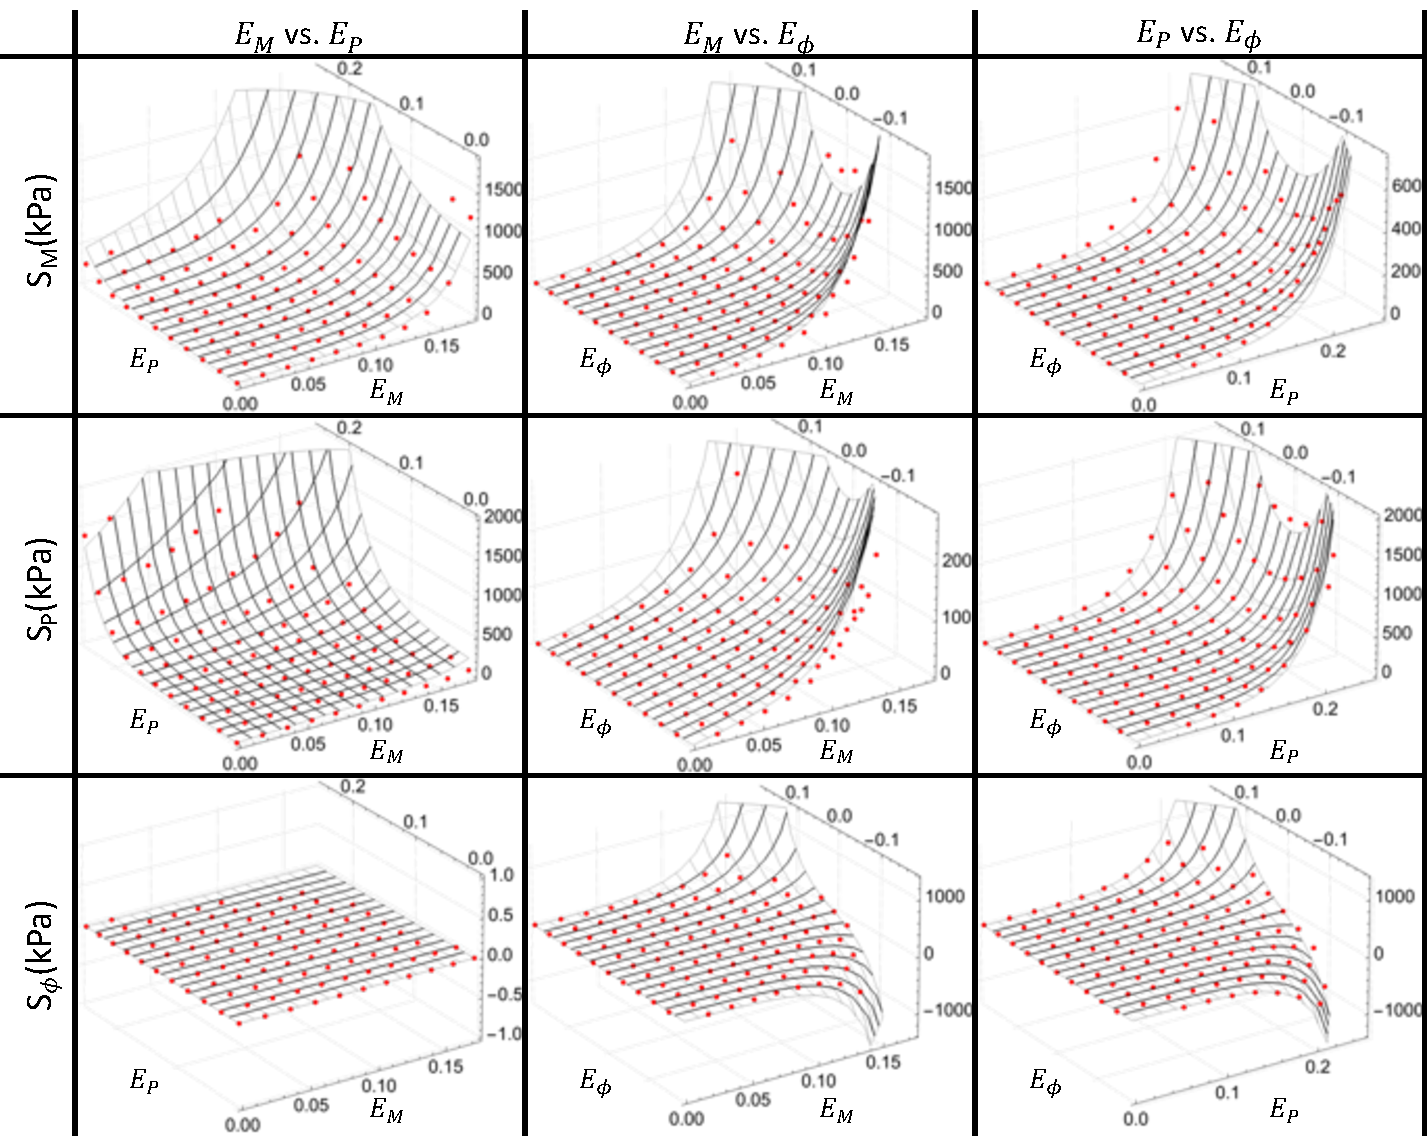
\includegraphics[width=6.5in]{Figures/modelfit}
\caption{Parameter estimation results showing that $\Psi_{eff}$ is able to match response function (Eqn. \ref{eqn:responsefunctions}) (Top) $S_m = \partial\Psi/\dif E_m$, (Middle) $S_n = \partial\Psi/\dif E_n$, and (Bottom) $S_\phi = \partial\Psi/\dif E_\phi$ for each pair of Green Lagrange strain components.}
\label{fig:modelfit}
\end{figure} 
%-------------------	 end FIGURE 	-------------------%
%%%%%%%%%%%%%%%%%%%%%%%%%%%%%%%%%%%%%%%%%%%%%%%%%%%%%%%%%%%%
    
%     Furthermore, we found that fitting the effective model to existing data sufficiently preserves the mechanical response of glutaraldehyde pericardium such that we were able to obtain similar structural model parameters in comparison to fitting to the structural model directly. There are some minor differences, especially in the modulus, but that is impart due to the fact that the experimental data is somewhat lacking, particularly in terms of examining the response of the material to shearing, but this is still enough for us to obtain reasonably accurate structural model parameters. The accuracy can be further improved if we import the microstructural of the material, the ODF and RDF, directly.  

% %----------------------------------------------------------%
% %-------------------	begin TABLE 	-------------------%
% \begin{table}
% \caption{Comparison between structural model parameters when fitting to the experimental data directly vs. to the effective constitutive model fitted to the experimental data. UB is the abbreviation for upper-bound.}
% \begin{center}
% \label{tb:inverseparameterestimation}
% \begin{tabular}{|l|p{40pt}|p{45pt} p{25pt} p{25pt} p{25pt} p{25pt} p{25pt}|p{60pt}|}
% \hline

%  	& \centering Matrix \mbox modulus (kPa)	
%     & \centering Collagen \mbox{modulus} (kPa)	
%     & \centering ODF mean $(\deg)$	
%     & \centering ODF stdev	$(\deg)$ 
%     & {\centering $D(\lambda_s)$ mean}
%     & \centering $D(\lambda_s)$ stdev	
%     & {\centering $D(\lambda_s)$ UB}
%     & {\centering Interactions modulus (kPa)}\\
% \hline
% FSM to data	& 102.8	& 302	& 0	& 32.7	& 1.187	& 0.022	& 1.213	& 1785.7	\\
% \hline
% FSM to EMM	& 97.1	& 288	& 0	& 34.1	& 1.192	& 0.023 & 1.221	& 2085.3	\\
% \hline
% \end{tabular}
% \end{center}
% \end{table}
% %-------------------	 end TABLE 		-------------------%
% %----------------------------------------------------------%


%-----------------------------------------------------------
%	Parameter estimation convergence
%-----------------------------------------------------------
\subsection{Convergence}

	In addition, we found that the model scaling method is very effective. Parameters converges in approximately 40-60 iterations regardless of starting point, where are the algorithm can require 40-120 iterations without using scaling. This is of course due to the fact that the algorithm can be trapped within the valley region where the gradient is small, reducing the step size during search. Of course, with sufficiently good initial guess, both methods are essentially equivalent.



%-----------------------------------------------------------
%	Optimal experimental design
%-----------------------------------------------------------
\subsection{Optimal \textit{in silico} loading paths}

	Based on our results, the optimal loading paths for parameter estimation is rather intuitive. For a single loading path, this is the equi-biaxial stress loading path. D-optimality is several hundred times higher for the equi-biaxial stress loading path in comparison to all other loading paths, i.e. the D-optimality for other loading paths are nearly zero. Even so the D-optimality is still on the order of $10^{-17}$, implying that a single loading path is not sufficient to determine the model parameters of highly non-linear hyperelastic tissues. The type of stress is not explicitly listed, rather this depends on the choice of objective function, i.e. if the parameter estimation is done using the difference in second Piola Kirchhoff stress then the choice of the loading path should be equi-biaxial in second Piola Kirchhoff stress. 
    
    
%%%%%%%%%%%%%%%%%%%%%%%%%%%%%%%%%%%%%%%%%%%%%%%%%%%%%%%%%%%%
%-------------------	begin FIGURE 	-------------------%
\begin{figure}[hbtp]
\centering
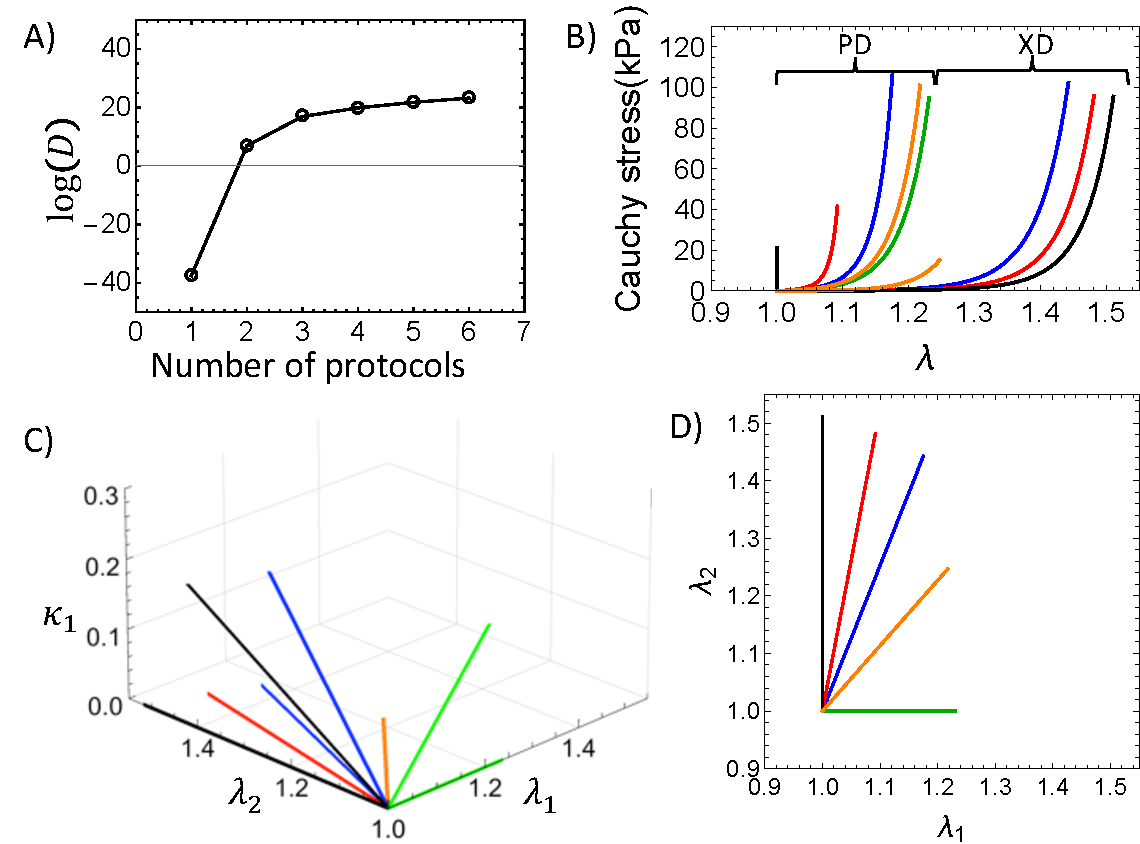
\includegraphics[width=5.5in]{Figures/doptimality}
\caption{A) The best D-optimality value for a given number of loading paths used to generate the data, which stops increasing significantly after three. B) The stress-strain curve of the optimal set of five loading paths with no shear. C) The full set of optimal loading paths including the shear component are shown. The same colored loading paths are built upon the corresponding D) planar stretch loading paths by adding a shear component. }
\label{fig:doptimality}
\end{figure} 
%-------------------	 end FIGURE 	-------------------%
%%%%%%%%%%%%%%%%%%%%%%%%%%%%%%%%%%%%%%%%%%%%%%%%%%%%%%%%%%%%

    
    The value of D-optimality significantly improved with the addition of a second loading path, increasing from $5.2 \times 10^{-17}$ to $9.7 \times 10^2$, nearly 20 orders in magnitude. Using three loading paths leads to another significant increase to $2.2 \times 10^7$, 5 orders of magnitude. Further additional loading paths only improve the D-optimality by 1 order of magnitude, where the D-optimality is $4.2 \times 10^8$, $2.8 \times 10^9$ and $1.2 \times 10^{10}$ for four, five and sixth loading paths respectively. It can be said that three is the minimal number of loading paths necessary for parameter estimation. Indeed, for dense collagenous soft tissues this appears to be true. In practice, it's better to add a few additional loading paths as a precaution. For this reason, using five loading paths is more preferred (Fig. \ref{fig:doptimality}D). The reason why four loading paths is not chosen is because the specific loading paths are not consistent and maybe even model dependent if it is even (see Appendix \ref{sec:optimalpaths}, Fig. \ref{fig:evenpaths}). For odd number of loading paths, these are the equibiaxial stress, the boundaries of the range of interest, and the average ratios in between (see Appendix \ref{sec:optimalpaths}, Fig. \ref{fig:oddpaths}). With the addition of shear, we found this to be the minimal three loading paths adding to it a shear component up to the maximum value (Fig. \ref{fig:doptimality}C). Further addition does not change the D-optimality by any significant quantity. More detailed results are presented in Appendix \ref{sec:optimalpaths}.
    
    
  
% phy1 norm = 1.35315
% phy3 norm = 19834.0


   

%-----------------------------------------------------------
%	Vs Fung
%-----------------------------------------------------------
\subsection{Reproducing soft tissue response}

	For the Sun \textit{et al.} \cite{sun_biaxial_2003} study, the generalized Fung model (Eqn. \ref{eqn:generalizedfungmodela}) fitted the five loading paths in the physiologic range very well (Fig. \ref{fig:fungphyfit}), but predicted the remaining unfitted loading paths poorly (Fig. \ref{fig:fungphypred}). Similarly, when the non-physiologic loading paths are fit ((Fig. \ref{fig:fungphyfit})), the remaining protocols are still predicted poorly. However, we do note here that the generalized Fung model cannot fit the non-physiologic protocols very well. This is as expected since the generalized Fung model can only approximate the response of soft tissues in a limited range (Section \ref{sec:possibleforms}). 

%%%%%%%%%%%%%%%%%%%%%%%%%%%%%%%%%%%%%%%%%%%%%%%%%%%%%%%%%%%%
%-------------------	begin FIGURE 	-------------------%
\begin{figure}[hptb]
\centering
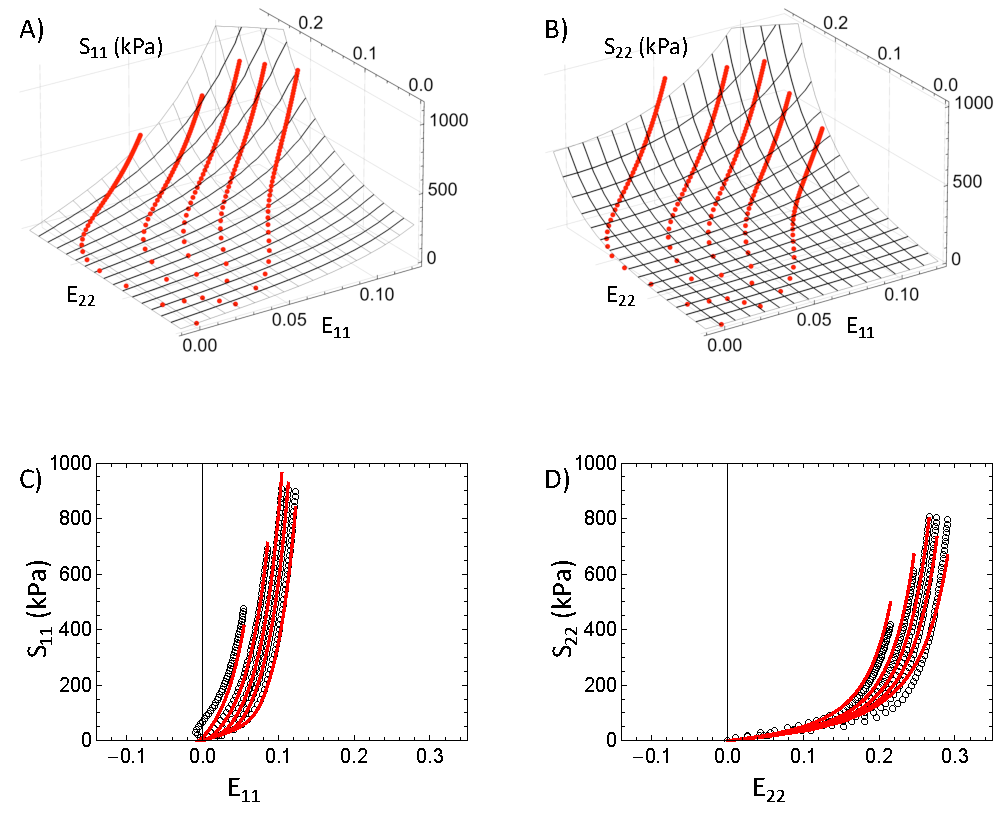
\includegraphics[width=6.5in]{Figures/fungphyfit}
\caption{Reproducing the results of Sun \textit{et al.} \cite{sun_biaxial_2003} showing that the generalized Fung model is able to fit the loading paths in the physiologic range very well. A) The $S_{11}$ surface. B) The $S_{22}$ surface. C) Best fit of the $S_{11}$ component of the loading paths. D) Best fit of the $S_{22}$ component of the loading paths.}
\label{fig:fungphyfit}
\end{figure} 
%-------------------	 end FIGURE 	-------------------%
%%%%%%%%%%%%%%%%%%%%%%%%%%%%%%%%%%%%%%%%%%%%%%%%%%%%%%%%%%%%

%%%%%%%%%%%%%%%%%%%%%%%%%%%%%%%%%%%%%%%%%%%%%%%%%%%%%%%%%%%%
%-------------------	begin FIGURE 	-------------------%
\begin{figure}[hptb]
\centering
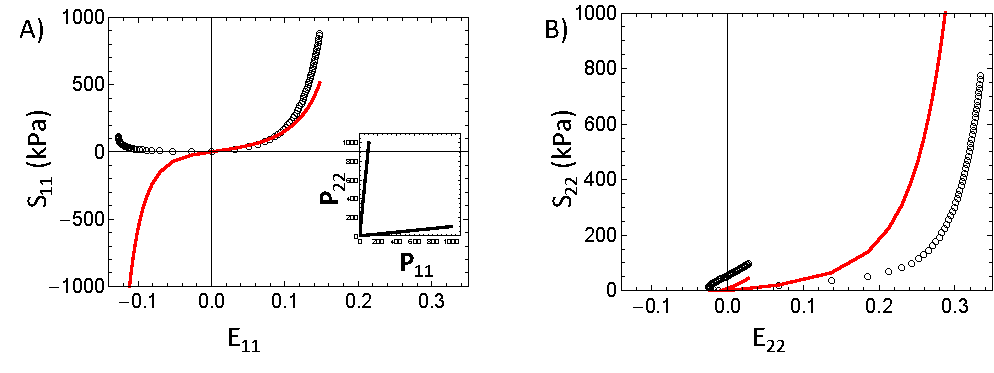
\includegraphics[width=6.5in]{Figures/fungphypred}
\caption{Reproducing the results of Sun \textit{et al.} \cite{sun_biaxial_2003} showing the A) $S_{11}$ component and B) $S_{22}$ component of the remaining unfitted loading paths are predicted poorly from fit (Fig. \ref{fig:fungphyfit}). The inset in A shows the corresponding loading paths.}
\label{fig:fungphypred}
\end{figure} 
%-------------------	 end FIGURE 	-------------------%
%%%%%%%%%%%%%%%%%%%%%%%%%%%%%%%%%%%%%%%%%%%%%%%%%%%%%%%%%%%%


%%%%%%%%%%%%%%%%%%%%%%%%%%%%%%%%%%%%%%%%%%%%%%%%%%%%%%%%%%%%
%-------------------	begin FIGURE 	-------------------%
\begin{figure}[hptb]
\centering
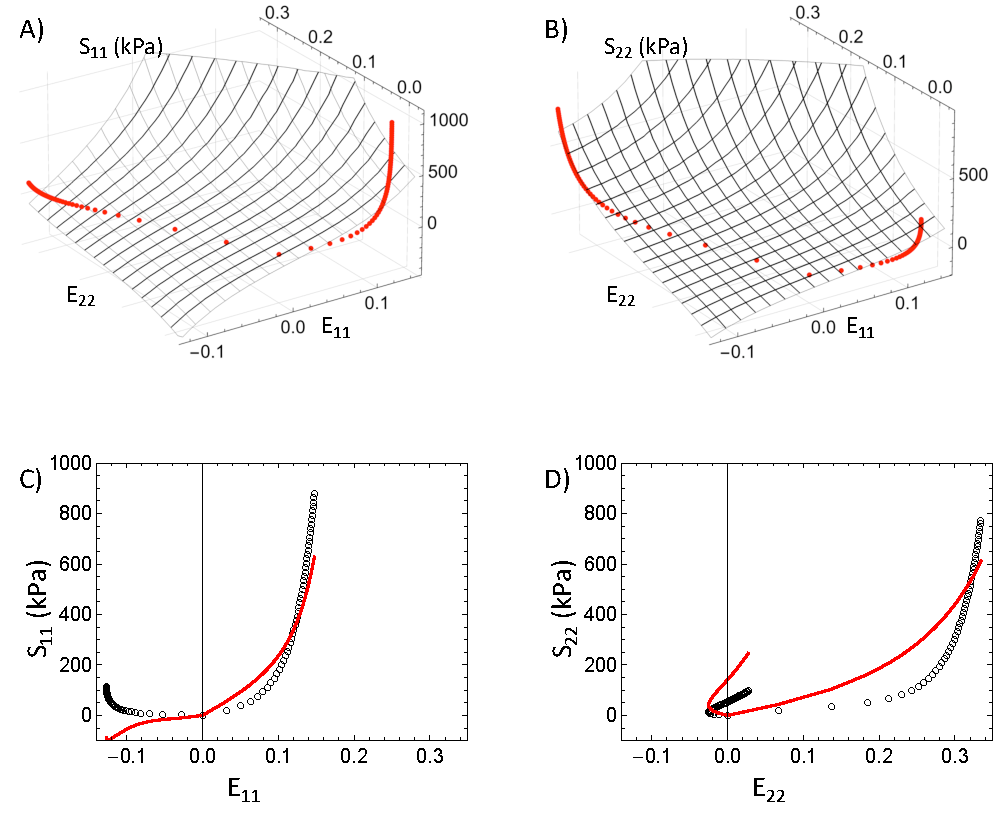
\includegraphics[width=6.5in]{Figures/fungoutfit}
\caption{Reproducing the results of Sun \textit{et al.} \cite{sun_biaxial_2003} showing the best fit of the generalized Fung model to the loading paths in the non-physiologic range is poor. A) The $S_{11}$ surface. B) The $S_{22}$ surface. C) Best fit of the $S_{11}$ component of the loading paths. D) Best fit of the $S_{22}$ component of the loading paths.}
\label{fig:fungoutfit}
\end{figure} 
%-------------------	 end FIGURE 	-------------------%
%%%%%%%%%%%%%%%%%%%%%%%%%%%%%%%%%%%%%%%%%%%%%%%%%%%%%%%%%%%%

%%%%%%%%%%%%%%%%%%%%%%%%%%%%%%%%%%%%%%%%%%%%%%%%%%%%%%%%%%%%
%-------------------	begin FIGURE 	-------------------%
\begin{figure}[hptb]
\centering
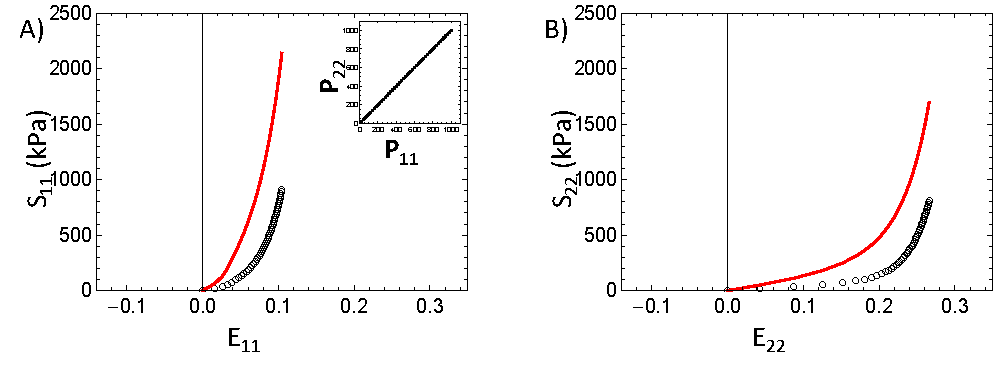
\includegraphics[width=6.5in]{Figures/fungoutpred}
\caption{Reproducing the results of Sun \textit{et al.} \cite{sun_biaxial_2003} showing the A) $S_{11}$ component and B) $S_{22}$ component of the equi-biaxial stress loading path are predicted poorly from fit (Fig. \ref{fig:fungoutfit}). The inset in A shows the corresponding loading paths.}
\label{fig:fungoutpred}
\end{figure} 
%-------------------	 end FIGURE 	-------------------%
%%%%%%%%%%%%%%%%%%%%%%%%%%%%%%%%%%%%%%%%%%%%%%%%%%%%%%%%%%%%
    

    
    

    
    
    
% %%%%%%%%%%%%%%%%%%%%%%%%%%%%%%%%%%%%%%%%%%%%%%%%%%%%%%%%%%%%
% %-------------------	begin FIGURE 	-------------------%
% \begin{figure}[!hbtp]
% \centering
% \includegraphics[width=4.5in]{Figures/sunreproduce}
% \caption{Reproducing the fit of the generalized Fung model to A) the loading paths in the physiologic range (range most likely to contain the physiologic loading path) and B) the non-physiologic loading paths in Sun \textit{et al.} \cite{sun_biaxial_2003}}
% \label{fig:sunreproduce}
% \end{figure} 
% %-------------------	 end FIGURE 	-------------------%
% %%%%%%%%%%%%%%%%%%%%%%%%%%%%%%%%%%%%%%%%%%%%%%%%%%%%%%%%%%%%

% %%%%%%%%%%%%%%%%%%%%%%%%%%%%%%%%%%%%%%%%%%%%%%%%%%%%%%%%%%%%
% %-------------------	begin FIGURE 	-------------------%
% \begin{figure}[!hbtp]
% \centering
% \includegraphics[width=6.5in]{Figures/sunstresses}
% \caption{Reproducing the resulting stress strain behavior of 1) the fitted response and 2) the prediction of the remaining loading paths of the generalized Fung model to A) the loading paths in the physiologic range and B) the non-physiologic loading paths in Sun \textit{et al.} \cite{sun_biaxial_2003}}
% \label{fig:sunstresses}
% \end{figure} 
% %-------------------	 end FIGURE 	-------------------%
% %%%%%%%%%%%%%%%%%%%%%%%%%%%%%%%%%%%%%%%%%%%%%%%%%%%%%%%%%%%%

% %%%%%%%%%%%%%%%%%%%%%%%%%%%%%%%%%%%%%%%%%%%%%%%%%%%%%%%%%%%%
% %-------------------	begin FIGURE 	-------------------%
% \begin{figure}[!hbtp]
% \centering
% \includegraphics[width=4.5in]{Figures/effectivereproduce}
% \caption{The response of fitting $\Psi_{eff}$ to A) minimal 3 optimal loading paths and B) the post pre-strain region define in Fung \textit{et al.} \cite{fung_pseudoelasticity_1979}}
% \label{fig:effectivereproduce}
% \end{figure} 
% %-------------------	 end FIGURE 	-------------------%
% %%%%%%%%%%%%%%%%%%%%%%%%%%%%%%%%%%%%%%%%%%%%%%%%%%%%%%%%%%%%
% %%%%%%%%%%%%%%%%%%%%%%%%%%%%%%%%%%%%%%%%%%%%%%%%%%%%%%%%%%%%
% %-------------------	begin FIGURE 	-------------------%
% \begin{figure}[!hbtp]
% \centering
% \includegraphics[width=6.5in]{Figures/effectivestresses}
% \caption{The stress strain behavior of 1) the fitted response and 2) the prediction of the other loading paths using $\Psi_{eff}$ to A) optimal loading paths and B) the physiologic or post pre-strain range only.}
% \label{fig:effectivestresses}
% \end{figure} 
% %-------------------	 end FIGURE 	-------------------%
% %%%%%%%%%%%%%%%%%%%%%%%%%%%%%%%%%%%%%%%%%%%%%%%%%%%%%%%%%%%%

    
	Although the quality of fit is improved with $\Psi_{eff}$ (Eqn. \ref{eqn:finalexponentialmodelformscaled}) (Fig. \ref{fig:effphyfit}), using non-optimal loading paths, such as based on Fung \textit{et al.}'s post-pre-strain protocols \cite{fung_pseudoelasticity_1979}, lead to poor predictions for other loading paths (Fig. \ref{fig:effphypred}). Although not obvious at first, $\Psi_{eff}$ severe underestimates the response of the material in the low stress region. The D-optimality with two protocols in this post-pre-strain range is only $1.35$, which improves to $1.98\times 10^4$ with six protocols. This pales in comparison to in comparison to with $9.7 \times 10^2$ for the two optimal protocols and $2.2 \times 10^7$ with three optimal protocols. When both $\Psi_{eff}$ and three optimal loading paths are utilized, we find that the loading paths are both fitted (Fig. \ref{fig:effoptfit}) and predicted very well (Fig. \ref{fig:effoptpred}). We also testing other non-optimal loading paths with minor modifications to the form of $\Psi_{eff}$ (Appendix \ref{sec:otherresults}). To briefly summarize, without an optimal set of loading paths, $\Psi_{eff}$ is not able to fully predict out side of the fitted range. When this happens, the form of $\Psi_{eff}$ can have unpredictable impact on the predicted response, even though the quality of fit are very similar. 


%%%%%%%%%%%%%%%%%%%%%%%%%%%%%%%%%%%%%%%%%%%%%%%%%%%%%%%%%%%%
%-------------------	begin FIGURE 	-------------------%
\begin{figure}[hptb]
\centering
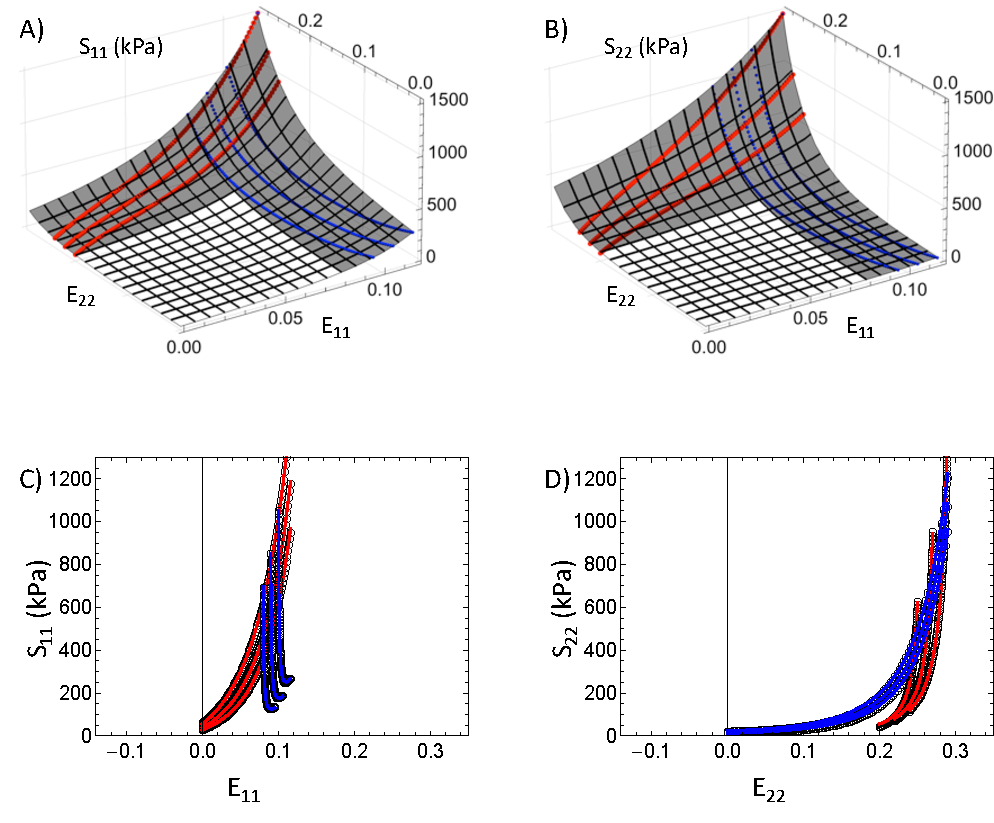
\includegraphics[width=6.5in]{Figures/effphyfit}
\caption{The fit of $\Psi_{eff}$ to the post-pre-strain loading paths is very good. A) The $S_{11}$ surface. B) The $S_{22}$ surface. C) Best fit of the $S_{11}$ component of the loading paths. D) Best fit of the $S_{22}$ component of the loading paths.}
\label{fig:effphyfit}
\end{figure} 
%-------------------	 end FIGURE 	-------------------%
%%%%%%%%%%%%%%%%%%%%%%%%%%%%%%%%%%%%%%%%%%%%%%%%%%%%%%%%%%%%

%%%%%%%%%%%%%%%%%%%%%%%%%%%%%%%%%%%%%%%%%%%%%%%%%%%%%%%%%%%%
%-------------------	begin FIGURE 	-------------------%
\begin{figure}[hptb]
\centering
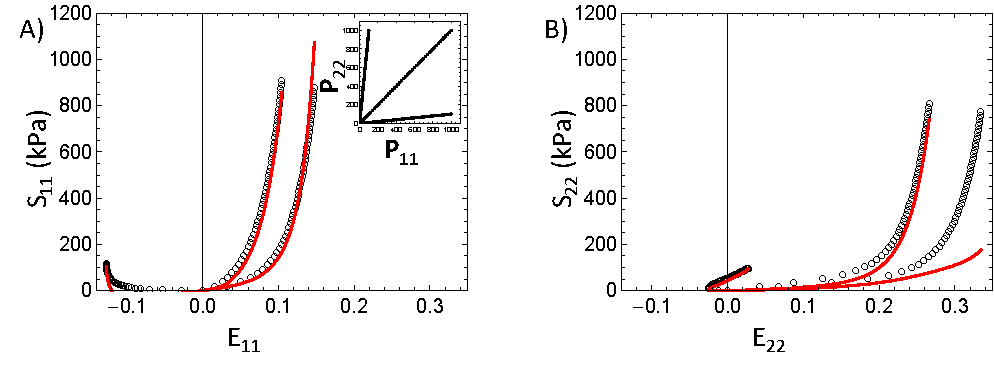
\includegraphics[width=6.5in]{Figures/effphypred}
\caption{$\Psi_{eff}$ predicts the A) $S_{11}$ component and B) $S_{22}$ component of the unfitted loading paths very poorly even though the fit to the post-pre-strain range is very good (Fig. \ref{fig:effphyfit}). The inset in A shows the corresponding loading paths.}
\label{fig:effphypred}
\end{figure} 
%-------------------	 end FIGURE 	-------------------%
%%%%%%%%%%%%%%%%%%%%%%%%%%%%%%%%%%%%%%%%%%%%%%%%%%%%%%%%%%%%


	

%%%%%%%%%%%%%%%%%%%%%%%%%%%%%%%%%%%%%%%%%%%%%%%%%%%%%%%%%%%%
%-------------------	begin FIGURE 	-------------------%
\begin{figure}[hptb]
\centering
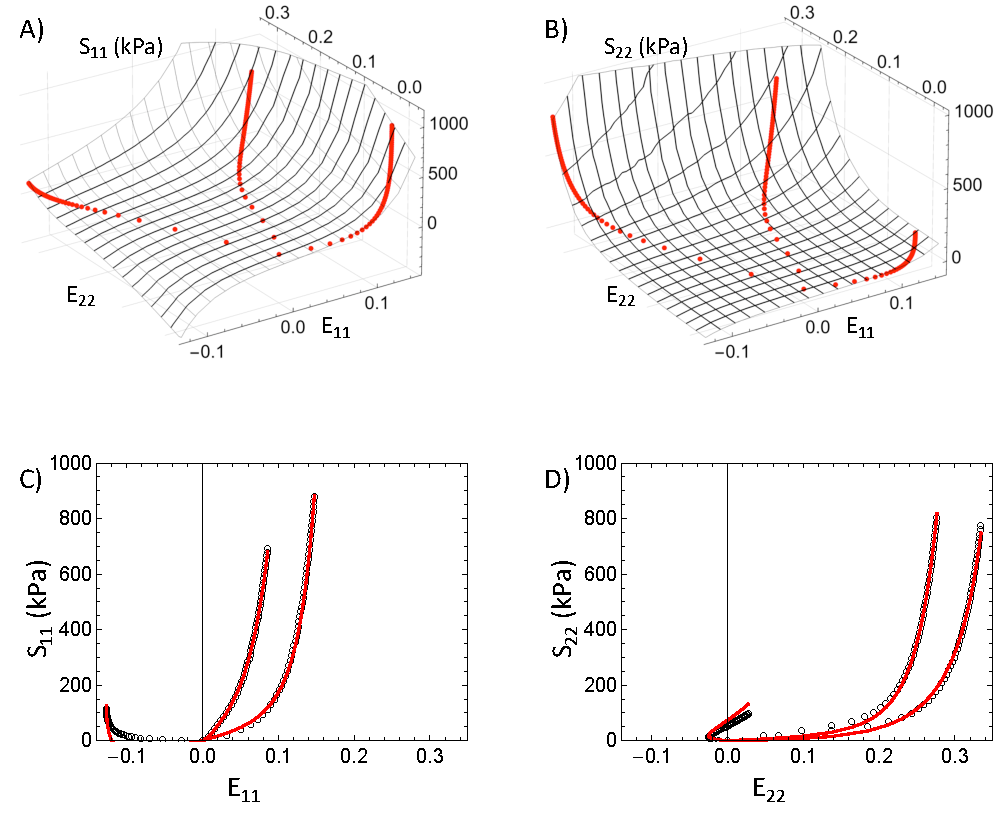
\includegraphics[width=6.5in]{Figures/effoptfit}
\caption{$\Psi_{eff}$ fit optimal loading paths very well. A) The $S_{11}$ surface. B) The $S_{22}$ surface. C) Best fit of the $S_{11}$ component of the loading paths. D) Best fit of the $S_{22}$ component of the loading paths.}
\label{fig:effoptfit}
\end{figure} 
%-------------------	 end FIGURE 	-------------------%
%%%%%%%%%%%%%%%%%%%%%%%%%%%%%%%%%%%%%%%%%%%%%%%%%%%%%%%%%%%%

%%%%%%%%%%%%%%%%%%%%%%%%%%%%%%%%%%%%%%%%%%%%%%%%%%%%%%%%%%%%
%-------------------	begin FIGURE 	-------------------%
\begin{figure}[hptb]
\centering
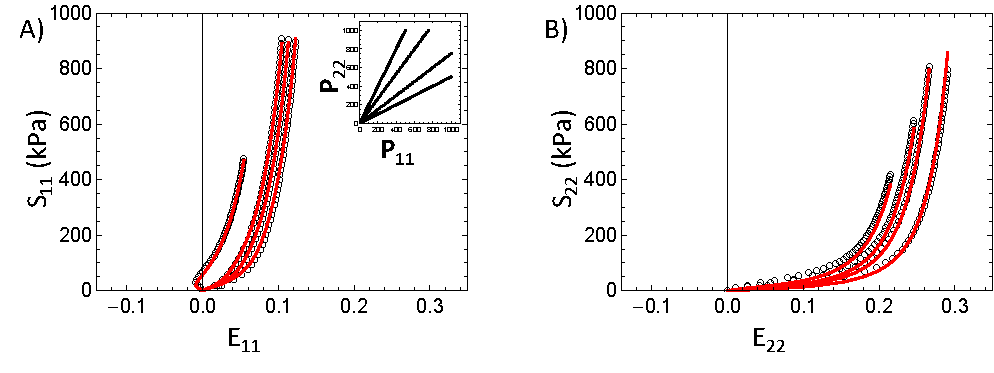
\includegraphics[width=6.5in]{Figures/effoptpred}
\caption{Combining $\Psi_{eff}$ with optimal loading paths to predicts the A) $S_{11}$ component and B) $S_{22}$ component of the remaining unfitted loading paths very well from fit (Fig. \ref{fig:effoptfit}). The inset in B shows the corresponding loading predicted paths.}
\label{fig:effoptpred}
\end{figure} 
%-------------------	 end FIGURE 	-------------------%
%%%%%%%%%%%%%%%%%%%%%%%%%%%%%%%%%%%%%%%%%%%%%%%%%%%%%%%%%%%%





	



%-----------------------------------------------------------
%	Simulation
%-----------------------------------------------------------
\subsection{Numerical simulation of equibiaxial tension process for the BHV leaflet tissues}
	
    Planar biaxial test simulations were conducted to ensure that $\Psi_{eff}$ (Eqn. \ref{eqn:finalexponentialmodelformscaled}) and the elasticity tensor (Appendix \ref{sec:elasticitytensor}, Eqn. \ref{eqn:greenelasticityform}) were properly implemented in the finite element simulation framework. The results matched perfectly (Fig. \ref{fig:biaxvalidation}). We compared the computation time for both the $\Psi_{eff}$ and the Holzapfel-Gasser-Ogden model for biaxial simulation of BHV tissues and expectedly found no significant increase in computational cost. The total elapsed time for $\Psi_{eff}$ is 7.58 seconds in comparison to 6.40 seconds for the Holzapfel-Gasser-Ogden model, much faster than any micro-models can achieve.  

	Next we simulated tri-leaflet valves with model parameters derived from bovine pericardium, porcine aortic valve leaflet, and an idealized isotropic case. This is a simple demonstration of the use of the $\Psi_{eff}$ for the upscaling and homogenizing of micro-models. The model parameters for the bovine pericardium case was derived from the simplified structural model and model parameter of Aggarwal and Sacks \cite{aggarwal_inverse_2015}, and the resulting response matched very well qualitatively. Due to a lack of fiber mapping in the quasi-static simulation software used, some minor difference are still expected. We found no difficulty when simulating the pericardium, aortic, or isotropic valves. Suggesting that $\Psi_{eff}$ is quite robust numerically. 

\begin{figure}
\centering
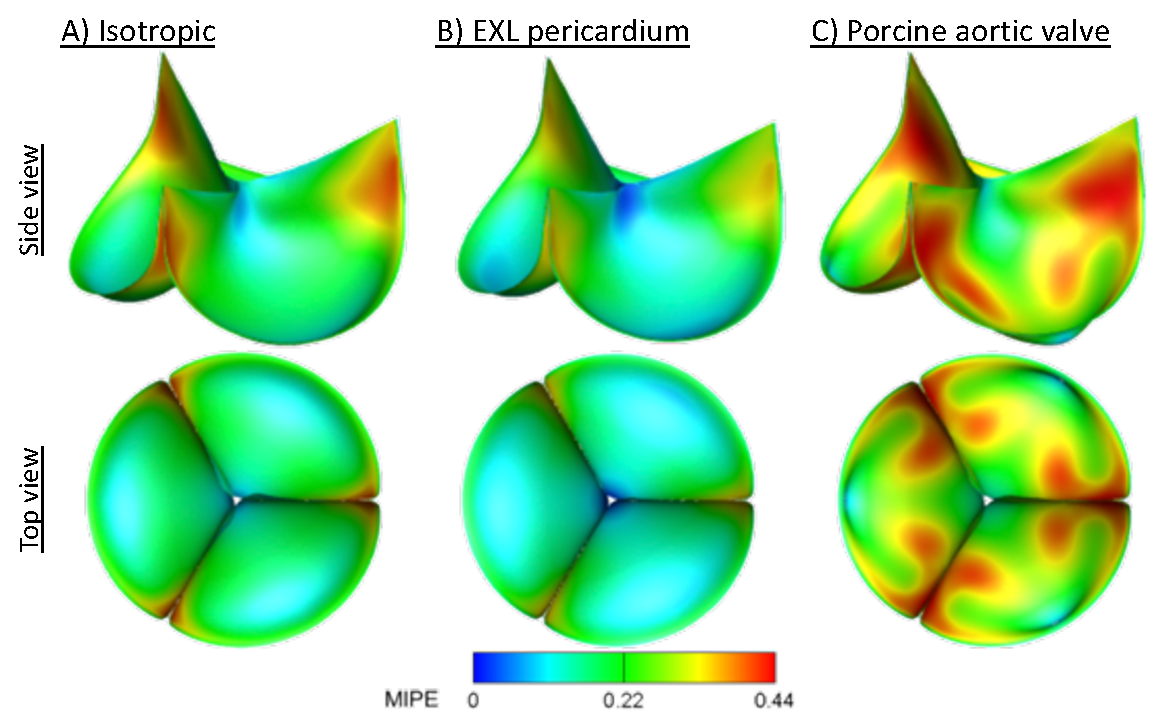
\includegraphics[width=6.5in]{Figures/valvesimulations}
\caption{Simulations of intact tri-leaflet valves using A) the porcine aortic valve properties with an isotropic fiber orientation distribution, B) exogenously cross-linked bovine pericardium properties with the most homogenous stress distribution, and C) the porcine aortic valve properties properties which results in a very heterogeneous stress distribution and the belly region caving in. The top row shows the side view of the valves at 80 mmHg and the bottom row shows the top-down view of the valves at the same transvalvular pressure.}
\label{fig:valvesimulations}
\end{figure}
    
    The material property has significant effects on the mechanical behaviors of the leaflets (Fig. \ref{fig:valvesimulations}). The results are plotted with the maximum in plane Green-Lagrange strain (MIP$\mathbf{E}$). When comparing the three different material, we can see that the native aortic valve properties results in significant heterogeneities in the deformation of the leaflets (Fig. \ref{fig:valvesimulations}C). Specifically, the belly region of the leaflets significantly protrudes out, increasing the load in the surrounding regions, especially near the commissures. This results in some stress concentrations that are not conducive to heart valve durability and health in general. The bovine pericardium valve (Fig. \ref{fig:valvesimulations}B) and the isotropic valve (Fig. \ref{fig:valvesimulations}A) on the other hand has significantly more homogeneous leaflet deformations, especially from the top-down view. Both of these undergoes approximately the same deformation of 0.2 in MIPE. The largest difference between the two is near the commissure regions of the valve. Where the isotropic case is under significantly higher strain. Functionally, the material properties of the exogenously cross-linked bovine pericardium is the most suitable for the valve leaflets, where it more evenly distribute the stresses. 
    
    Much of the reasons behind these differences is likely to be due to the differences between the apparent mechanical properties \textit{in vivo} and the measured mechanical response in the laboratory setting. This is especially true for the properties aortic valve, which is extremely anisotropic with very high compliance in the radial direction of the leaflets. This difference is most likely due to the mismatch of referential configuration between the two state. Residual strain or residual stress has significant impact on the functional properties of the leaflets, specifically the apparent anisotropy and stiffness. Collagen fiber directions and varying regional properties can also have significant impact on the functional properties of the leaflets, and thus the results of the simulation. The valve leaflet shape, root geometry and properties, the arterial or ventricular geometry and loading conditions, can all be significant factors affecting the functions of the valves and in distributing the stress in the leaflets. Furthermore, how these factors affect the fluid dynamics of the valves is also an interesting question, suitable for further study. All in all, this is meant to be a demonstration and proof of concept for using $\Psi_{eff}$ to handle a wide range of soft tissue behaviors and anisotropy for the simulation of biological organs, in this case heart valves. Further and more detailed studies will be reserved for the future.  
  
     
%	To further validate the model, we tested its utility in numerical simulations. Using the Finite Element framework developed by Hsu \textit{et al.}, we implemented the effective constitutive model for simulating tri-leaflet valves. We utilized the heart valve geometry and boundary conditions in Aggarwal and Sacks \cite{aggarwal_inverse_2015} and approximated the effective constitutive model parameters to simulate the quasi-static loading of an intact heart valve. The results are qualitatively compared to those of Aggarwal and Sacks \cite{aggarwal_inverse_2015} for validation.







%\begin{figure}
%\centering
%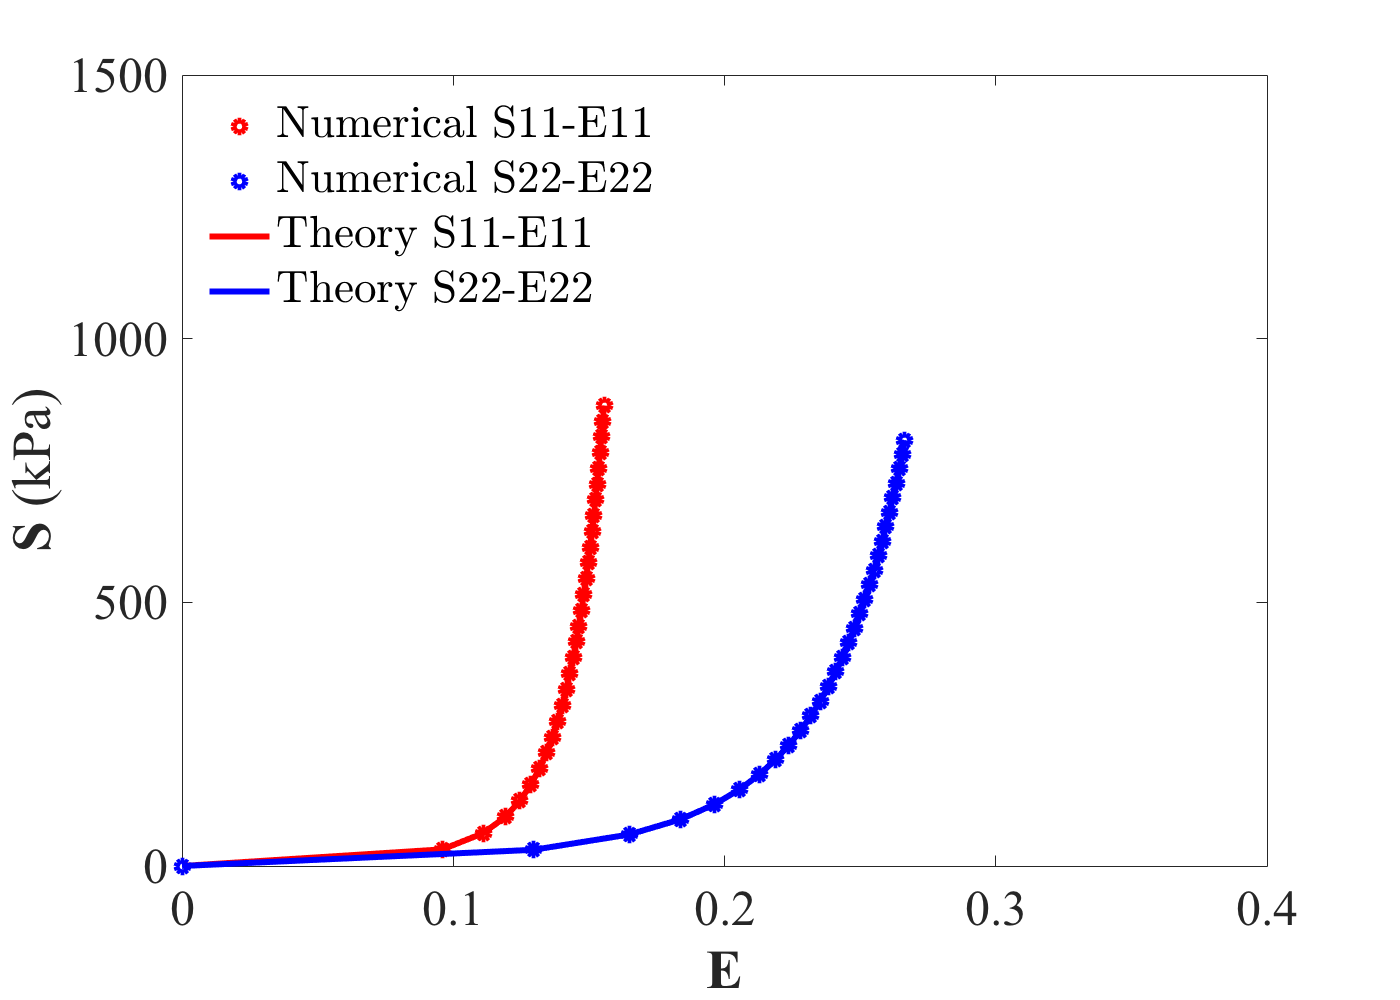
\includegraphics[width=5in]{Figures/validation.png}
%\label{fig:validation}
%\end{figure} 




    



    
    
    
    
    
    
    
    
    
    
    
    
    
    
    



%-----------------------------------------------------------
%	Discussion
%-----------------------------------------------------------

%%%%%%%%%%%%%%%%%%%%%%%%%%%%%%%%%%%%%%%%%%%%%%%%%%%%%%%%%%%%%
%%	Discussion												%
%%%%%%%%%%%%%%%%%%%%%%%%%%%%%%%%%%%%%%%%%%%%%%%%%%%%%%%%%%%%%

\section{Discussion}

%-----------------------------------------------------------
%	Model performance
%-----------------------------------------------------------
\subsection{Reproducing soft tissue response for numerical simulations}

	The most fundamental issue with using phenomenological models for soft tissue and organ numerical simulations are that they 1) cannot simulate deformation beyond the range of data used for parameter estimation, and 2) cannot be widely used for tissues other than the ones they are specifically formulated for. Without being able to fully reproduce the response of micro-models, the resulting response may become inconsistent with the mechanisms of these micro-models, impacting their ability to simulate soft tissue responses, particular when modeling time-dependent processes. In the present work we found that using $\Psi_{eff}$ (Eqn. \ref{eqn:finalexponentialmodelformscaled}) along with optimally selected loading paths reconciles this issue. $\Psi_{eff}$ demonstrates much better capabilities at fitting the mechanical response of soft tissues in general. Admittedly, this may not be especially important for simulations of soft tissues in the normal physiological range as most models can fit the response of tissues if the range of deformation is small, as demonstrated with the generalized Fung model. However, for simulating abnormal conditions such as those that will drastically alters the deformation of the tissue, then using $\Psi_{eff}$ will be much more accurate. 
    
    The second and equally important part is the need for optimal data to determine the model parameters. Admittedly, the amount of data needed is not necessarily extensive. For example, we have shown that just three carefully selected loading paths can greatly improve the predictive capability of $\Psi_{eff}$ over the entire range of deformations. However, when the loading paths are selected poorly, $\Psi_{eff}$ still has some issue when predicting protocol beyond the range used to fit the model. Examples of this are only using a single protocol under equi-biaxial stress (Appendix \ref{sec:otherresults}, Fig. \ref{fig:effequifit}D), or only using protocols in the post-pre-strain range (Fig. \ref{fig:effphypred}). Mechanisms are still the major factor limiting the predictive capability in these cases. However, as the intended role of $\Psi_{eff}$ is to homogenize the response of mechanisms-based micro-models, the loading paths can be simulated by choice, thus should not be a major factor affecting $\Psi_{eff}$ in numerical simulations. 
    
     As we have shown, $\Psi_{eff}$ is able to handle a wide range of soft tissue behavior with no change in model form. This greatly simplifies the need of implementing a different constitutive models for every tissue type, especially when the Jacobian or the elasticity tensor must be implemented separately for computational efficiency, which can be quite complex, i.e. in ABAQUS UMAT. $\Psi_{eff}$ alone is capable of fully reproducing their mechanical response for simulations without significant loss in accuracy. Thus, the use of effective constitutive models can greatly facilitate in not only the computation speed of numerical simulations, but also the speed of implementing constitutive models of different soft tissue for simulations. In these cases, only the parameters of $\Psi_{eff}$ and organ geometry needs to be changed. $\Psi_{eff}$ is smooth, easily differentiable, and easy to implement. With optimal loading path and model scaling, the process of converting micro-model response to $\Psi_{eff}$ (Eqn. \ref{eqn:finalexponentialmodelformscaled}) should take not more than a few seconds, while saving a significant amount of time during numerical simulations. 
     
     On the other hand, micro-models such as the meso-scale structural models are also very useful for reproducing the response of tissue to which the the full microstructure are known. This avoids the need for extensive mechanical data and parameter estimation, saving a time consuming step for evaluating different material designs. Some structural and geometry information may also be measurable \textit{in vivo} due to advances in techniques such as 3D ultrasound \cite{steiner_diagnostic_1994, yang_3d_2008, fenster_3_1996} and DT-MRI \cite{basser_vivo_2000, basser_microstructural_2011}, and can be directly incorporated into meso-scale structural models. However, these techniques do not yet offer sufficient information to directly determine the mechanical properties of tissues. As such, micro-models are still a necessary and important part of any predictive simulation. Not surprisingly, even most traditional invariant based models, such as the Holzapfel-Gasser-Ogden model \cite{holzapfel_new_2000}, are being extended to incorporate the microstructures of the tissue \cite{holzapfel_modelling_2015}. 
    
    


\subsection{Application for the effective constitutive model}
%-------	growth and remodeling	-------%
    
    One application of effective constitutive models is for simulating time-dependent processes, such as growth and remodeling. Growth and remodeling has been a long-time interest of the biomechanics community, and has important role in predictive simulations. Theories for growth and remodeling have been well studied, from Rodriguez in 1994 to Lanir and others in the current time \cite{lanir_mechanistic_2014, gleason_mixture_2004, rodriguez_stress_1994, humphrey_constrained_2002, cowin_tissue_2004, taber_biomechanics_1995}. The general theories for growth and remodeling involves the changes in the reference configurations of the materials and a constrained mixture model involving the combined response of old original materials and new generated materials. The new and old materials are separated into many different parts each with its own material parameters and referential configuration. This again multiplies the computational cost of the material models and the summation of many individual responses can significantly reduce numerical precision. Here homogenization using $\Psi_{eff}$ (Eqn. \ref{eqn:finalexponentialmodelformscaled}) can be useful. 
    

%-------	inverse modeling	-------%
    Another important application is for inverse modeling, which is important for patient specific modeling. Outside of \textit{in vitro} studies, performing the experiments necessary to determine the mechanical response of soft tissues is extremely difficult. Here, inverse modeling approaches are a solution to this problem \cite{lee_inverse_2014, aggarwal_inverse_2015, aggarwal_patient_2013, kim_inverse_2009, liu_inverse_2013}. In inverse modeling, the model parameters and the errors between the simulated and measured strains are simultaneously optimized. However, the available data that can be obtained \textit{in vivo} is limited, and is not always sufficient to accurately determine the model parameters. In these cases, the tissue microstructure can be used along with meso- and multi-scale models to narrow down the range of possible parameters. However, this multiplies the already hefty costs of the these constitutive models, which is complicated by the fact that limited time is available to acquire these model parameters. Here, the approach we proposed (Fig. \ref{fig:simulationframework}B) can be used to reduce computational cost.

%-----------------------------------------------------------
%	Model covariance
%-----------------------------------------------------------
% \subsection{Alternative model forms}

% % 	The standard invariants and pseudo-invariants (Section \ref{sec:invariants}), is not suitable for ours goals for an effective constitutive model. It is more suitable for specific tissue types and is hard to generalize. In some specific cases, such as choosing $I_4 = \vec{M}\cdot\mathbf{C}\vec{M}$, $I_5 = \vec{P}\cdot\mathbf{C}\vec{P}$, and $I_8 = \vec{M}\cdot\mathbf{C}\vec{P}$, $\vec{P}$ orthogonal to $\vec{M}$, you can construct the exact same effective constitutive model, since then $E_m = 1/2(I_4 - 1)$, $E_n = 1/2(I_5 - 1)$, and $E_\phi = 1/2(I_8)$. However, there isn't any point of using invariants if they are restricted to have the same value as the components of strain tensors, this only makes the mathematics more difficult to follow. Using other invariants that are not just just the right Cauchy strain components, can more specifically describe the tissue tissue function. One example is the dual crossing fiber families in arterial tissues. However, this loss in generality is exactly what we want to avoid. What we want is a constitutive model that can fully reproduce the response of a wide range of soft tissue responses. 
    
    
% %     To be fully general, the choice of invariants used in the model really can't be specific to any mechanism or structure. In the end, the 'smallest and complete set of invariants' that can describe any deformation is the strain tensor components themselves. The choices for the strain tensors and conjugate stresses are many, but they are also very similar. The Hencky strains produces the best parameter covariance for constitutive modeling, but this difference is simply not enough to justify using it in place of other strain basis. Likely, there isn't a significant advantage for any specific strain basis in this area. $\mathbf{E}$ is the most convenient for constitutive modeling with the simplest forms for stresses and elasticity tensor (Appendix \ref{sec:elasticitytensor}), thus stands out as the most convenience. 
    

% 	Our first choice for $\Psi_{eff}$ (Eqn. \ref{eqn:finalexponentialmodelformscaled}) is the polynomial series type (Eqn. \ref{eqn:polynomialmodelform}). It has a lot more flexibility for reproducing just about any response. But the number of parameter is too many, and enforcing convexity on the resulting response is too difficult in terms of the number of constraints needed and computational cost added to the model, and parameter estimation. Optimization problems normally taking only 10-20 iterations to converge without constraints, took 200,000 iterations and still did not converge with the constraints added. This process was only stopped after 6 hours by the max iteration value. In such conditions, polynomial series type is clearly not a viable choice. However, we should note that the Hencky strains are extremely beneficial to polynomial series type models, which significantly reduces the parameter correlations (Appendix \ref{sec:parametercorrelation}, Fig. \ref{fig:gvsecorrelationpoly}). Most of the benefits are for the coupling terms in the higher order polynomials. These benefits are greatly reduced for the lower order terms such as those in $\Psi_{eff}$ Although the polynomial series and separated exponential types have lower parameter covariance by separating the individual terms, more coupling terms are needed to fit soft tissue responses, actually increasing the overall covariance of the model. Thus, the disadvantage in parameter covariance in the exponential Q type models is actually less significant overall for parameter estimation. Also, with the model scaling method presented (Section \ref{sec:modelscaling}), parameter covariance does not seem to be an issue for $\Psi_{eff}$. 


%-----------------------------------------------------------
%	Convexity
%-----------------------------------------------------------
\subsection{Convexity}
	
    We did not find any difficulties with enforcing the convexity of $\Psi_{eff}$ (Eqn. \ref{eqn:finalexponentialmodelformscaled}) during parameter estimation. In fact, no constraints were necessary in most cases. Even in the worst scenarios, only a few constraints are required (Eqn. \ref{eqn:effmodelconstraints}). The biggest difficulties with enforcing convexity and ellipticity are the coupling terms such as $E_m^3E_n$ and $E_mE_n^3$. Polynomial series or separated exponential types require many more coupling terms in comparison to $\Psi_{eff}$. Our preliminary testing shows that polynomial model form requires at least 27 terms to fit existing data, 21 of the 27 terms are coupling terms. The resulting constraints are both complex and difficult to enforce. Enforcing convexity and ellipticity on the boundary or any specific points do not guarantee convexity over the entire range. Thus, convexity need to be enforced at separate points within the domain or by integration. This is not only a significant increase in computational costs, as the computational cost of enforcing the constraints vastly exceeds that of the model itself, but also significantly impacts convergence during optimization. The constraint functions are not convex themselves by any means, increasing the number of iterations needed for optimization by several magnitudes more than necessary. In many cases, parameter estimation took 200,000 iterations without convergence after enforcing the constraints, taking over 6 hours by the max iteration value, which is comparable to meso-scale structural approaches with interaction terms \cite{zhang_modeling_2017}(30 min - 4 hours). This makes constrained optimization often intractable to implement, especially in comparison to $\Psi_{eff}$ (Eqn. \ref{eqn:finalexponentialmodelformscaled}) which only takes 5-10 seconds. Thus, the form of $\Psi_{eff}$ proposed is clearly the best choice. 
    

%-----------------------------------------------------------
%	Convergence
%-----------------------------------------------------------
\subsection{Model scaling method and its applications}
    
    Although not introduced as such, the model scaling method, or a similar technique to this, was very actually briefly described by Fung \textit{et al.} in their original work on the mathematical modeling of arteries \cite{fung_pseudoelasticity_1979}. The paper introduced the strain energy density function as 
%==========================================================%
%-------------------	begin EQUATION 	-------------------%
\begin{equation}\label{eqn:fungarterymodel}
\rho_0 W^{(2)} = \frac{C^\prime}{2}\operatorname{exp}\left[\alpha_1 \left(E_{\theta\theta}^2 - E_{\theta\theta}^{*2} \right) + \alpha_2 \left(E_{zz}^2 - E_{zz}^{*2} \right) + \alpha_4 \left(E_{\theta\theta}E_{zz} - E_{\theta\theta}^*E_{zz}^* \right) \right]
\end{equation}
%-------------------	 end EQUATION 	-------------------%
%==========================================================%    
in equation 2 of the said work ($C$ is changed to $C^\prime$ to consistency in notation with the present work). $E_{\theta\theta}^*$ and $E_{zz}^*$ are introduced as strains corresponding to some fixed stresses of $S_{\theta\theta}^*$ and $S_{zz}^*$, usually taken in the physiologic range. Similarly, this "scaling" can be absorbed into the parameter $C^\prime$ like in the present work. This idea was not greatly expanded upon, but \textit{Fung et al.} notes that:
\begin{quotation}
"But in practice it is very helpful to introduce $E_{\theta\theta}^*$ and $E_{zz}^*$. Not only are the values corresponding to $S_{\theta\theta}^*$ and $S_{zz}^*$ very important information, but also their use makes the constants [$C^\prime$], $\alpha_1$, $\alpha_2$, and $\alpha_4$ much more stable for each set of specimen." \cite{fung_pseudoelasticity_1979}
\end{quotation} 
and that 
\begin{quotation}
"[$E_{\theta\theta}^*$ and $E_{zz}^*$] are indexes of compliance of the vessel. Using $E_{\theta\theta}^*$ and $E_{zz}^*$, the variations of the constants $C$, $\alpha_1$, $\alpha_2$, and $\alpha_4$, which determines the shape of the stress-strain curve, are greatly reduced. The assignment of $S_{\theta\theta}^*$ and $S_{zz}^*$ is arbitrary, but hopefully standard values will be adopted by the biomechanics community." \cite{fung_pseudoelasticity_1979}
\end{quotation}

	In truth, we did not find that the model scaling method necessarily makes $\alpha_1$, $\alpha_2$, and $\alpha_4$ more consistent, but rather that they are exactly the same values with or without this method, assuming parameter estimation was not trapped in some local minimum. The model scaling method does make reaching the values of these parameter more consistent. The biggest benefit remains the significant improvement in the correlation between the parameters $C^\prime$ and $\alpha_1$, $\alpha_2$, and $\alpha_4$, improving the topology of the objective function surface during parameter estimation. It also imparts some physical meaning to the value of $C^\prime$, or for $A_s$ and $c_0^\prime$ in present work. For Fung \textit{et al.}, this is some arbitrary physiologic stresses, for us, this is exactly 'maximum' (with respect to the objective function) value of strain energy within the data used for parameter estimation. This does bestow some consistency to the value of $C^\prime$, as it is exactly the total strain energy density at the stresses of $S_{\theta\theta}^*$ and $S_{zz}^*$, which will likely be similar between specimens taken from the same arteries from health subjects. However, the choice of $E_{\theta\theta}^*$ and $E_{zz}^*$, or $E_m^\mathrm{max}$, $E_n^\mathrm{max}$, and $E_\phi^\mathrm{max}$ for $\Psi_{eff}$ (Eqn. \ref{eqn:finalexponentialmodelformscaled}), should not be arbitrary. The model scaling method works due to altering the functional effect of $c_0$ and $b_i$, or $C$ and $\alpha$. $E_m^\mathrm{max}$, $E_n^\mathrm{max}$, and $E_\phi^\mathrm{max}$ should be chosen deliberately so that area under the constitutive model, based on the objective function, remains approximately the same, thus decoupling changes in modulus and changes in curvature from the exponential parameters. 


	Perhaps, the biggest advantage of the model scaling method is that it is applicable to nearly any constitutive model with an exponential function, such as models like the Holzapfel-Gasser-Ogden, Humphrey, Vito, or even the meso-scale structural model with simplified ensemble response such as in Fan and Sacks \cite{fan_simulation_2014a}, Lee \textit{et al.}\cite{lee_effects_2015}, and Aggarwal and Sacks \cite{aggarwal_inverse_2015}. Even polynomial model forms with a power law, $\Psi=A\epsilon^B$, such as the generalized Ogden model, or the elastin model for the mitral valve in Zhang et al. \cite{zhang_meso_2016} can see benefits from the model scaling method. In this case, the scaling term becomes $A = \bar{A} e^{-B \log(\epsilon_{max})}$. In summary, this model scaling method should have significantly implications in improving the speed and consistency of parameter estimation for any model with an exponential like form.
    
    
	
    
%-----------------------------------------------------------
%	Convergence
%-----------------------------------------------------------
\subsection{Convergence rate}

	Typically, we find that parameter estimation converges after 40-60 iterations, although more stringent tolerance may require more iterations for additional digits of precision. We did not observe significant improvements in the rate of convergence in the best-case scenarios, but we also did not observe scenarios which significantly increases the iteration required based on the initial guess like the unscaled traditional forms. We note that the model scaling method does not improve the correlation between the exponent parameters $b_1-b_{13}$ in $Q$, which is a function of the choice of invariants and the terms picked. With that being said, the correlation between the parameters of $Q$ is much better than the correlation between the exponents $b_1-b_{13}$ and modulus $c_0$ (Fig. \ref{fig:gvsecorrelation} and Appendix \ref{sec:parametercorrelation} Table \ref{tb:correlationE} \& \ref{tb:correlationG} vs. Table \ref{tb:ABcorrelation}), it is difficult to further improve the parameter correlation of $Q$ without changing the form of the model. However, for our purpose, this is already sufficient. 

%-----------------------------------------------------------
%	Optimal
%-----------------------------------------------------------
\subsection{Optimal \textit{in silico} loading paths}

	The limitation on predicting outside of the loading paths used for parameter estimation can be somewhat remedied by densely sampling the response of the micro-model over a larger range of deformations. However, this is not entirely ideal for computational speed during parameter estimation, and sampling data points for parameter estimation is not a trivial task itself. Points with high stresses tends to weight heavily during parameter estimation, proper care need to be taken to capture both the high stress and low stress response. Given that the number of data points scales cubically with the separation between data points, this approach is still limited. We will test if using $\Psi_{eff}$ (Eqn. \ref{eqn:finalexponentialmodelformscaled}) along with the use of optimal loading paths can be the solution to this problem. 

	The optimal \textit{in silico} loading paths for parameter estimation and mechanical testing is perhaps very intuitive. The two key factors that should always be consider when sampling data or performing experimental testing are 1) span the as much of the range of deformation as possible and 2) the equibiaxial stress loading path is extremely important. Our optimal design simulations for the loading paths support these views. The equibiaxial stress loading path is always the one shown in figures for most paper, as it gives most intuitively understandable information on the mechanical properties of the tissue. It gives insights into the general form, anisotropy and stiffness of the material at a glance, and is not surprisingly also the best loading path for parameter estimation. Spanning the domain of the possible deformations provides more information for parameter estimation also as expected. However, it is surprising just how little the equibiaxial stress loading path can provide alone. The difference in magnitude between the D-optimality values for one vs. two loading paths is almost 20. The equibiaxial stress alone simply is not enough for accurate parameter estimation of the full response of soft tissues when using $\Psi_{eff}$ (Eqn. \ref{eqn:finalexponentialmodelformscaled}). However, with the addition of one or two more protocols, even if they are along a similar loading paths can significantly improve the predictive capabilities of $\Psi_{eff}$. Reproducing the mechanical response of soft tissues from only fitting the equibiaxial response in figures from papers is unlikely to be sufficient. However, this may be partially overcome by meso-scale structural approaches, given the information on the microstructure of the tissue.  
    
    Having said this, our investigation of optimal loading paths only restricted to constant strain ratios or constant stress ratios. In reality, there are many ways to define loading paths, some can be quite creative. We do not deny the possibility of other forms of loading paths that are more optimal than using stress ratios, but a fully exhaustive search is not an easy problem to tackle and program for optimization. In our search, we restricted the optimization to only the same family of loading paths, defined by only one constant, the ratio of stretch. Even so, the parts of the process is manual, such as increasing the total number of loading paths. Increasing the total number of loading paths was extremely time consuming for most algorithms due to exponentially increasing computational cost (section \ref{sec:optimaldesign}). However, three, or at most five protocols are already sufficient. 
    
    We did test some alternative loading paths, such as Fung \textit{et al.}'s post pre-strain loading paths \cite{fung_pseudoelasticity_1979}. They cover much of the physiological range, but are insufficient for parameter estimation. Increasing the number of loading paths in this case, has minor improvements, but pales in comparison to just picking better types of loading paths. The poor predictive capabilities for the low stress region can have significant impacts on underestimating the mechanical properties of matrix and elastin, and their properties can be important to the functions of micro-models. The mechanical properties of the matrix for example, having significant implications for simulating the process of permanent set in exogenously cross-linked soft tissues \cite{zhang_modeling_2017}. Failing to properly reproduce this response, can affect the predictive capabilities of the associated micro-models, causing the whole framework of using $\Psi_{eff}$ to facilitate numerical simulations (Fig. \ref{fig:simulationframework}B) to fall apart. 
    
    
    
%-----------------------------------------------------------
%	Simulation
%-----------------------------------------------------------
% \subsection{Numerical simulation}
	

 










%-----------------------------------------------------------
%	Conclusion
%-----------------------------------------------------------

%%%%%%%%%%%%%%%%%%%%%%%%%%%%%%%%%%%%%%%%%%%%%%%%%%%%%%%%%%%%%
%%	Conclusion												%
%%%%%%%%%%%%%%%%%%%%%%%%%%%%%%%%%%%%%%%%%%%%%%%%%%%%%%%%%%%%%

% \section{Limitations and conclusion}

%-----------------------------------------------------------
%	Limitations
%-----------------------------------------------------------
\section{Limitations} 
	
    One major limitation of $\Psi_{eff}$ (Eqn. \ref{eqn:finalexponentialmodelformscaled}) is the larger number of parameters, reaching 14 in the fully generalized form and 10 for most specific soft tissue types (Appendix \ref{sec:specificform}). This is not very favorable, where the time complexity for most optimization algorithms scales nonlinearly with the number of parameters. However, $\Psi_{eff}$ has very low computational cost, and reasonable low parameter covariance, thus this should not be a major problem. Alternatives are also less favorable, as they either require more parameters or cannot sufficiently capture the response of soft tissues in a large range or reproduce the response of multiple tissue types. 
    
    Another limitations, which also applies for all phenomenological models, is that $\Psi_{eff}$ has no intrinsic mechanisms built in. Without sufficient mechanical data to derive the model parameters, phenomenological models generalize have limited predictive capabilities. Specifically, the phenomenological models does poorly when extrapolating outside of the range of data. This also means that phenomenological models can only provide limited information on how the tissue functions. It can reproduce the mechanical response of soft tissues very well, but it is also harder to infer more about the structure and function of the tissue. This is not a major concern for us. For the mechanisms, or the structure to function relationship of soft tissues, micro-models already fulfills the need. $\Psi_{eff}$ is intended as a fit all model for fulfilling the gap between predictive micro-models and computationally efficient simulations. With carefully selected of loading paths for parameter estimation (Section \ref{sec:optimaldesign}), $\Psi_{eff}$ can accurately reproduce the mechanical response of soft tissue within the expected range. In other words, $\Psi_{eff}$ does not have to be able to predict the mechanical response of soft tissues under unmeasured and extrapolated deformations, it only have to be able to fully reproduce the entire range of responses predicted by the micro-models, which is its main purpose. 



%-----------------------------------------------------------
%	Conclusion
%-----------------------------------------------------------
\section{Conclusion and Future Directions} 

	In this work, we developed a constitutive model form for the effective response of planar soft tissues. This effective constitutive model (Eqn. \ref{eqn:finalexponentialmodelformscaled}) is applicable to a wide range of soft tissue responses, while being as computationally efficient as most common phenomenological approaches, such as Holzapfel-Gasser-Ogden or the generalized Fung model. This model utilizes the modeling scaling method for minimally covariant parameter, which shows significant improvements in the speed and accuracy of parameter estimation. We have shown that our effective constitutive model along with optimal loading paths is able to fully replicate the response of complex meso-scale structural models for the entire range of deformations, where most phenomenological models have difficulties when predicting unfitted loading paths. The effective constitutive model is robust enough to be able to handle a wide range of soft tissue behaviors and anisotropy for accurate numerical simulations, such as in simulations of heart valves. Thus, the effective constitutive model can play an important role for the upscaling and homogenization of the response of complex micro-models for improving the efficiency for organ-level simulations, as well as further extensions for time-dependent processes. 
    

	One nature extension to this effective modeling approach is for 3 dimensional soft tissues. The extension to 3 dimensions doubles the number of inputs in comparison to planar models, with the additional inputs being $E_{13}$, $E_{23}$, and $E_{33}$. This means that the initial most generalized form for the 3-D soft tissue models (Eqn. \ref{eqn:exponentialmodelform}) has 209 terms before reduction. This is unmanageable for establishing the initial approach, where using a planar soft tissue model is more suitable. However, applying the same restrictions to the model form (section \ref{sec:finalform}) reduces this to 48 terms. This is possible due to symmetry by expressing the components of the Green-Lagrange strain tensor with respect to the material axis (Eqn. \ref{eqn:greenstrain}). This is not so easy to do in 3-dimensions, requiring a third vector corresponding to the direction of least stiffness, which in turn requires the 3 dimensional fiber orientation distribution. 
    
    
    
    
    
    
    
    


%-----------------------------------------------------------
%	Acknowledgements
%-----------------------------------------------------------

% \begin{acknowledgment}
% This work is in thanks for the support from NIH grants: 
%   HL-068816, HL-089750, HL-070969, and HL-108330 
% \end{acknowledgment}

\section*{Acknowledgements}
This work is in thanks for the support from NIH grants: 
  HL-068816, HL-089750, HL-070969, and HL-108330 

%-----------------------------------------------------------
%	Nomenclature
%-----------------------------------------------------------
\newpage
%%%%%%%%%%%%%%%%%%%%%%%%%%%%%%%%%%%%%%%%%%%%%%%%%%%%%%%%%%%%%
%%  nomenclature											%
%%%%%%%%%%%%%%%%%%%%%%%%%%%%%%%%%%%%%%%%%%%%%%%%%%%%%%%%%%%%%

%-----------------------------------------------------------
%	Symbols
%-----------------------------------------------------------
\nomenclature[S,01]{$s$}{Scalar variables}
\nomenclature[S,02]{$\mathbf{v}$}{Vector variables, bold lower case}
\nomenclature[S,03]{$\mathbf{M}$}{Matrix variables, bold upper case}
\nomenclature[S,04]{$\hat{\Psi},\hat{S},\hat{f}$}{Data}
\nomenclature[S,05]{$\mathbf{I}$}{Identity tensor}
\nomenclature[S,06]{$J$}{The Jacobian for volume change due to deformation}
\nomenclature[S,07]{$\mathbf{F}$}{The deformation gradient tensor}
\nomenclature[S,08]{$\mathbf{f}$}{The upper triangular decomposition of the deformation gradient tensor}
\nomenclature[S,09]{$\mathbf{C}$}{Right Cauchy-Green strain tensor}
\nomenclature[S,10]{$\mathbf{B}$}{Left Cauchy-Green strain tensor}
\nomenclature[S,11]{$\mathbf{E}$}{Green Lagrange strain}
\nomenclature[S,12]{$\mathbf{U}$}{Right stretch tensor}
\nomenclature[S,13]{$\mathbf{T}$}{The Cauchy stress tensor}
\nomenclature[S,14]{$\mathbf{S}$}{Second Piola Kirchhoff tensor}
\nomenclature[S,15]{$I_1$}{First invariant of the right Cauchy strain tensor}
\nomenclature[S,16]{$I_2$}{Second invariant of the right Cauchy strain tensor}
\nomenclature[S,17]{$I_3$}{Third invariant of the right Cauchy strain tensor}
\nomenclature[S,18]{$I_4$}{Fourth pseudo-invariant of the right Cauchy strain tensor describing the stretch along an axis}
\nomenclature[S,19]{$I_8$}{Eighth pseudo invariant, describing the relative stretch along two axes}
\nomenclature[S,20]{$I_8^{ext}$}{The extensional component of $I_8$ }
\nomenclature[S,21]{$\mathbf{m}_0$}{The material axis in the reference configuration}
\nomenclature[S,22]{$\mathbf{n}_0$}{The perpendicular axis to the material axis in the reference configuration}
\nomenclature[S,23]{$\mathbf{m}_t$}{The material axis in the deformed configuration}
\nomenclature[S,24]{$\mathbf{n}_t$}{The perpendicular axis to the material axis in the deformed configuration}
\nomenclature[S,25]{$\lambda_m$}{The stretch along the material axis}
\nomenclature[S,26]{$\lambda_n$}{The stretch perpendicular to the material axis}
\nomenclature[S,27]{$\phi$}{The shear angle between $\mathbf{m}_0$ and $\mathbf{n}_0$}
\nomenclature[S,28]{$E_m, E_n, E_\phi$}{The Green Lagrange strain along the respective axes and to shearing}
\nomenclature[S,29]{$S_m, S_n, S_\phi$}{The 2nd Piola Kirchhoff stress along the respective axes and to shearing, which are also response functions, gradients of the strain energy}
\nomenclature[S,30]{$\gamma_1,\gamma_2,\gamma_3$}{The Hencky strains}
\nomenclature[S,31]{$\Psi$}{The strain energy}
\nomenclature[S,32]{$\Psi_\mathrm{col}, \Psi_\mathrm{int}, \Psi_\mathrm{mat}$}{Strain energy of the collagen fiber, ensemble-ensemble interactions, and matrix components respectively}
\nomenclature[S,33]{$\eta_C$, $\eta_M$, $\eta_I$}{The modulus of collagen, matrix and fiber-fiber interactions}
\nomenclature[S,34]{$\phi_\mathrm{col}$, $\phi_\mathrm{mat}$, $\phi_\mathrm{int}$}{The mass fractions of collagen, matrix and fiber-fiber interactions}
\nomenclature[S,35]{$D$}{Collagen fiber recruitment distribution function}
\nomenclature[S,36]{$\Gamma$}{Collagen fiber orientation distribution function}
\nomenclature[S,37]{$\lambda$}{Stretch}
\nomenclature[S,38]{$\lambda_s$}{The slack stretch, the stretch needed to straighten the collagen fiber crimp}
\nomenclature[S,39]{$\mathcal{F}$}{Objective function for parameter estimation}
\nomenclature[S,40]{$\mathbfcal{I}$}{The information matrix}
\nomenclature[S,41]{$\mathbf{J}$}{The Jacobian of the objective function}
\nomenclature[S,42]{$\mathbfcal{H}$}{The Hessian of the objective function}
\nomenclature[S,43]{$\mathbf{\xi}$}{Vector of material parameters}



%-----------------------------------------------------------
%	Key Terms
%-----------------------------------------------------------
\nomenclature[K,1]{\it Phenomenological model}{Constitutive models that reproduces the mechanical response of materials without taking into considerations any underlying structure or mechanisms}
\nomenclature[K,2]{\it Micro-models}{Constitutive models utilizing structures and mechanism at a lower scale to predict the mechanical response at a higher scale}
\nomenclature[K,3]{\it Structural model}{Constitutive models that utilize the meso-scale microstructures to predict the mechanical response of soft tissues}
\nomenclature[K,4]{\it Effective constitutive model}{A computationally phenomenological model used to reproduce the response of micro material models in numerical simulations}
\nomenclature[K,5]{\it Polynomial series family}{Effective model forms composed primarily of sums of polynomial functions}
\nomenclature[K,6]{\it Separated exponential family}{Effective model forms composed primarily of sums of exponential functions}
\nomenclature[K,7]{\it Single exponential family}{Effective model forms composed primarily of a single exponential function of sums of polynomial functions}
\nomenclature[K,8]{\it ODF}{Orientation distribution function}
\nomenclature[K,9]{\it RDF}{Recruitment distribution function, the distribution of stretched needed to straighten the collagen fibers}
\nomenclature[K,10]{\it Physiologic range}{The range of deformations most likely to contain the physiologic loading path}





\printnomenclature







%-----------------------------------------------------------
%	References
%-----------------------------------------------------------
\newpage
\section*{References}

\bibliography{WCCMS,ccsdifference}

%-----------------------------------------------------------
%	Appendix
%-----------------------------------------------------------
%\appendix
\newpage
% \renewcommand{\theequation}{\thechapter.\arabic{equation}}
\begin{appendices}

\renewcommand\thefigure{\thesection.\arabic{figure}}    
\renewcommand\thetable{\thesection.\arabic{table}}   
\renewcommand\theequation{\thesection.\arabic{equation}}

\setcounter{figure}{0}
\setcounter{equation}{0}
\section{Elasticity tensor}\label{sec:elasticitytensor}

	An analytical form for the elasticity tensor is extremely important for fast and convergent numerical simulations. A constitutive model without a smooth, continuous, and convex elasticity tensor can pose significant problems for simulation of nonlinear materials to converge quickly, or even to converge at all. The strain basis used for the model can have significant impact on the form of the elasticity tensor. Here, we derived the generalized form of the elasticity tensor for using the Green-Lagrange basis (Eqn. \ref{eqn:greenstrain}) and the Hencky strain basis (Eqn. \ref{eqn:henckystrains}). Note that this is the generalized form, which does not depend on the explicit form of the constitutive model, it is only a function of the strain basis and the response functions (derivatives of the strain energy function), whose form doesn't not have to be explicitly stated. The 9 response functions are:
%=======	BEGIN Equation		=======%
\begin{equation}
\dpd{\Psi}{E_m}, \quad \dpd{\Psi}{E_n}, \quad \dpd{\Psi}{E_\phi}, \quad \frac{\partial^2\Psi}{\partial E_m^2}, \quad \frac{\partial^2\Psi}{\partial E_n^2}, \quad \frac{\partial^2\Psi}{\partial E_\phi^2}, \quad \frac{\partial^2\Psi}{\partial E_m\partial E_n}, \quad \frac{\partial^2\Psi}{\partial E_m\partial E_\phi}, \quad \frac{\partial^2\Psi}{\partial E_n\partial E_\phi}.
\end{equation}
%=======	END Equation		=======%
    
\subsection{Derivation with Green-Lagrange strain}
	
    The elasticity tensor is given by the second derivative of the strain energy function with respect to the right Cauchy strain. Using the chain rules, fully expanding all terms, and enforcing symmetry of partial derivatives, $\md{\Psi}{2}{E_m}{}{E_n}{} = \md{\Psi}{2}{E_n}{}{E_m}{}$, the generalized form for the elasticity tensor is given by 
%=======	BEGIN Equation		=======%
\begin{equation} \label{eqn:generalizedelasticityform}
\begin{aligned}
\dod[2]{\Psi}{\mathbf{C}} =& 
	\dpd{\Psi}{E_m} \dod[2]{E_m}{\mathbf{C}} 
    + \dpd{\Psi}{E_n} \dod[2]{E_n}{\mathbf{C}}
    + \dpd{\Psi}{E_\phi} \dod{E_\phi}{\mathbf{C}} \\
+& \dpd[2]{\Psi}{E_m} \dod{E_m}{\mathbf{C}}\dod{E_m}{\mathbf{C}} 
	+ \dpd[2]{\Psi}{E_n} \dod{E_n}{\mathbf{C}} \dod{E_n}{\mathbf{C}} 
    + \dpd{\Psi}{E_\phi} \dod{E_\phi}{\mathbf{C}} \dod{E_\phi}{\mathbf{C}} \\
+& \dmd{\Psi}{2}{E_m}{}{E_n}{} \left(\dod{E_n}{\mathbf{C}} \dod{E_m}{\mathbf{C}} + \dod{E_m}{\mathbf{C}} \dod{E_n}{\mathbf{C}}\right)   \\
    +& \dmd{\Psi}{2}{E_m}{}{E_\phi}{} \left(\dod{E_\phi}{\mathbf{C}} \dod{E_m}{\mathbf{C}} + \dod{E_m}{\mathbf{C}} \dod{E_\phi}{\mathbf{C}}\right)  \\
    +& \dmd{\Psi}{2}{E_n}{}{E_\phi}{} \left(\dod{E_n}{\mathbf{C}} \dod{E_\phi}{\mathbf{C}} + \dod{E_\phi}{\mathbf{C}} \dod{E_n}{\mathbf{C}}\right).  \\
\end{aligned}
\end{equation}
%=======	END Equation		=======%
To break this down, we begin with the derivatives of the Green-Lagrange strains, which are given by,
%==========================================================%
%-------------------	begin EQUATION 	-------------------%
\begin{equation}\label{eqn:partialgreens}
\begin{aligned}
\dod{E_m}{\mathbf{C}} &= \frac{1}{2} \mathbf{m}\otimes\mathbf{m}	\\
\dod{E_n}{\mathbf{C}} &= \frac{1}{2} \mathbf{n}\otimes\mathbf{n} \\
\dod{E_\phi}{\mathbf{C}} &= \frac{1}{4} \left(\mathbf{m}\otimes\mathbf{n} + \mathbf{n}\otimes\mathbf{m} \right),
\end{aligned}
\end{equation}
%-------------------	 end EQUATION 	-------------------%
%==========================================================%
and 
%==========================================================%
%-------------------	begin EQUATION 	-------------------%
\begin{equation}
\dod[2]{E_m}{\mathbf{C}} = \dod[2]{E_n}{\mathbf{C}} = \dod[2]{E_\phi}{\mathbf{C}} = \mathbf{0}.
\end{equation}
%-------------------	 end EQUATION 	-------------------%
%==========================================================%
Right away, the Green-Lagrange strains have the benefit of the second derivatives being zero, reducing the elasticity tensor (Eqn. \ref{eqn:generalizedelasticityform}) from 9 to 6 terms. Substituting with the partial derivatives (Eqn. \ref{eqn:partialgreens}) gives
%==========================================================%
%-------------------	begin EQUATION 	-------------------%
\begin{equation}\label{eqn:greenelasticityform}
\begin{aligned}
\dod[2]{\Psi}{\mathbf{C}} =
	& \frac{1}{4}\dpd[2]{\Psi}{E_m} \mathbf{m}\otimes\mathbf{m}\otimes\mathbf{m}\otimes\mathbf{m}	\\
    &+ \frac{1}{8}\dmd{\Psi}{2}{E_m}{}{E_\phi}{} 
    	\left(
        	\mathbf{m}\otimes\mathbf{m}\otimes\mathbf{m}\otimes\mathbf{n}
            +\mathbf{m}\otimes\mathbf{m}\otimes\mathbf{n}\otimes\mathbf{m}
            +\mathbf{m}\otimes\mathbf{n}\otimes\mathbf{m}\otimes\mathbf{m}
            +\mathbf{n}\otimes\mathbf{m}\otimes\mathbf{m}\otimes\mathbf{m}
        \right)	\\
    &+ \frac{1}{4}\dmd{\Psi}{2}{E_m}{}{E_n}{} 
    	\left(
        	\mathbf{m}\otimes\mathbf{m}\otimes\mathbf{n}\otimes\mathbf{n}
            +\mathbf{n}\otimes\mathbf{n}\otimes\mathbf{m}\otimes\mathbf{m}
        \right)	\\
    &+ \frac{1}{16}\dpd[2]{\Psi}{E_\phi} 
    	\left(
        	\mathbf{m}\otimes\mathbf{n}\otimes\mathbf{m}\otimes\mathbf{n}
            +\mathbf{m}\otimes\mathbf{n}\otimes\mathbf{n}\otimes\mathbf{m}
            +\mathbf{n}\otimes\mathbf{m}\otimes\mathbf{m}\otimes\mathbf{n}
            +\mathbf{n}\otimes\mathbf{m}\otimes\mathbf{n}\otimes\mathbf{m}
        \right)	\\
    &+ \frac{1}{8}\dmd{\Psi}{2}{E_n}{}{E_\phi}{} 
    	\left(
        	\mathbf{m}\otimes\mathbf{n}\otimes\mathbf{n}\otimes\mathbf{n}
            +\mathbf{n}\otimes\mathbf{m}\otimes\mathbf{n}\otimes\mathbf{n}
            +\mathbf{n}\otimes\mathbf{n}\otimes\mathbf{m}\otimes\mathbf{n}
            +\mathbf{n}\otimes\mathbf{n}\otimes\mathbf{n}\otimes\mathbf{m}
        \right)	\\
    &+ \frac{1}{4} \dpd[2]{\Psi}{E_n} \mathbf{n}\otimes\mathbf{n}\otimes\mathbf{n}\otimes\mathbf{n}	\\
\end{aligned}
\end{equation}
%-------------------	 end EQUATION 	-------------------%
%==========================================================%


\subsection{Derivation with Hencky strains}

	The elasticity tensor when using the Hencky strains is much more complex. For start, the second derivatives of the Hencky strains are non-zero. The derivatives themselves are complex both in form and conceptually. The derivation of the derivatives is not straight forward. To make this simpler, we start with an alternative definition for the Hencky strains, which relates the 4 variables, $\gamma_1$, $\gamma_2$, $\gamma_3$, and $\mathbf{C}$.  
%==========================================================%
%-------------------	begin EQUATION 	-------------------%
\begin{equation}\label{eqn:invariantset}
\begin{aligned}
    \gamma_1 &= \ln \left( \lambda_m \right), &  \lambda_m^2 &= \mathbf{m}\cdot\mathbf{C}\mathbf{m}  \\
    \gamma_2 &= \ln \left( \lambda_n \right), &  \lambda_n^2 &= \mathbf{n}\cdot\mathbf{C}\mathbf{n} 
                    - \lambda_m^2 \phi^2   \\
    \gamma_3 &= \phi, & \phi &= \left( \lambda_m\right)^{-2}\mathbf{m}\cdot\mathbf{C}\mathbf{n}.
\end{aligned}
\end{equation}
%-------------------	 end EQUATION 	-------------------%
%==========================================================%
It is important here that with this definition, the vector basis, $\mathbf{m}$ and $\mathbf{n}$, are defined on the reference coordinate system, which does not change with deformation. By chain rule, the first derivatives are as followed,
%==========================================================%
%-------------------	begin EQUATION 	-------------------%
\begin{subequations}
\begin{align}
\dod{\gamma_1}{\mathbf{C}} =& \dpd{\gamma_1}{\lambda_m}\dod{\lambda_m}{\mathbf{C}},	
	& \dod{\lambda_m^2}{\mathbf{C}} =& \dpd{\lambda_m^2}{\mathbf{C}}:\dod{\mathbf{C}}{\mathbf{C}} 
	+ \dpd{\lambda_m^2}{\lambda_n}\dod{\lambda_n}{\mathbf{C}}
    + \dpd{\lambda_m^2}{\phi}\dod{\phi}{\mathbf{C}} \\
\dod{\gamma_2}{\mathbf{C}} =& \dpd{\gamma_2}{\lambda_n}\dod{\lambda_n}{\mathbf{C}},	
	& \dod{\lambda_n^2}{\mathbf{C}} =& \dpd{\lambda_n^2}{\mathbf{C}}:\dod{\mathbf{C}}{\mathbf{C}} 
	+ \dpd{\lambda_n^2}{\lambda_m}\dod{\lambda_m}{\mathbf{C}}
    + \dpd{\lambda_n^2}{\phi}\dod{\phi}{\mathbf{C}} \\
\dod{\gamma_3}{\mathbf{C}} =& \dod{\phi}{\mathbf{C}},
	& \dod{\phi}{\mathbf{C}} =& \dpd{\phi}{\mathbf{C}}:\dod{\mathbf{C}}{\mathbf{C}} 
	+ \dpd{\phi}{\lambda_m}\dod{\lambda_m}{\mathbf{C}}
    + \dpd{\phi}{\lambda_n}\dod{\lambda_n}{\mathbf{C}}. 
\end{align}
\end{subequations}
%-------------------	 end EQUATION 	-------------------%
%==========================================================%
First, note that all the partial derivatives are functions of each other. This is indeed problematic, but also note from equation \ref{eqn:invariantset} that $\lambda_m$ does not depend on $\lambda_2$ and $\phi$, and $\phi$ does not depend on $\lambda_2$. This means that the following partial derivatives are zero,
%==========================================================%
%-------------------	begin EQUATION 	-------------------%
\begin{equation}\label{eqn:henckystraindependence}
\begin{aligned}
\dpd{\lambda_m}{\lambda_n} = \dpd{\lambda_m}{\phi} = \dpd{\phi}{\lambda_n} = 0,
\end{aligned}
\end{equation}
%-------------------	 end EQUATION 	-------------------%
%==========================================================%
allowing the equations to be solved. 

	For the second derivatives, note from the definition we have above, the Hencky strains are only linear function of $\mathbf{C}$, thus their 2nd \emph{partial derivatives} are zero with respect to $\mathbf{C}$ only,
%==========================================================%
%-------------------	begin EQUATION 	-------------------%
\begin{equation}
\begin{aligned}
\dpd{}{\mathbf{C}}\left(\dod{\gamma_1}{\mathbf{C}}\right) 
	=\dpd{}{\mathbf{C}}\left(\dod{\gamma_2}{\mathbf{C}}\right)
    =\dpd{}{\mathbf{C}}\left(\dod{\gamma_3}{\mathbf{C}}\right)
    =0.
\end{aligned}
\end{equation}
%-------------------	 end EQUATION 	-------------------%
%==========================================================%
The second derivatives are thus defined to be,
%==========================================================%
%-------------------	begin EQUATION 	-------------------%
\begin{subequations}
\begin{align}
\dod{}{\mathbf{C}}\left(\dod{\gamma_1}{\mathbf{C}}\right) =&
    \dpd{}{\lambda_m}\left(\dod{\gamma_1}{\mathbf{C}}\right)\dod{\lambda_m}{\mathbf{C}}
    + \dpd{}{\lambda_n}\left(\dod{\gamma_1}{\mathbf{C}}\right)\dod{\lambda_n}{\mathbf{C}}
    + \dpd{}{\phi}\left(\dod{\gamma_1}{\mathbf{C}}\right)\dod{\phi}{\mathbf{C}}	\\
\dod{}{\mathbf{C}}\left(\dod{\gamma_2}{\mathbf{C}}\right) =&
    \dpd{}{\lambda_m}\left(\dod{\gamma_2}{\mathbf{C}}\right)\dod{\lambda_m}{\mathbf{C}}
    + \dpd{}{\lambda_n}\left(\dod{\gamma_2}{\mathbf{C}}\right)\dod{\lambda_n}{\mathbf{C}}
    + \dpd{}{\phi}\left(\dod{\gamma_2}{\mathbf{C}}\right)\dod{\phi}{\mathbf{C}}	\\
\dod{}{\mathbf{C}}\left(\dod{\phi}{\mathbf{C}}\right) =&
    \dpd{}{\lambda_m}\left(\dod{\phi}{\mathbf{C}}\right)\dod{\lambda_m}{\mathbf{C}}
    + \dpd{}{\lambda_n}\left(\dod{\phi}{\mathbf{C}}\right)\dod{\lambda_n}{\mathbf{C}}
    + \dpd{}{\phi}\left(\dod{\phi}{\mathbf{C}}\right)\dod{\phi}{\mathbf{C}} 
\end{align}
\end{subequations}
%-------------------	 end EQUATION 	-------------------%
%==========================================================%
Taking advantage of equation \ref{eqn:henckystraindependence}, the first and second derivatives of the Hencky strains are presented as followed:
%==========================================================%
%-------------------	begin EQUATION 	-------------------%
\begin{subequations} \label{eqn:henckyderivatives}
\begin{align}
\dod{\gamma_1}{\mathbf{C}} =& \frac{1}{2\lambda_m^2} \mathbf{m}\otimes\mathbf{m}	\\
\dod{\gamma_2}{\mathbf{C}} =& \frac{1}{2\lambda_n^2} \left(\mathbf{n}\otimes\mathbf{n} - \phi \left( \mathbf{m}\otimes\mathbf{n} + \mathbf{n}\otimes\mathbf{m}\right) + \phi^2 \mathbf{m}\otimes\mathbf{m} \right)	\\
\dod{\gamma_3}{\mathbf{C}} =& \frac{1}{2\lambda_m^2} \left( \mathbf{m}\otimes\mathbf{n} + \mathbf{n}\otimes\mathbf{m} - 2\phi \mathbf{m}\otimes\mathbf{m}\right) \\
\dod[2]{\gamma_1}{\mathbf{C}} =& -\frac{1}{2}\frac{1}{\lambda_m^4}\mathbf{m}\otimes\mathbf{m} \otimes \mathbf{m}\otimes\mathbf{m}	\\
\begin{split}
\dod[2]{\gamma_2}{\mathbf{C}} =& -\frac{1}{2}\frac{1}{\lambda_n^4} 
    \left[
    \mathbf{n}\otimes\mathbf{n}\otimes\mathbf{n}\otimes\mathbf{n}
    -\phi \mathbf{m}\otimes\mathbf{n}\otimes\mathbf{n}\otimes\mathbf{n}
    -\phi \mathbf{n}\otimes\mathbf{m}\otimes\mathbf{n}\otimes\mathbf{n}\right.   \\
    &-\phi \mathbf{n}\otimes\mathbf{n}\otimes\mathbf{m}\otimes\mathbf{n}
    -\phi \mathbf{n}\otimes\mathbf{n}\otimes\mathbf{n}\otimes\mathbf{m}   
    +\phi^2 \mathbf{m}\otimes\mathbf{m}\otimes\mathbf{n}\otimes\mathbf{n} \\
    &\left.+\phi^2 \mathbf{n}\otimes\mathbf{n}\otimes\mathbf{m}\otimes\mathbf{m}
    \right]\\
    &-\left(\frac{1}{4}\frac{1}{\lambda_m^2\lambda_n^2} + \frac{1}{2}\phi^2\frac{1}{\lambda_n^4} \right)
    \left[
    \mathbf{m}\otimes\mathbf{n}\otimes\mathbf{m}\otimes\mathbf{n}
    +\mathbf{m}\otimes\mathbf{n}\otimes\mathbf{n}\otimes\mathbf{m} \right. \\
    &+\left. \mathbf{n}\otimes\mathbf{m}\otimes\mathbf{m}\otimes\mathbf{n}
    +\mathbf{n}\otimes\mathbf{m}\otimes\mathbf{n}\otimes\mathbf{m}
    \right]\\
    &+\left(\frac{1}{2}\phi\frac{1}{\lambda_m^2\lambda_n^2} + \frac{1}{2}\phi^3\frac{1}{\lambda_n^4} \right)
    \left[
    \mathbf{m}\otimes\mathbf{m}\otimes\mathbf{m}\otimes\mathbf{n}
    +\mathbf{m}\otimes\mathbf{m}\otimes\mathbf{n}\otimes\mathbf{m} \right. \\
    &+\left. \mathbf{m}\otimes\mathbf{n}\otimes\mathbf{m}\otimes\mathbf{m}
    +\mathbf{n}\otimes\mathbf{m}\otimes\mathbf{m}\otimes\mathbf{m}
    \right]\\
    &-\left(\phi^2\frac{1}{\lambda_m^2\lambda_n^2} + \frac{1}{2}\phi^4\frac{1}{\lambda_n^4} \right)
    \left[
    \mathbf{m}\otimes\mathbf{m}\otimes\mathbf{m}\otimes\mathbf{m}
    \right]
\end{split}\\
\begin{split}
\dod[2]{\gamma_3}{\mathbf{C}} =& -\frac{1}{2}\frac{1}{\lambda_m^4} \times \left(
        \mathbf{n}\otimes\mathbf{m}\otimes\mathbf{m}\otimes\mathbf{m} + \mathbf{m}\otimes\mathbf{n}\otimes\mathbf{m}\otimes\mathbf{m}\right. \\
        &+ \left.\mathbf{m}\otimes\mathbf{m}\otimes\mathbf{n}\otimes\mathbf{m} +
        \mathbf{m}\otimes\mathbf{m}\otimes\mathbf{m}\otimes\mathbf{n} - 
        4\phi\mathbf{m}\otimes\mathbf{m} \otimes \mathbf{m}\otimes\mathbf{m} \right)
\end{split}
\end{align}
\end{subequations}
%-------------------	 end EQUATION 	-------------------%
%==========================================================%

	Saving everyone from the algebra, without further ado, the most elegant form of the elasticity tensor for constitutive models based on the Hencky strains is, 
%==========================================================%
%-------------------	begin EQUATION 	-------------------%
\begin{subequations} \label{eqn:elasticityhencky}
\begin{align}
\begin{split}
\dod[2]{\Psi}{\mathbf{C}} =&
	\psi_1 \mathbf{m}\otimes\mathbf{m}\otimes\mathbf{m}\otimes\mathbf{m}	\\
    &+ \psi_2
    	\left(
        	\mathbf{m}\otimes\mathbf{m}\otimes\mathbf{m}\otimes\mathbf{n}
            +\mathbf{m}\otimes\mathbf{m}\otimes\mathbf{n}\otimes\mathbf{m}
            +\mathbf{m}\otimes\mathbf{n}\otimes\mathbf{m}\otimes\mathbf{m}
            +\mathbf{n}\otimes\mathbf{m}\otimes\mathbf{m}\otimes\mathbf{m}
        \right)	\\
    &+ \psi_3
    	\left(
        	\mathbf{m}\otimes\mathbf{m}\otimes\mathbf{n}\otimes\mathbf{n}
            +\mathbf{n}\otimes\mathbf{n}\otimes\mathbf{m}\otimes\mathbf{m}
        \right)	\\
    &+ \psi_4
    	\left(
        	\mathbf{m}\otimes\mathbf{n}\otimes\mathbf{m}\otimes\mathbf{n}
            +\mathbf{m}\otimes\mathbf{n}\otimes\mathbf{n}\otimes\mathbf{m}
            +\mathbf{n}\otimes\mathbf{m}\otimes\mathbf{m}\otimes\mathbf{n}
            +\mathbf{n}\otimes\mathbf{m}\otimes\mathbf{n}\otimes\mathbf{m}
        \right)	\\
    &+ \psi_5
    	\left(
        	\mathbf{m}\otimes\mathbf{n}\otimes\mathbf{n}\otimes\mathbf{n}
            +\mathbf{n}\otimes\mathbf{m}\otimes\mathbf{n}\otimes\mathbf{n}
            +\mathbf{n}\otimes\mathbf{n}\otimes\mathbf{m}\otimes\mathbf{n}
            +\mathbf{n}\otimes\mathbf{n}\otimes\mathbf{n}\otimes\mathbf{m}
        \right)	\\
    &+ \psi_6 \mathbf{n}\otimes\mathbf{n}\otimes\mathbf{n}\otimes\mathbf{n}
\end{split}	\\
\begin{split}
\psi_1 =&
        -\frac{1}{2}\frac{1}{\lambda_m^4}W^{(1)}
        -\left(\frac{\phi^2}{\lambda_m^2\lambda_n^2}+\frac{1}{2}\frac{\phi^4}{\lambda_n^4}\right)W^{(2)}
        +2\frac{\phi}{\lambda_m^4}W^{(3)}
        +\frac{1}{4}\frac{1}{\lambda_m^4}W^{(11)}   \\
        &+\frac{1}{4}\frac{\phi^4}{\lambda_n^4}W^{(22)}
        +\frac{\phi^2}{\lambda_m^4}W^{(33)}
        +\frac{1}{2}\frac{\phi^2}{\lambda_m^2\lambda_n^2}W^{(12)}
        -\frac{\phi}{\lambda_m^4}W^{(13)}
        -\frac{\phi^3}{\lambda_m^2 \lambda_n^2}W^{(23)}
\end{split}	\\
\begin{split}
\psi_2 =&
        \frac{1}{2}\left(\frac{\phi}{\lambda_m^2\lambda_n^2} + \frac{\phi^3}{\lambda_n^4}\right)W^{(2)}
        -\frac{1}{2}\frac{1}{\lambda_m^4}W^{(3)}
        -\frac{1}{4}\frac{\phi^3}{\lambda_n^4}W^{(22)}
        -\frac{1}{2}\frac{\phi}{\lambda_m^4}W^{(33)}    \\
        &-\frac{1}{4}\frac{\phi}{\lambda_m^2 \lambda_n^2}W^{(12)}
        +\frac{1}{4}\frac{1}{\lambda_m^4}W^{(13)}
        +\frac{3}{4}\frac{\phi^2}{\lambda_m^2 \lambda_n^2}W^{(23)}
\end{split}	\\
\psi_3 =&
        -\frac{1}{2}\frac{\phi^2}{\lambda_n^4}W^{(2)}
        +\frac{1}{4}\frac{\phi^2}{\lambda_n^4}W^{(22)}
        +\frac{1}{4}\frac{1}{\lambda_m^2 \lambda_n^2}W^{(12)}
        -\frac{1}{2}\frac{\phi}{\lambda_m^2 \lambda_n^2}W^{(23)}	\\
\psi_4 =&
        -\left(\frac{1}{4}\frac{1}{\lambda_m^2\lambda_n^2}+\frac{1}{2}\frac{\phi^2}{\lambda_n^4}\right)W^{(2)}
        +\frac{1}{4}\frac{\phi^2}{\lambda_n^4}W^{(22)}
        +\frac{1}{4}\frac{1}{\lambda_m^4}W^{(33)}
        -\frac{1}{2}\frac{\phi}{\lambda_m^2 \lambda_n^2}W^{(23)}	\\
\psi_5 =&
        \frac{1}{2}\frac{\phi}{\lambda_n^4}W^{(2)}
        -\frac{1}{4}\frac{\phi}{\lambda_n^4}W^{(22)}
        +\frac{1}{4}\frac{1}{\lambda_m^2 \lambda_n^2}W^{(23)}	\\
\psi_6 =&
        -\frac{1}{2}\frac{1}{\lambda_n^4}W^{(2)}
        +\frac{1}{4}\frac{1}{\lambda_n^4}W^{(22)}
\end{align}
\end{subequations}
%-------------------	 end EQUATION 	-------------------%
%==========================================================%
where $W^{ij} = \md{\Psi}{2}{\gamma_i}{}{\gamma_j}{}$.

\paragraph{Some final remarks} 
	The elasticity tensor for the Hencky strains (Eqn. \ref{eqn:elasticityhencky}) are somewhat complicated, but most terms are weighted by $\gamma_3$, which is the shear angle $\phi$. Under no shear, the form for the elasticity tensor reduces significantly, to similar in form to the Green-Lagrange strains (Eqn. \ref{eqn:greenelasticityform}). The shear angle is typically a small value as well, making most terms in the elasticity tensor small as well. However, they are still necessary to accurately compute the elasticity tensor and are representative of the coupling between the strains components. 
    
    More interesting is perhaps that the Hencky strains overall leads to less covariance in model parameters overall, despite there being many more coupling terms than the Green-Lagrange strain. This is indicative of the covariance within the model form and of the tissue, which in turn is necessary to reproduce soft tissue responses. Due to this natural covariance of the tissues themselves, truly non-covariant models are not feasibly attainable. The level of covariance demonstrated by $\Psi_{eff}$ (Eqn. \ref{eqn:finalexponentialmodelformscaled}) within are likely close to optimal without sacrificing for addition model complexity. 



















% loss of benefits for the correlation between parameters from polynomial to exponential model. 

\setcounter{figure}{0}
\setcounter{table}{0}
\setcounter{equation}{0}
\section{Parameter correlation}\label{sec:parametercorrelation}

	The Fisher's information matrix for a maximum likelihood problem described by a multivariate normally distributed statistical model is defined to be the negative of the second partial derivatives of the log-likelihood function with respect to the parameters, $\xi_i$, evaluated at the maximum likelihood estimates. When converting to least squares minimization, which is equivalent of a negative log-likelihood minimization, the information matrix is defined to be
%==========================================================%
%-------------------	begin EQUATION 	-------------------%
\begin{equation}\label{eqn:informationmatrix}
\begin{aligned}
\mathcal{I}_{jk} = \dmd{\mathcal{F}}{2}{\xi_j}{}{\xi_k}{} = \mathcal{H}_{jk},
\end{aligned}
\end{equation}
%-------------------	 end EQUATION 	-------------------%
%==========================================================%
which is also exactly the Hessian matrix, $\mathbfcal{H}$, at the best fit value. The D-optimality is the determinant of this information matrix, whereas other optimality measures are mostly similar functions of this information matrix. The main reason is because, for a maximum likelihood problem governed by a normally distributed statistical model, the covariance matrix is exactly proportional to the inverse of the information matrix,
%==========================================================%
%-------------------	begin EQUATION 	-------------------%
\begin{equation}\label{eqn:covariancematrix}
\begin{aligned}
\mathbf{Cov} = \sigma^2 \mathbfcal{I}^{-1},
\end{aligned}
\end{equation}
%-------------------	 end EQUATION 	-------------------%
%==========================================================%
where $\sigma^2$ is the scalar variance of the statistical model, and can be estimated by the mean squared error weighted by the degree of freedom. Maximizing the D-optimality is equivalent of minimizing the variance of each parameter along with minimizing the covariance between parameters. Defining the objective function as
%==========================================================%
%-------------------	begin EQUATION 	-------------------%
\begin{equation}
\begin{aligned}
\mathcal{F} = \sum_i \left(f(x_i) - f_i\right)^2,
\end{aligned}
\end{equation}
%-------------------	 end EQUATION 	-------------------%
%----------------------------------------------------------%
where $f(x_i)$ is the model and $f_i$ are date points, the information matrix, or Hessian matrix, is given by 
%==========================================================%
%-------------------	begin EQUATION 	-------------------%
\begin{equation}\label{eqn:hessianmatrix}
\begin{aligned}
\dpd{\mathcal{F}}{\xi_j} =& \sum_i 2\left(f(x_i) - f_i\right)\dpd{f(x_i)}{\xi_j}	\\
\mathcal{H}_{jk} = \dmd{\mathcal{F}}{2}{\xi_j}{}{\xi_k}{} =& \sum_i 2\dpd{f(x_i)}{\xi_k}\dpd{f(x_i)}{\xi_j}	+ 2\left(f(x_i) - f_i\right)\dmd{f(x_i)}{2}{\xi_j}{}{\xi_k}{}
\end{aligned}
\end{equation}
%-------------------	 end EQUATION 	-------------------%
%----------------------------------------------------------%
Note here that $\mathcal{J}_{ij} = \dpd{f(x_i)}{\xi_j}$ is the Jacobian matrix for the non-linear least squares problem, and when the errors are small, i.e. when the model fits the data, in other words such that $\left(f(x_i) - f_i\right)$ is small or approximately 0, then the information matrix can by approximated by  
\begin{equation}
\mathcal{I}_{jk} \approx \mathcal{J}_{ji}\mathcal{J}_{ik} \quad \mathrm{or} \quad
\mathbfcal{I} \approx \mathbfcal{J}^\mathsf{T}\mathbfcal{J},
\end{equation}
a form much more familiar to most doing nonlinear least squares parameter estimation. 


	For $\Psi_{eff}$ (Eqn. \ref{eqn:finalexponentialmodelformscaled}), let $f = c_0Q^\prime e^{Q}$ be the stress, where $Q^\prime$ is one of $\pd{Q}{E_m}$, $\pd{Q}{E_n}$, or $\pd{Q}{E_\phi}$. The Jacobian matrix is thus, 
\begin{equation}	
\mathcal{J}_{ij} = Q^\prime e^Q \delta_{0j} + c_0 e^Q \dpd{Q^\prime}{\xi_j}+ c_0Q^\prime e^Q \dpd{Q}{\xi_j}
\end{equation}
Note that since $Q$ is a sum of polynomials, the second partial derivatives of $Q$ and $Q^\prime$ with respect to $\mathbf{\xi}$ is precisely 0,
\begin{equation}		
\md{Q}{2}{\xi_j}{}{\xi_k}{}  = \md{Q^\prime}{2}{\xi_j}{}{\xi_k}{} = 0.
\end{equation}
Thus,
\begin{equation}	
\begin{aligned}
\dmd{f}{2}{\xi_j}{}{\xi_k}{} =& e^Q \delta_{0j}\dpd{Q^\prime}{\xi_k} + Q^\prime e^Q \delta_{0j}\dpd{Q}{\xi_k} 
+  e^Q\dpd{Q^\prime}{\xi_j}\delta_{0k} + c_0 e^Q\dpd{Q^\prime}{\xi_j}\dpd{Q}{\xi_k} 
+ Q^\prime e^Q \dpd{Q}{\xi_j}\delta_{0k} 	\\
&+ c_0e^Q \dpd{Q}{\xi_j}\dpd{Q^\prime}{\xi_k}
+ c_0Q^\prime e^Q \dpd{Q}{\xi_j}\dpd{Q}{\xi_k} 
\end{aligned}
\end{equation}
and the Hessian matrix is given by
% \begin{equation}	
% \begin{aligned}
% \mathcal{H}_{jk} &= 2\sum_i\left[ (Q^\prime e^Q)^2  \delta_{0j}\delta_{0k} + c_0Q^\prime e^{2Q} \delta_{0j}\dpd{Q^\prime}{\xi_k}+ c_0 (Q^\prime e^Q)^2 \delta_{0j}\dpd{Q}{\xi_k}\right.	\\
% &+c_0Q^\prime e^{2Q} \dpd{Q^\prime}{\xi_j} \delta_{0k} + (c_0 e^Q)^2 \dpd{Q^\prime}{\xi_j}\dpd{Q^\prime}{\xi_k}+ (c_0e^Q)^2Q^\prime  \dpd{Q^\prime}{\xi_j}\dpd{Q}{\xi_k}	\\
% &+ c_0(Q^\prime e^Q)^2 \dpd{Q}{\xi_j}\delta_{0k} + Q^\prime (c_0 e^Q)^2 \dpd{Q}{\xi_j}\dpd{Q^\prime}{\xi_k}+ (c_0Q^\prime e^Q)^2 \dpd{Q}{\xi_j}\dpd{Q}{\xi_k}	\\
% &+ (c_0Q^\prime e^Q - f_i)\left( e^Q \delta_{0j}\dpd{Q^\prime}{\xi_k} + Q^\prime e^Q \delta_{0j}\dpd{Q}{\xi_k} 
% +  e^Q\dpd{Q^\prime}{\xi_j}\delta_{0k} 
% \right.	\\
% &\left.\left.+ c_0 e^Q\dpd{Q^\prime}{\xi_j}\dpd{Q}{\xi_k} + Q^\prime e^Q \dpd{Q}{\xi_j}\delta_{0k}  + c_0e^Q \dpd{Q}{\xi_j}\dpd{Q^\prime}{\xi_k}
% + c_0Q^\prime e^Q \dpd{Q}{\xi_j}\dpd{Q}{\xi_k} \right)\right]
% \end{aligned}
% \end{equation}

\begin{equation}	
\begin{aligned}
\mathcal{H}_{jk} &= 2\sum_i\left[ (Q^\prime e^Q)^2  \delta_{0j}\delta_{0k} + c_0Q^\prime e^{2Q} \left(\delta_{0j}\dpd{Q^\prime}{\xi_k} + \dpd{Q^\prime}{\xi_j} \delta_{0k}\right) + c_0 (Q^\prime e^Q)^2 \left(\delta_{0j}\dpd{Q}{\xi_k} + \dpd{Q}{\xi_j}\delta_{0k}\right)   \right.	\\
&+ (c_0 e^Q)^2 \dpd{Q^\prime}{\xi_j}\dpd{Q^\prime}{\xi_k} +  (c_0e^Q)^2Q^\prime \left( \dpd{Q^\prime}{\xi_j}\dpd{Q}{\xi_k}	+ \dpd{Q}{\xi_j}\dpd{Q^\prime}{\xi_k}\right) + (c_0Q^\prime e^Q)^2 \dpd{Q}{\xi_j}\dpd{Q}{\xi_k}	\\
&+ (c_0Q^\prime e^Q - f_i)\left.\left[ e^Q \left(\delta_{0j}\dpd{Q^\prime}{\xi_k} + \dpd{Q^\prime}{\xi_j}\delta_{0k}\right) + Q^\prime e^Q \left(\delta_{0j}\dpd{Q}{\xi_k}  + \dpd{Q}{\xi_j}\delta_{0k}\right)
\right.\right.	\\
&\left.\left.+ c_0 e^Q\left(\dpd{Q^\prime}{\xi_j}\dpd{Q}{\xi_k}  +  \dpd{Q}{\xi_j}\dpd{Q^\prime}{\xi_k}\right)
+ c_0Q^\prime e^Q \dpd{Q}{\xi_j}\dpd{Q}{\xi_k} \right]\right].
\end{aligned}
\end{equation}
Here, the summation is over each data point $i$ and then sums for each component of stress $S_m$, $S_n$, and $S_\phi$ for $Q^\prime = \pd{Q}{E_m}$, $\pd{Q}{E_n}$ and $\pd{Q}{E_\phi}$ respectively. 

	Using this approach, we compared the covariance of the model parameters for with Green-Lagrange strains and with Hencky strains for the Fung model (Table \ref{tb:correlationE}\&\ref{tb:correlationG}, Fig. \ref{fig:gvsecorrelation}), $\Psi_{eff}$ (Eqn. \ref{eqn:finalexponentialmodelformscaled}) (Fig. \ref{fig:gvsecorrelationeff}), and the polynomial series type model with $i,j,k \leq 6$ (Fig. \ref{fig:gvsecorrelationpoly}). The Hencky strains have lower parameter correlation as shown, but this appears to be minimal for $\Psi_{eff}$. The main benefits are seen with higher order coupling terms, and may still be beneficial for other constitutive models forms. 



%----------------------------------------------------------%
%-------------------	begin TABLE 	-------------------%
\begin{table}[ht]
\caption{The correlation between model parameter when using Green Lagrange strains}
\begin{center}
\label{tb:correlationE}
\small 
\begin{tabular}{|l|cccccc|}
\hline
		 & $b_1$ & $b_2$& $b_3$& $b_4$& $b_5$& $b_6$ \\
\hline  
$b_1$	 & 1. & 0.0439916 & 0.0195981 & -0.571707 & -0.545413 & 0.314503 \\
$b_2$	 & 0.0439916 & 1. & 0.0195981 & -0.571707 & 0.314503 & -0.545413 \\
$b_3$	 & 0.0195981 & 0.0195981 & 1. & 0.306268 & -0.555437 & -0.555437 \\
$b_4$	 & -0.571707 & -0.571707 & 0.306268 & 1. & -0.167068 & -0.167068 \\
$b_5$	 & -0.545413 & 0.314503 & -0.555437 & -0.167068 & 1. & -0.179471 \\
$b_6$	 & 0.314503 & -0.545413 & -0.555437 & -0.167068 & -0.179471 & 1. \\
\hline
\end{tabular}
\normalsize
\end{center}
\end{table}
%-------------------	 end TABLE 		-------------------%
%----------------------------------------------------------%


%----------------------------------------------------------%
%-------------------	begin TABLE 	-------------------%
\begin{table}[ht]
\caption{The correlation between model parameter when using Hencky strains}
\begin{center}
\label{tb:correlationG}
\small
\begin{tabular}{|l|cccccc|}
\hline
		& $b_1$ & $b_2$& $b_3$& $b_4$& $b_5$& $b_6$ \\
\hline
$b_1$	& 1. & 0.0709169 & 0.016636 & -0.590101 & -0.576084 & 0.322457 \\
$b_2$	& 0.0709169 & 1. & -0.0173651 & -0.601126 & 0.282699 & -0.49857 \\
$b_3$	& 0.016636 & -0.0173651 & 1. & 0.294546 & -0.514879 & -0.524943 \\
$b_4$	& -0.590101 & -0.601126 & 0.294546 & 1. & -0.100413 & -0.171661 \\
$b_5$	& -0.576084 & 0.282699 & -0.514879 & -0.100413 & 1. & -0.222942 \\
$b_6$	& 0.322457 & -0.49857 & -0.524943 & -0.171661 & -0.222942 & 1. \\
\hline
\end{tabular}
\normalsize
\end{center}
\end{table}
%-------------------	 end TABLE 		-------------------%
%----------------------------------------------------------%


%%%%%%%%%%%%%%%%%%%%%%%%%%%%%%%%%%%%%%%%%%%%%%%%%%%%%%%%%%%%
%-------------------	begin FIGURE 	-------------------%
\begin{figure}
\centering
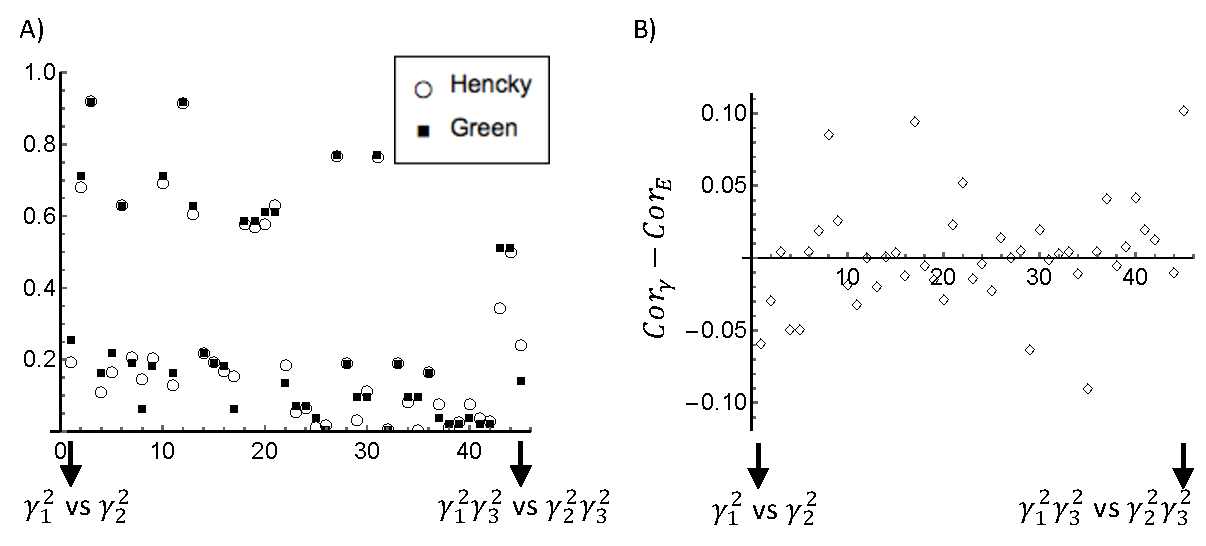
\includegraphics[width=6.0in]{Figures/gvsecorrelationeff}
\caption{(A) The correlation between parameters pairs in $\Psi_{eff}$ (Eqn. \ref{eqn:finalexponentialmodelformscaled}) when using Green-Lagrange vs Hencky strains. (B) The difference in correlation between each pair of parameters is minimal.}
\label{fig:gvsecorrelationeff}
\end{figure}
%-------------------	 end FIGURE 	-------------------%
%%%%%%%%%%%%%%%%%%%%%%%%%%%%%%%%%%%%%%%%%%%%%%%%%%%%%%%%%%%%


%%%%%%%%%%%%%%%%%%%%%%%%%%%%%%%%%%%%%%%%%%%%%%%%%%%%%%%%%%%%
%-------------------	begin FIGURE 	-------------------%
\begin{figure}
\centering
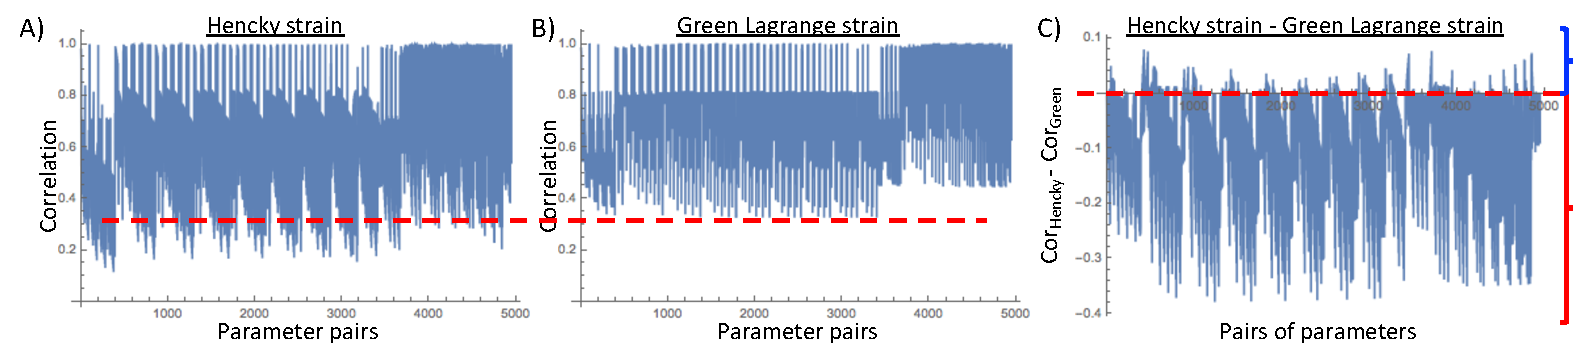
\includegraphics[width=6.5in]{Figures/gvsecorrelationpoly}
\caption{(A) The correlation between parameters pairs in a polynomial series type model with powers up to 6 when using Green-Lagrange vs (B) Hencky strains. (C) The difference in correlation between each pair of parameters. The red bracketed terms are benefited from using Hencky strains whereas the significantly fewer blue bracketed terms has better correlations with Green-Lagrange strain.}
\label{fig:gvsecorrelationpoly}
\end{figure}
%-------------------	 end FIGURE 	-------------------%
%%%%%%%%%%%%%%%%%%%%%%%%%%%%%%%%%%%%%%%%%%%%%%%%%%%%%%%%%%%%
















%---------------	specific form for BP	---------------%
\setcounter{figure}{0}
\setcounter{table}{0}
\setcounter{equation}{0}
\section{Specific effective constitutive model form for heart valve tissues replacements} \label{sec:specificform}

%%%%%%%%%%%%%%%%%%%%%%%%%%%%%%%%%%%%%%%%%%%%%%%%%%%%%%%%%%%%
%-------------------	begin FIGURE 	-------------------%
\begin{figure}
\centering
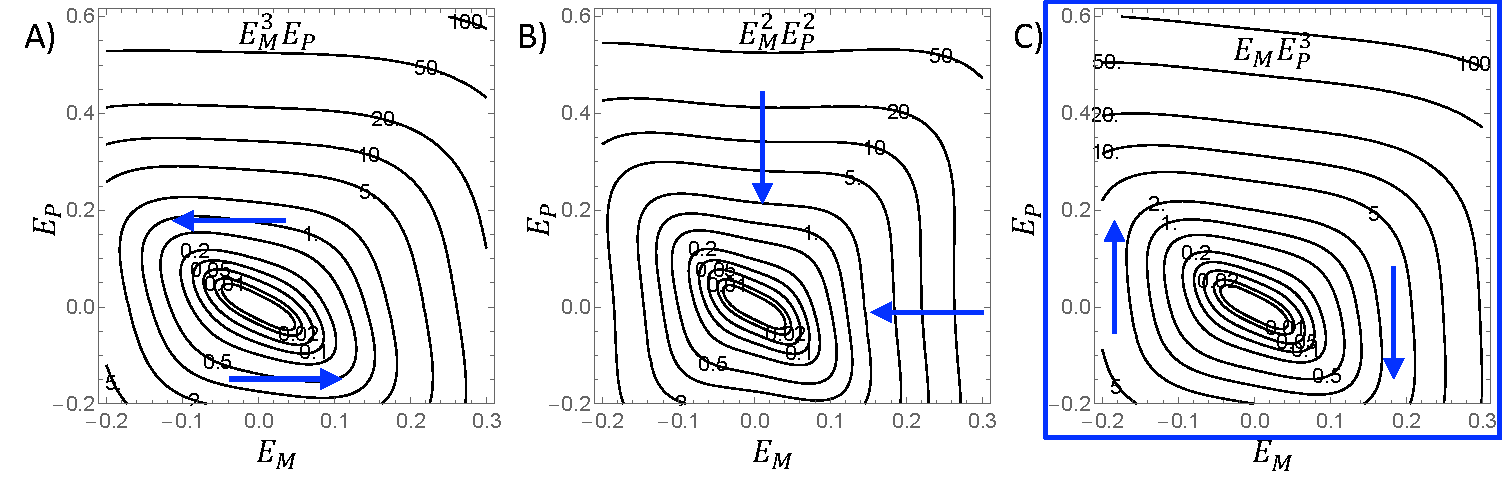
\includegraphics[width=6.5in]{Figures/couplingeffects}
\caption{The effect of the quartic coupling terms on the strain energy of $\Psi_{eff}$ (Eqn. \ref{eqn:finalexponentialmodelformscaled}). A) $E_m^3E_n$, shear of the $n$-axis. B)$E_m^2E_n^2$, squeezing. C)$E_mE_n^3$, shear of the $m$-axis.}
\label{fig:couplingeffects}
\end{figure}
%-------------------	 end FIGURE 	-------------------%
%%%%%%%%%%%%%%%%%%%%%%%%%%%%%%%%%%%%%%%%%%%%%%%%%%%%%%%%%%%%

    
	In some cases, it is possible to further reduce the form of $\Psi_{eff}$ (Eqn. \ref{eqn:finalexponentialmodelformscaled}). This may be helpful for reducing the cost of parameter estimation and parameter covariance. This depends on the coupling in the mechanical response of the material. For example, the $E_m$-$E_n$ coupling in most collagenous soft tissues (Fig. \ref{fig:couplingeffects}A) best match the behavior of the $E_m E_n^3$ term. This is because more fibers in the soft tissues are aligned to the material axis by definition, thus the effect of fiber rotation and thus coupling along this axis is generally less significant. Since $E_m^3 E_n$, $E_m^2 E_n^2$, and $E_m E_n^3$ are highly covariant terms in $\Psi{eff}$ (Eqn. \ref{eqn:finalexponentialmodelformscaled}). Each term affects the response of $\Psi_{eff}$ differently. Namely $E_m^2 E_n^2$ increases or decreases the roundedness of the contours (Fig. \ref{fig:couplingeffects}B), $E_m^3 E_n$ causes a shear of the S-axis (Fig. \ref{fig:couplingeffects}A), and $E_m E_n^3$ causes the shear of the M-axis (Fig. \ref{fig:couplingeffects}C). However, there is a only modest difference between the quality of fit between any combination of these three terms, $\Delta R^2<0.01$. Of these $E_m E_n^3$ gives the lowest $R^2$ and thus only $E_m E_n^3$ is necessary for $\Psi_{eff}$. Likewise, $E_m E_n E_\phi^2$ may not be needed due to low coupling between $E_m$-$E_n$, as observed in Sun et al. \cite{sun_biaxial_2003}. In some cases, it may be beneficial to separate the response of the matrix from those of collagen fiber and other components of the tissue, so it can be updated independently by the micro-models. In this case, $E_\phi^2$ is not necessary as the matrix modulus, thus the shear modulus, is zero and the $E_\phi^4$ will be able to describe shear stresses due to collagen fibers. As such, an example of the reduce form of the effective constitutive model for heart valve tissue replacements is
%==========================================================%
%-------------------	begin EQUATION 	-------------------%
\begin{equation}
\begin{aligned}\label{eqn:finalmodelform}
\Psi	=& c_0 \left(e^{Q} - 1\right) + \frac{\eta_M}{2} \left( \frac{1}{a}\left( I_1 -3\right)^{a} + \frac{r}{b} \left( I_1 -3\right)^{b} \right) - p\left(\mathrm{J}-1\right)\\
Q		=& b_1 E_m^2 + b_2 E_n^2 + b_4 E_m E_n + b_5 E_m^4 + b_6 E_n^4 + b_9 E_m E_n^3	\\
	&+ b_{10} E_\phi^4 + b_{11} E_m^2E_\phi^2 + b_{12} E_n^2 E_\phi^2,
\end{aligned}
\end{equation}
%-------------------	 end EQUATION 	-------------------%
%==========================================================%
where $\alpha$, $\beta$, and $r$ are pre-specified constants, p is the Lagrange multiplier for incompressibility, $\mu_M$ is the matrix modulus, and $c_0, b_1,...b_{12}$ are the remaining model parameters.






\setcounter{figure}{0}
\setcounter{table}{0}
\setcounter{equation}{0}
\section{Biaxial mechanical testing simulation}\label{sec:biaxialsimulation}

	A square patch was used to represent the soft tissue. An equivalent of 1 MPa in first Piola-Kirchhoff stress was applied evenly at nodal points along the edge of the patch, with varying direction for the material axis. The deformation within the patch was computed, and the resulting mechanical response was compared to analytical solution of $\Psi_{eff}$ (Eqn. \ref{eqn:finalexponentialmodelformscaled}). No difference in the resulting response was found. 

\begin{figure}[!htbp]
\centering
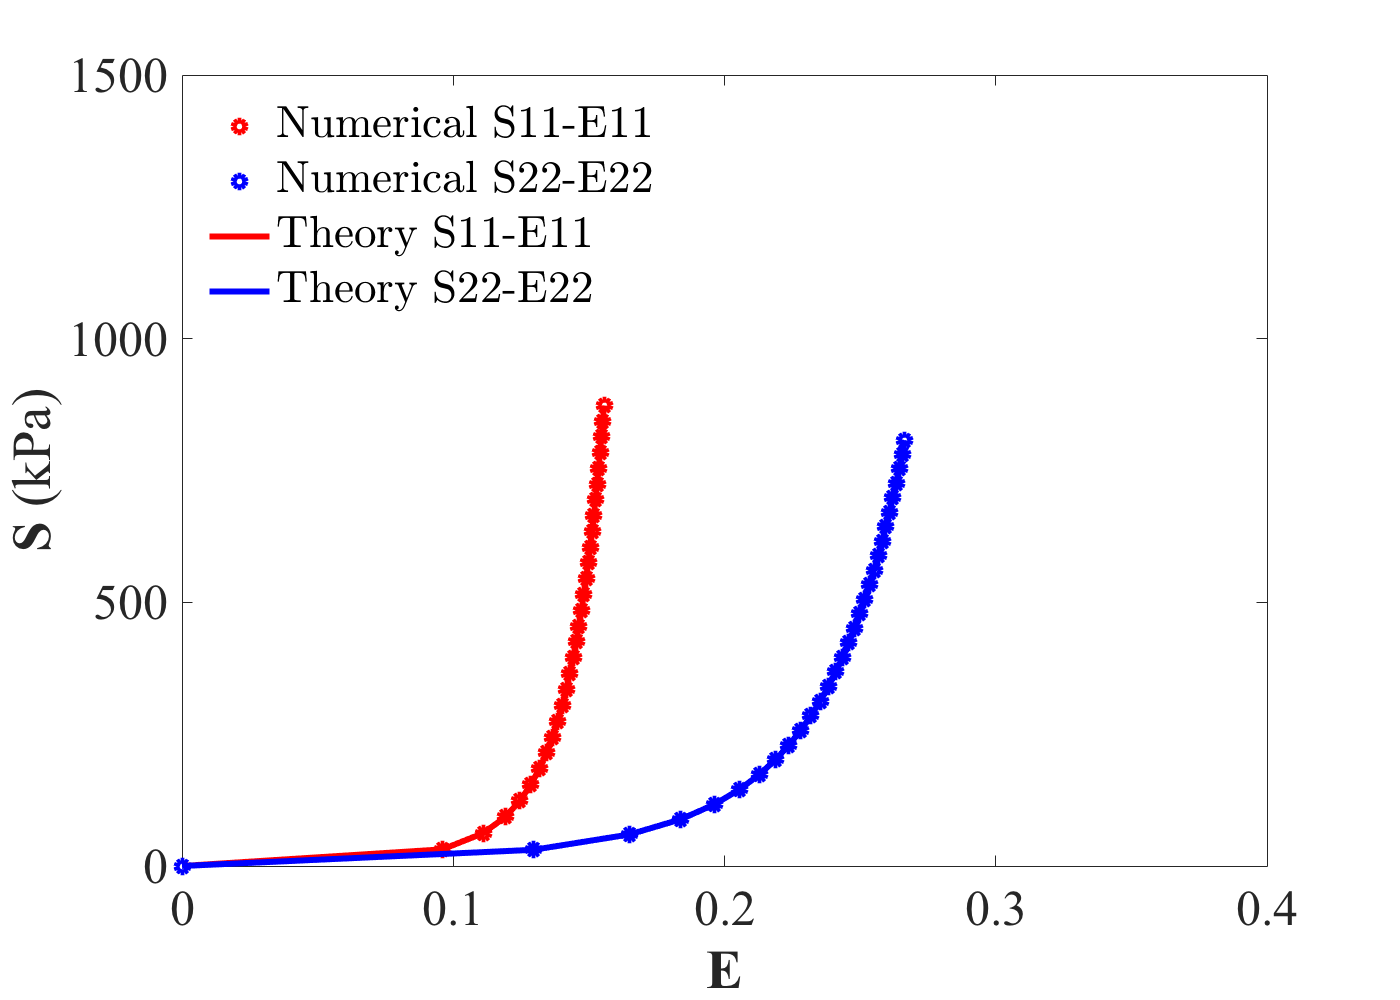
\includegraphics[width=3.25in]{Figures/validation.png}
\caption{Verification and validation of the correct implementation of the constitutive model where predicted Green’s strains from an equibiaxial loading path of a single IGA element compared with the theoretical result demonstrating exact agreement (left).}
\label{fig:biaxvalidation}
\end{figure}

\setcounter{figure}{0}
\setcounter{table}{0}
\setcounter{equation}{0}
\section{Optimal \textit{in silico} loading paths} \label{sec:optimalpaths}

	The most optimal loading path is the equibiaxial stress loading paths. This is not surprising as the equibiaxial stress response generally given very intuitive information on the mechanical response of soft tissues. Any odd number of loading paths will include the equibiaxial stress loading paths (Fig. \ref{fig:oddpaths}). Even when the number is even, we can observe that at least a few protocols are nearly equibiaxial in stress (Fig. \ref{fig:evenpaths}). For this reason, using an odd number of loading paths is highly recommended, as they will always include the minimal necessary set of loading paths, with the rest being average ratios in between (Fig. \ref{fig:oddpaths}). Even number of loading paths are generally very in consistent, and change slightly with each additional pairs of loading paths.  

%%%%%%%%%%%%%%%%%%%%%%%%%%%%%%%%%%%%%%%%%%%%%%%%%%%%%%%%%%%%
%-------------------	begin FIGURE 	-------------------%   
\begin{figure}
\centering
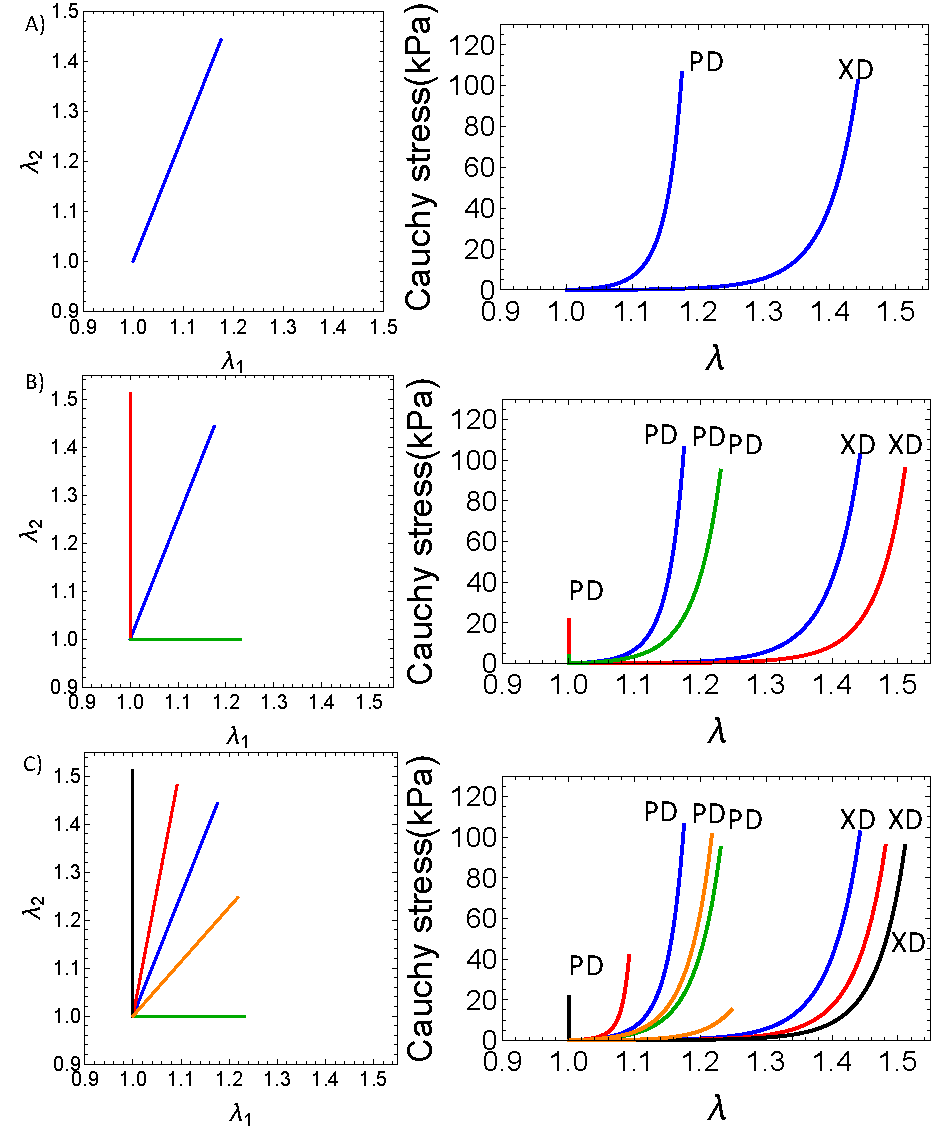
\includegraphics[width=6.5in]{Figures/oddpaths}
\caption{The optimal loading paths for generating data for a given total odd number of paths as well as the associated mechanical response, which is consistently containing the equi-biaxial stress loading path and the loading paths at the boundary.}
\label{fig:oddpaths}
\end{figure} 
%-------------------	 end FIGURE 	-------------------%
%%%%%%%%%%%%%%%%%%%%%%%%%%%%%%%%%%%%%%%%%%%%%%%%%%%%%%%%%%%%


%%%%%%%%%%%%%%%%%%%%%%%%%%%%%%%%%%%%%%%%%%%%%%%%%%%%%%%%%%%%
%-------------------	begin FIGURE 	-------------------%   
\begin{figure}
\centering
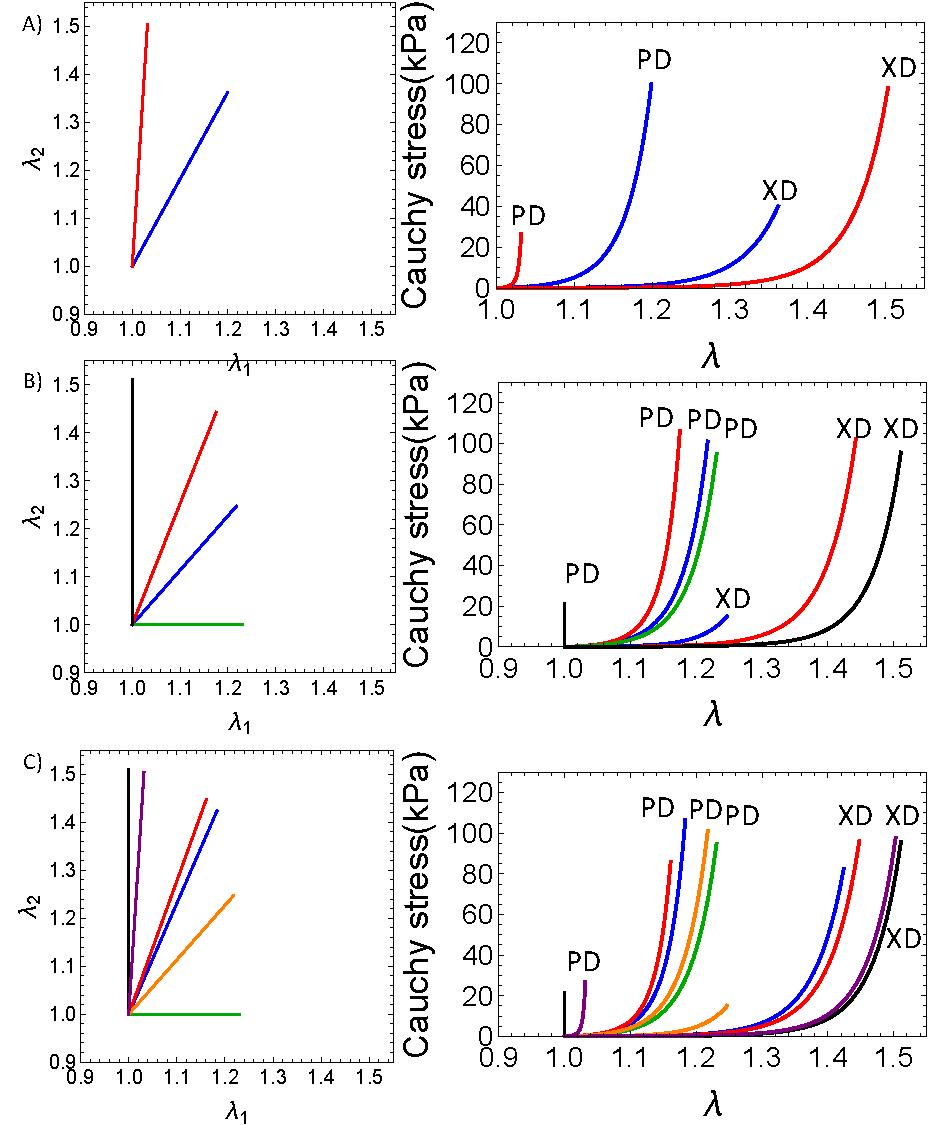
\includegraphics[width=6.5in]{Figures/evenpaths}
\caption{The optimal loading paths for generating data for a given even total number as well as the associated mechanical response, which is much more unpredictable than the odd (Fig. \ref{fig:oddpaths}) but gravitates towards the boundaries and the equi-biaxial loading paths as the number increases.}
\label{fig:evenpaths}
\end{figure} 
%-------------------	 end FIGURE 	-------------------%
%%%%%%%%%%%%%%%%%%%%%%%%%%%%%%%%%%%%%%%%%%%%%%%%%%%%%%%%%%%%

\setcounter{figure}{0}
\setcounter{table}{0}
\setcounter{equation}{0}
\section{Additional results for other tissue types and effective constitutive model forms} \label{sec:otherresults}

	Bovine pericardium is a good soft tissue to start with due high axes stretch coupling from their broad fiber splays. However, soft tissue behavior is drastically different with greater degree and anisotropy. For example aortic valve leaflets have larger elastin content resulting in larger toe region and extremely narrow ODFs, which can cause contraction along the material axis under equi-biaxial tension \cite{billiar_biaxial_2000b}. This behavior is hard for most constitutive models to replicate. However, $\Psi_{eff}$ (Eqn. \ref{eqn:finalexponentialmodelformscaled}) has no problem replicating this behavior (Fig. \ref{fig:aorticfit}). 

%%%%%%%%%%%%%%%%%%%%%%%%%%%%%%%%%%%%%%%%%%%%%%%%%%%%%%%%%%%%
%-------------------	begin FIGURE 	-------------------%
\begin{figure}
\centering
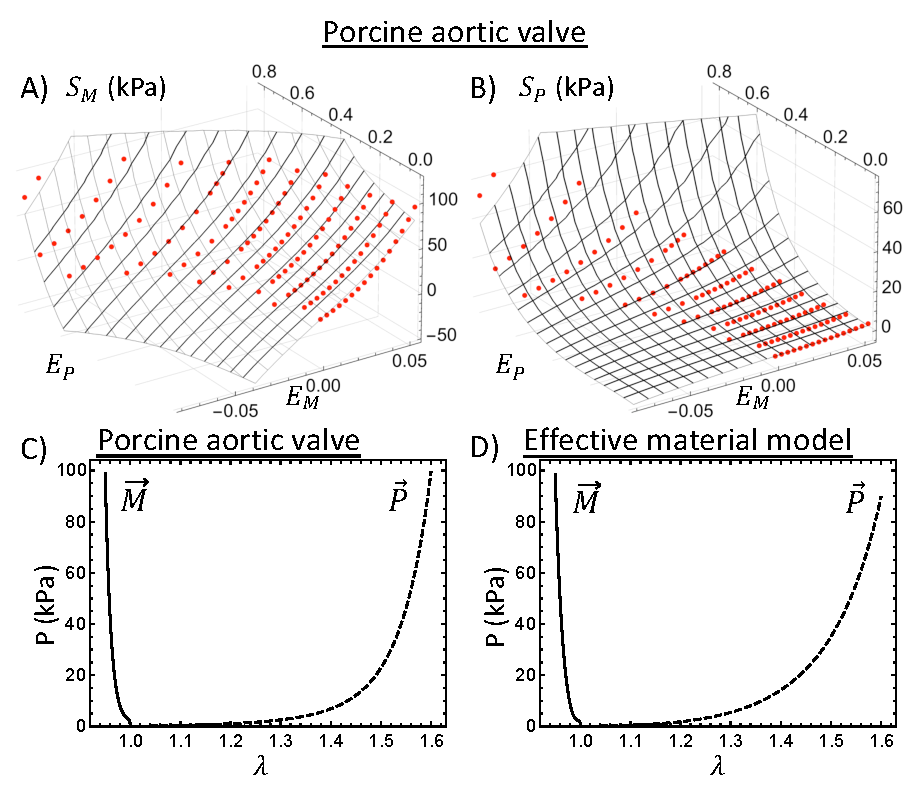
\includegraphics[width=6.5in]{Figures/aorticfit}
\caption{Parameter estimation results for porcine aortic valve specimen with highly align collagen fibers, $\sigma_{ODF} =10\deg$. The response function A) $S_m$ and b) $S_n$ are shown. C) This specimen contracts in the preferred fiber direction under equi-biaxial tension, a trait of soft tissues with highly aligned collagen fibers. D) $\Psi_{eff}$ (Eqn. \ref{eqn:finalexponentialmodelformscaled}) is able to reproduce this effect.}
\label{fig:aorticfit}
\end{figure} 
%-------------------	 end FIGURE 	-------------------%
%%%%%%%%%%%%%%%%%%%%%%%%%%%%%%%%%%%%%%%%%%%%%%%%%%%%%%%%%%%%
    
    Based on D-optimality, we determined the optimal loading paths and shown its importance for model predictability. The equi-biaxial stress loading path (near equi-biaxial) came out as especially important, as it is included in all sets of optimal loading paths except for two and four (Fig. \ref{fig:oddpaths}\&\ref{fig:evenpaths}). Commonly, when reproducing results from older publication, only the equi-biaxial stress loading path may be included in the figures as it is the most informative. Indeed, using the equi-biaxial stress loading paths simply results in much higher D-optimality than other choices. However, using this loading path alone is not sufficient for parameter estimation. Although the quality of fit is very good (Fig. \ref{fig:effequifit}A\&B), it cannot predict other loading paths (Fig. \ref{fig:effequifit}C\&D) 
    
%%%%%%%%%%%%%%%%%%%%%%%%%%%%%%%%%%%%%%%%%%%%%%%%%%%%%%%%%%%%
%-------------------	begin FIGURE 	-------------------%
\begin{figure}[!hbtp]
\centering
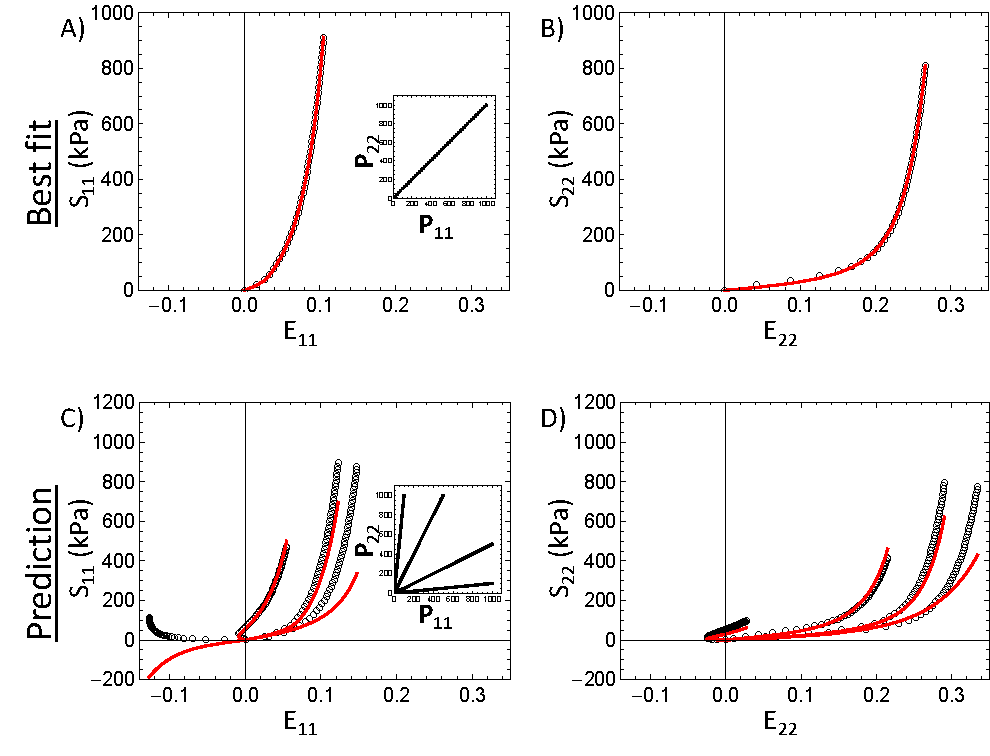
\includegraphics[width=6.5in]{Figures/effequifit}
\caption{$\Psi_{eff}$ fitting to a single equi-biaxial loading path, showing the A) $S_{11}$ and B) $S_{22}$ component. The prediction for the C) $S_{11}$ component and D) $S_{22}$ component of the unfitted loading paths are poor. The inset in C shows the corresponding loading paths.}
\label{fig:effequifit}
\end{figure} 
%-------------------	 end FIGURE 	-------------------%
%%%%%%%%%%%%%%%%%%%%%%%%%%%%%%%%%%%%%%%%%%%%%%%%%%%%%%%%%%%%

	With the addition of other loading paths, even non-optimal, this can significantly improve the predictive capabilities (Fig. \ref{fig:modelspred}A\&B). However, we can clearly see that because the loading paths are not optimal, the $0.1/1$ loading path is not predicted very well (Fig. \ref{fig:modelspred}B). We tested to see if this can be improved through more specific forms of $\Psi_{eff}$ (Eqn. \ref{eqn:finalexponentialmodelformscaled}). For this, we looked at an extension of the generalized Fung model to quadratic terms presented by Sun \textit{et al.} \cite{sun_biaxial_2003} to better fit the response of the glutaraldehyde cross-linked bovine pericardium. The additional terms are only of cubic and quartic powers, $B_{ijkl}E_{ij}^2E_{kl}^2$. In comparison to $\Psi_{eff}$, this is only missing $E_m^3E_n$ and $E_m^3E_n$,
%==========================================================%
%-------------------	begin EQUATION 	-------------------%
\begin{equation}\label{eqn:fullsunmodel}
\begin{aligned}
\Psi	=& c_0 \left(e^{Q} - 1\right) \\
Q		=& A_1 E_{11}^2 + A_2 E_{22}^2 + 2A_3E_{11}E_{22} + A_4 E_{12}^2 + 2A_5E_{12}E_{11}	\\
	&+ 2A_6E_{12}E_{22} + B_1 E_{11}^4 + B_2 E_{22}^4 + 2B_3E_{11}^2E_{22}^2 + B_4 E_{12}^4	\\
    &+ 2B_5E_{12}^2E_{11}^2 + 2B_6E_{12}^2E_{22}^2 
\end{aligned}\tag{Sun et al. \cite{sun_biaxial_2003} Eqn. 4}
\end{equation}
%-------------------	 end EQUATION 	-------------------%
%==========================================================%   
We will call this the extended Fung model. In addition, Sun \textit{et al.} \cite{sun_biaxial_2003} also recommended a more minimalistic form, where only the coupling term $2B_3E_{11}^2E_{22}^2$ is added as , 
%==========================================================%
%-------------------	begin EQUATION 	-------------------%
\begin{equation}\label{eqn:extendedfung}
\begin{aligned}
\Psi	=& c_0 \left(e^{Q} - 1\right) \\
Q		=& A_1 E_{11}^2 + A_2 E_{22}^2 + 2A_3E_{11}E_{22} + A_4 E_{12}^2 + 2A_5E_{12}E_{11}	\\
	&+ 2A_6E_{12}E_{22} + 2B_3E_{11}^2E_{22}^2 + B_4 E_{12}^4.
\end{aligned}
\end{equation}
%-------------------	 end EQUATION 	-------------------%
%==========================================================% 
We shall call this the Sun model. 

	Although the equality of fit are all equally as good \ref{fig:modelsfit}, the extended Fung model (Eqn. \ref{eqn:fullsunmodel}) predicts $S_{22}$ component of the 0.1/1 loading path much better, but predicts the wrong sign for $S_{11}$ for the same loading path, as well as predicting the 1/0.1 loading path worse (Fig. \ref{fig:modelspred}C\&D). The Sun model (Eqn. \ref{eqn:extendedfung}) on the other hand is similar to $\Psi_{eff}$ but worse at predicting $S_{11}$ of the 1/0.1 loading path (Fig. \ref{fig:modelspred}E\&F). It's hard to predict how these constitutive models will behave when the loading paths are not optimal. This is especially true when only a single protocol is used, where predictions for all other protocols can be very poor (Fig. \ref{fig:effequifit}). However, as little as three loading paths are needed to fully reproduce the mechanical response of soft tissue over the entire range of deformations (Fig. \ref{fig:effoptpred}).
%%%%%%%%%%%%%%%%%%%%%%%%%%%%%%%%%%%%%%%%%%%%%%%%%%%%%%%%%%%%
%-------------------	begin FIGURE 	-------------------%
\begin{figure}[!hbtp]
\centering
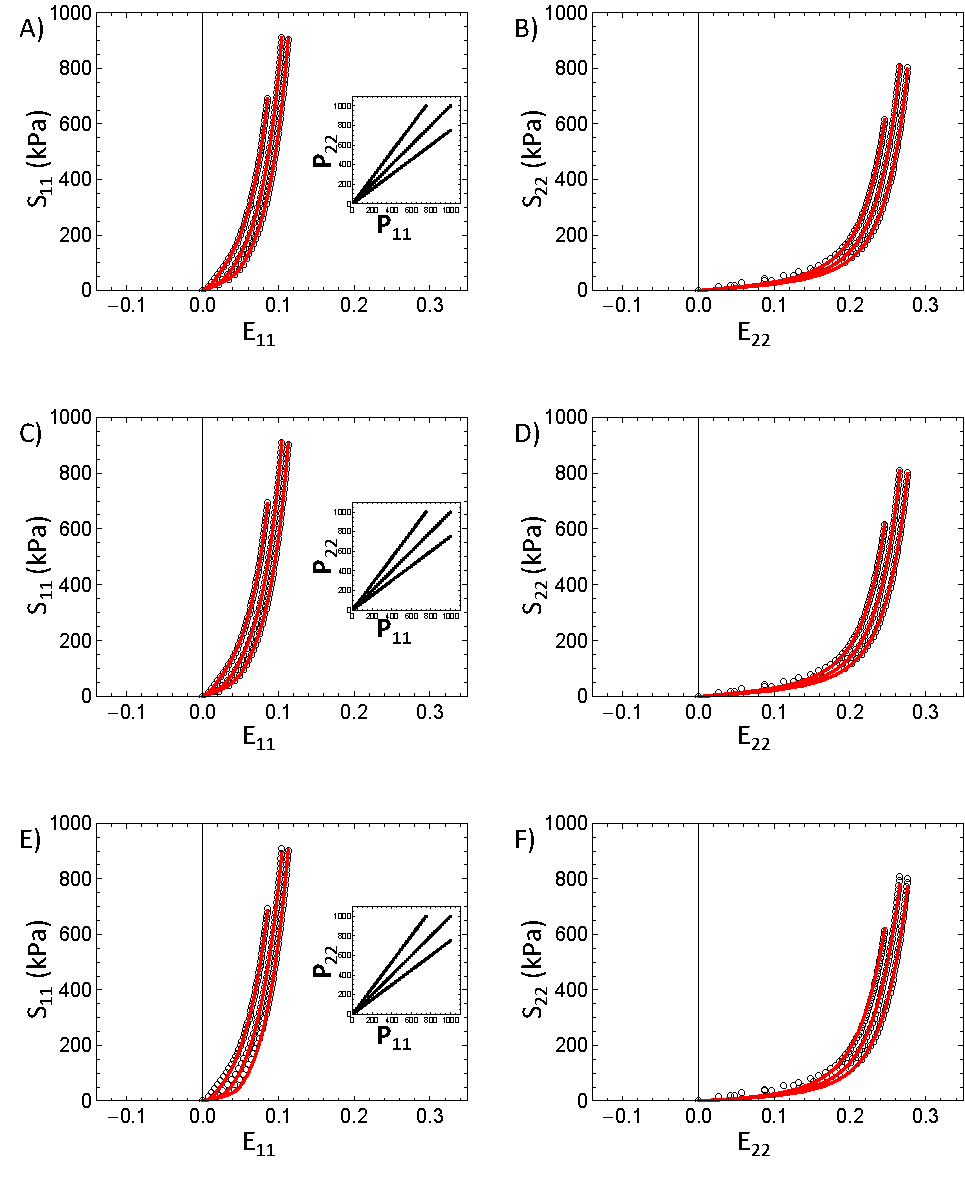
\includegraphics[width=6.5in]{Figures/modelsfit}
\caption{All three models, A\&B) $\Psi_{eff}$ (Eqn. \ref{eqn:finalexponentialmodelformscaled}), C\&D) extended Fung (\ref{eqn:fullsunmodel}), and E\&F) the Sun model (\ref{eqn:extendedfung}), can fit the data equally as well.}
\label{fig:modelsfit}
\end{figure} 
%-------------------	 end FIGURE 	-------------------%
%%%%%%%%%%%%%%%%%%%%%%%%%%%%%%%%%%%%%%%%%%%%%%%%%%%%%%%%%%%%

%%%%%%%%%%%%%%%%%%%%%%%%%%%%%%%%%%%%%%%%%%%%%%%%%%%%%%%%%%%%
%-------------------	begin FIGURE 	-------------------%
\begin{figure}[!hbtp]
\centering
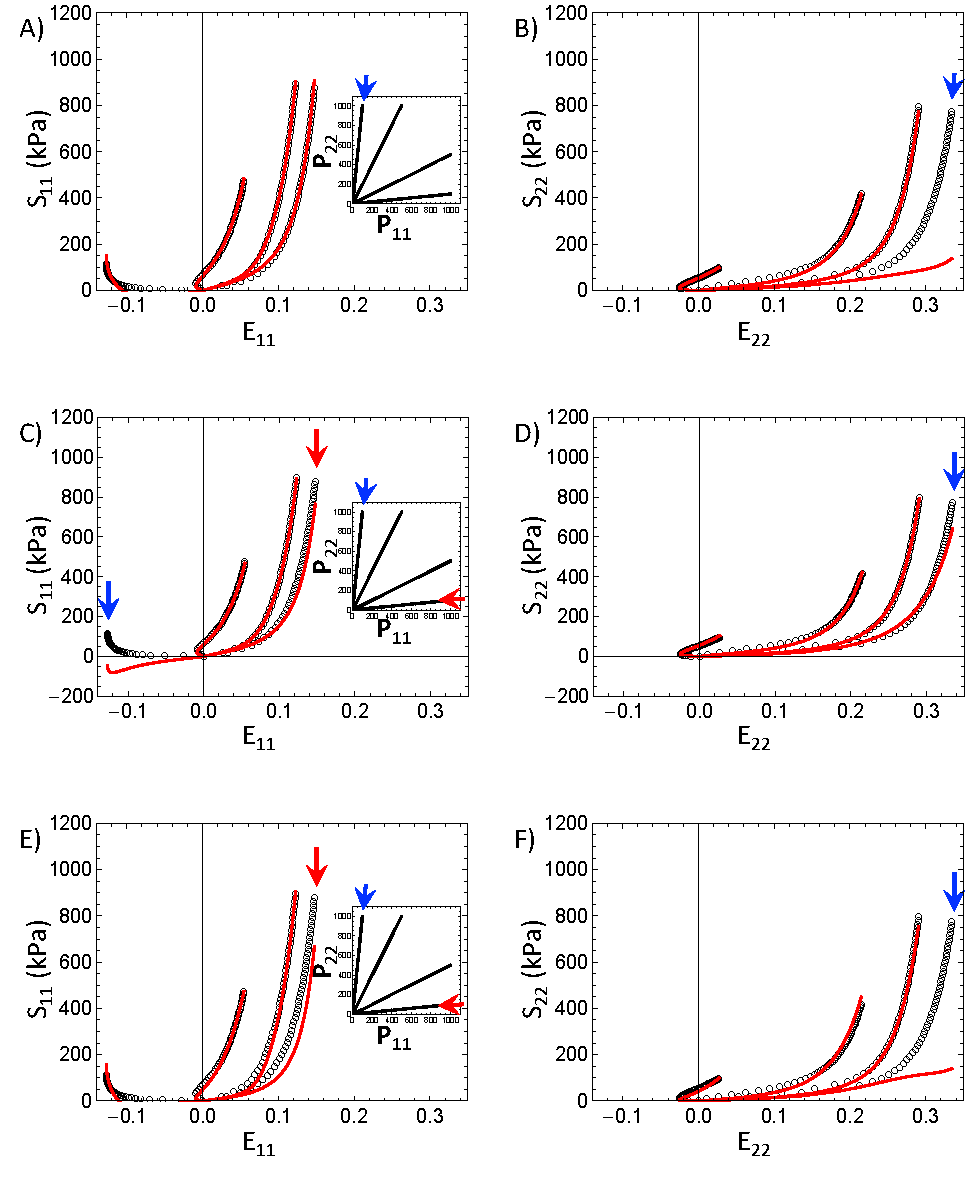
\includegraphics[width=6.5in]{Figures/modelspred}
\caption{Although the quality of fit are all equally as good \ref{fig:modelsfit}), the predictions for the unfitted loading paths are poor because the loading paths that were fit were not optimal. $\Psi_{eff}$ (Eqn. \ref{eqn:finalexponentialmodelformscaled}) predicts A) the $S_{11}$ component well, but B) the $S_{22}$ component of the $0.1/1$ loading path very poorly. The extended Fung (\ref{eqn:fullsunmodel}) predicts C) the $S_{11}$ component of both the $0.1/1$ and $1/0.1$ loading paths poorly, and D) the $S_{22}$ component of the $0.1/1$ loading path poorly. The Sun model (\ref{eqn:extendedfung}) is a slight improvement, only predicting E) the $S_{11}$ component of the $1/0.1$ loading path and F) the $S_{22}$ component of the $0.1/1$ loading path poorly. }
\label{fig:modelspred}
\end{figure} 
%-------------------	 end FIGURE 	-------------------%
%%%%%%%%%%%%%%%%%%%%%%%%%%%%%%%%%%%%%%%%%%%%%%%%%%%%%%%%%%%%




% %%%%%%%%%%%%%%%%%%%%%%%%%%%%%%%%%%%%%%%%%%%%%%%%%%%%%%%%%%%%
% %-------------------	begin FIGURE 	-------------------%
% \begin{figure}[hbtp]
% \centering
% \includegraphics[width=6.5in]{Figures/fungvseff}
% \caption{Comparing the effective constitutive model with the generalized Fung model at fitting the material response of soft tissues, showing the generalized Fung model when fitting to the A) physiological and B) non-physiological loading paths, as well as the effective constitutive model fitting to the C) five most optimal and D) three most optimal loading paths. Alternative types of loading paths were also tested. Including the use of p- and l-protocols in the post-pre-strain (p-p-E) range defined in Fung \textit{et al.} \cite{fung_pseudoelasticity_1979}. In this case, we shown the results for using D) one pair and F) three pairs of such protocols. Column 1-3 shows the quality of fit for each case, and column 4 shows the ability of the constitutive models to predict the remaining loading paths.}
% \label{fig:fungvseff}
% \end{figure} 
% %-------------------	 end FIGURE 	-------------------%
% %%%%%%%%%%%%%%%%%%%%%%%%%%%%%%%%%%%%%%%%%%%%%%%%%%%%%%%%%%%%


    
    

% %%%%%%%%%%%%%%%%%%%%%%%%%%%%%%%%%%%%%%%%%%%%%%%%%%%%%%%%%%%%
% %-------------------	begin FIGURE 	-------------------%   
% \begin{figure}
% \centering
% \includegraphics[width=6.5in]{Figures/nonoptimalpaths}
% \caption{Comparing parameter estimation results when fitting to non-optimal loading paths, using A) $\Psi_{eff}$ (Eqn. \ref{eqn:finalexponentialmodelformscaled}) and two other extensions to the generalized Fung models from Sun \textit{et al.} \cite{sun_biaxial_2003}, B) equation 4, which is an extension to the generalized Fung model by adding the quartic terms of $E_{11}^4$, $E_{22}^4$, $E_{12}^4$, $E_{11}^2 E_{22}^2$, $E_{11}^2 E_{12}^2$, and $E_{22}^2 E_{12}^2$ and C) equation 5 of said work, which is an extension to the generalized Fung model by adding the term $E_{11}^2 E_{22}^2$ only. D) $\Psi_{eff}$ was also fitted to only the equi-biaxial tension loading path and check for it's abilities to predict the remaining responses.}
% \label{fig:nonoptimalpaths}
% \end{figure} 
% %-------------------	 end FIGURE 	-------------------%
% %%%%%%%%%%%%%%%%%%%%%%%%%%%%%%%%%%%%%%%%%%%%%%%%%%%%%%%%%%%%













\end{appendices}




\end{document}








